\documentclass[spec, och, diploma]{SCWorks}
% параметр - тип обучения - одно из значений:
%    spec     - специальность
%    bachelor - бакалавриат (по умолчанию)
%    master   - магистратура
% параметр - форма обучения - одно из значений:
%    och   - очное (по умолчанию)
%    zaoch - заочное
% параметр - тип работы - одно из значений:
%    referat    - реферат
%    coursework - курсовая работа (по умолчанию)
%    diploma    - дипломная работа
%    pract      - отчет по практике
% параметр - включение шрифта
%    times    - включение шрифта Times New Roman (если установлен)
%               по умолчанию выключен
\usepackage{subfigure}
\usepackage{tikz,pgfplots}
\pgfplotsset{compat=1.5}
\usepackage{float}

%\usepackage{titlesec}
\setcounter{secnumdepth}{4}
%\titleformat{\paragraph}
%{\normalfont\normalsize}{\theparagraph}{1em}{}
%\titlespacing*{\paragraph}
%{35.5pt}{3.25ex plus 1ex minus .2ex}{1.5ex plus .2ex}

\titleformat{\paragraph}[block]
{\hspace{1.25cm}\normalfont}
{\theparagraph}{1ex}{}
\titlespacing{\paragraph}
{0cm}{2ex plus 1ex minus .2ex}{.4ex plus.2ex}

% --------------------------------------------------------------------------%


\usepackage[T2A]{fontenc}
\usepackage[utf8]{inputenc}
\usepackage{graphicx}
\graphicspath{ {./images/} }
\usepackage{tempora}

\usepackage[sort,compress]{cite}
\usepackage{amsmath}
\usepackage{amssymb}
\usepackage{amsthm}
\usepackage{fancyvrb}
% \usepackage{listings}
\usepackage{listingsutf8}
\usepackage{longtable}
\usepackage{array}
\usepackage[english,russian]{babel}

% \usepackage[colorlinks=true]{hyperref}
\usepackage{url}
\urlstyle{same} % Устанавливает стиль шрифта таким же, как в тексте
\usepackage{underscore}
\usepackage{setspace}
\usepackage{indentfirst} 
\usepackage{mathtools}
\usepackage{amsfonts}
\usepackage{enumitem}
\usepackage{tikz}
\usepackage{xcolor} % для цветных элементов

\definecolor{codegreen}{rgb}{0,0.5,0} % Цвет комментариев
\definecolor{codegray}{rgb}{0.5,0.5,0.5} % Цвет номеров строк
\definecolor{background}{rgb}{1,1,1} % Цвет фона

\lstdefinestyle{mystyle}{
    backgroundcolor=\color{background}, % Цвет фона
    commentstyle=\color{codegreen}\itshape, % Стиль комментариев
    keywordstyle=\color{blue}\bfseries, % Стиль ключевых слов
    numberstyle=\fontsize{11}{11}\selectfont\color{codegray},
    stringstyle=\color{red}, % Стиль строк
    basicstyle=\ttfamily\fontsize{11}{12}\selectfont, % Courier New, 11 пт, одинарный интервал
    breakatwhitespace=false,         
    breaklines=true,                 
    captionpos=b,                    
    keepspaces=true,                 
    numbers=left,                    
    numbersep=10pt,                  
    showspaces=false,                
    showstringspaces=false,
    showtabs=false,                  
    tabsize=4, % Настройка ширины табуляции
    extendedchars=true, % Поддержка расширенных символов
    % inputencoding=utf8, % Кодировка входных данных
    literate={а}{{\char224}}1 {б}{{\char225}}1 {в}{{\char226}}1 {г}{{\char227}}1 {д}{{\char228}}1 
         {е}{{\char229}}1 {ё}{{\char184}}1 {ж}{{\char230}}1 {з}{{\char231}}1 {и}{{\char232}}1 
         {й}{{\char233}}1 {к}{{\char234}}1 {л}{{\char235}}1 {м}{{\char236}}1 {н}{{\char237}}1 
         {о}{{\char238}}1 {п}{{\char239}}1 {р}{{\char240}}1 {с}{{\char241}}1 {т}{{\char242}}1 
         {у}{{\char243}}1 {ф}{{\char244}}1 {х}{{\char245}}1 {ц}{{\char246}}1 {ч}{{\char247}}1 
         {ш}{{\char248}}1 {щ}{{\char249}}1 {ъ}{{\char250}}1 {ы}{{\char251}}1 {ь}{{\char252}}1 
         {э}{{\char253}}1 {ю}{{\char254}}1 {я}{{\char255}}1
         {А}{{\char192}}1 {Б}{{\char193}}1 {В}{{\char194}}1 {Г}{{\char195}}1 {Д}{{\char196}}1 
         {Е}{{\char197}}1 {Ё}{{\char168}}1 {Ж}{{\char198}}1 {З}{{\char199}}1 {И}{{\char200}}1 
         {Й}{{\char201}}1 {К}{{\char202}}1 {Л}{{\char203}}1 {М}{{\char204}}1 {Н}{{\char205}}1 
         {О}{{\char206}}1 {П}{{\char207}}1 {Р}{{\char208}}1 {С}{{\char209}}1 {Т}{{\char210}}1 
         {У}{{\char211}}1 {Ф}{{\char212}}1 {Х}{{\char213}}1 {Ц}{{\char214}}1 {Ч}{{\char215}}1 
         {Ш}{{\char216}}1 {Щ}{{\char217}}1 {Ъ}{{\char218}}1 {Ы}{{\char219}}1 {Ь}{{\char220}}1 
         {Э}{{\char221}}1 {Ю}{{\char222}}1 {Я}{{\char223}}1,
}

\lstset{style=mystyle}


% \usepackage{minted}

\newcommand{\eqdef}{\stackrel {\rm def}{=}}
\newcommand{\specialcell}[2][c]{%
\begin{tabular}[#1]{@{}c@{}}#2\end{tabular}}

\renewcommand\theFancyVerbLine{\small\arabic{FancyVerbLine}}

\newtheorem{lem}{Лемма}

\begin{document}

% Кафедра (в родительном падеже)
\chair{теоретических основ компьютерной безопасности и криптографии}

% Тема работы
\title{Интеллектуальный анализ сетевого трафика: выявление RDP-сессий с помощью нейронных сетей}

% Курс
\course{6}

% Группа
\group{631}

% Факультет (в родительном падеже) (по умолчанию "факультета КНиИТ")
\department{факультета КНиИТ}

% Специальность/направление код - наименование
%\napravlenie{09.03.04 "--- Программная инженерия}
%\napravlenie{010500 "--- Математическое обеспечение и администрирование информационных систем}
%\napravlenie{230100 "--- Информатика и вычислительная техника}
%\napravlenie{231000 "--- Программная инженерия}
\napravlenie{10.05.01 "--- Компьютерная безопасность}

% Для студентки. Для работы студента следующая команда не нужна.
% \studenttitle{Студентки}

% Фамилия, имя, отчество в родительном падеже
\author{Токарева Никиты Сергеевича}

% Заведующий кафедрой
\chtitle{д. ф.-м. н., профессор} % степень, звание
\chname{Абросимов М. Б.}

%Научный руководитель (для реферата преподаватель проверяющий работу)
\satitle{доцент, к.ю.н.} %должность, степень, звание
\saname{Гортинский А. В.}

% Руководитель практики от организации (только для практики,
% для остальных типов работ не используется)
% \patitle{к.ф.-м.н.}
% \paname{С.~В.~Миронов}

% Семестр (только для практики, для остальных
% типов работ не используется)
%\term{8}

% Наименование практики (только для практики, для остальных
% типов работ не используется)
%\practtype{преддипломная}

% Продолжительность практики (количество недель) (только для практики,
% для остальных типов работ не используется)
%\duration{4}

% Даты начала и окончания практики (только для практики, для остальных
% типов работ не используется)
%\practStart{30.04.2019}
%\practFinish{27.05.2019}

% Год выполнения отчета
\date{2025}

\maketitle

% Включение нумерации рисунков, формул и таблиц по разделам
% (по умолчанию - нумерация сквозная)
% (допускается оба вида нумерации)
% \secNumbering

%-------------------------------------------------------------------------------------------

\tableofcontents

\intro

С увеличением объемов сетевого трафика и количества удаленных подключений задачи мониторинга и анализа сетевых данных становятся все 
более важными. Одним из основных протоколов для удаленного управления рабочими станциями и серверами является Remote Desktop Protocol 
(RDP). Он активно применяется в корпоративных и частных сетях, позволяя пользователям безопасно управлять удаленными системами. Вместе 
с тем популярность RDP делает его мишенью для атак злоумышленников, что подчеркивает важность задач его идентификации и мониторинга.

В наши дни существует множество различных подходов и методов анализа сетевого трафика. С развитием машинного обучения 
всё большую популярность набирают методы, использующие нейронные сети. В данной работе рассматривается модель рекуррентных 
нейронных сетей -- Long Short-Term Memory (LSTM), которая применяется для обнаружения RDP-сессий в сетевом трафике.

Целью работы является разработка программы для выявления RDP-трафика в сетевом потоке с использованием модели нейронной сети 
LSTM. Также работа направлена на демонстрацию того, что даже при зашифрованном трафике протоколы могут быть идентифицированы 
посредством анализа побочной информации, извлекаемой из пакетов. Для достижения этой цели 
были поставлены следующие задачи:

\begin{itemize}
    \item изучить особенности протокола RDP и его характерные признаки в сетевом трафике;
    \item разработать и вычислить метрики для анализа временных характеристик сетевого трафика;
    \item реализовать алгоритмы классификации на основе нейронной сети LSTM;
    \item создать программное обеспечение, способное в реальном времени анализировать трафик и идентифицировать RDP-сессии;
    \item провести тестирование системы и оценить её эффективность.
\end{itemize}

Данная работа связана с исследованиями в области анализа сетевого трафика и информационной безопасности, 
расширяя возможности автоматизированного мониторинга и предоставляя новые подходы для защиты систем от 
потенциальных угроз. Результаты исследования могут быть использованы для разработки инструментов защиты 
и контроля сетевого взаимодействия в корпоративных и частных сетях.


\section{Протокол RDP: место в сетях и особенности реализации}

Идея удалённого доступа к вычислительным ресурсам возникла из необходимости управления компьютерами и серверами, 
расположенными на расстоянии. Это дало пользователям возможность работать независимо от физического расположения 
оборудования, обеспечивая гибкость и эффективность использования вычислительной мощности.

Протокол удаленного рабочего стола (Remote Desktop Protocol, RDP) был разработан корпорацией Microsoft в конце 1990-х годов как решение для 
удаленного доступа к компьютерам и серверам. Истоки технологии удаленного доступа уходят в 90-е годы XX века, когда компании начали создавать 
протоколы для управления вычислительными системами на расстоянии. Одним из первых таких протоколов был Citrix ICA, который стал основой для 
создания RDP. Microsoft внедрила эту технологию в свои продукты, начиная с Windows NT Terminal Server 4.0, что значительно упростило удалённую работу.

\subsection{Обзор протокола RDP}

Создание RDP было мотивировано необходимостью предоставить пользователям возможность удаленно управлять вычислительными ресурсами вне зависимости 
от их физического размещения. Эта технология стала ключевым элементом корпоративных сетей, позволяя администраторам эффективно управлять серверами, 
а пользователям — работать с удаленными рабочими столами. Изначально RDP предназначался для работы в режиме точка-точка, но впоследствии он обрел 
поддержку многоточечных соединений, что превратило его в универсальный инструмент для коллективной работы и администрирования \cite{rdp22}.

RDP является расширением семейства протоколов T.120 и базируется на стандарте T.Share. Его ключевые особенности:

\begin{enumerate}
  \item Многоканальная архитектура: RDP поддерживает до 64 000 виртуальных каналов для передачи различных типов данных, таких как:
  
  \begin{itemize}
    \item данные презентации;
    \item управление периферийными устройствами;
    \item лицензирование;
    \item зашифрованные команды клавиатуры и мыши.
    
  \end{itemize}
  
  \item Безопасность: протокол включает механизмы шифрования, обеспечивающие защиту передаваемых данных. Это делает RDP надёжным выбором для корпоративных сетей;
  
  \item Универсальность: RDP изначально был разработан для работы с различными сетевыми топологиями, включая ISDN, POTS и TCP/IP. Современные версии фокусируются на TCP/IP, обеспечивая широкую совместимость;
  
  \item Оптимизация сетевого трафика: протокол использует компрессию данных и механизмы кадрирования для минимизации сетевых задержек;
  
  \item Поддержка мультимедиа: современные версии RDP включают функции передачи аудио, видео и взаимодействия с периферийными устройствами, такими как принтеры и USB-устройства.
\end{enumerate}


\subsection{Место RDP в стеке протоколов}

Стек протоколов представляет собой набор взаимосвязанных стандартов и правил, определяющих взаимодействие между различными уровнями сетевой 
архитектуры. Каждый уровень отвечает за выполнение определённых функций, начиная от передачи данных через физические среды до обеспечения 
высокого уровня абстракции для приложений. Существует несколько моделей сетевых взаимодействий, каждая из которых предлагает свой подход 
к организации передачи данных между устройствами в сети.

Наиболее известным примером стека протоколов является модель OSI (Open Systems Interconnection), которая состоит из семи уровней:

\begin{enumerate}
  \item Физический уровень, который отвечает за передачу последовательности битов через канал связи.
  \item Канальный уровень, где осуществляется разбиение данных на <<кадры>>, размер которых обычно достигает
  от несколько сотен до нескольких тысяч байтов.
  \item Сетевой уровень, на котором осуществляется структуризация и маршрутизация пакетов от отправителя к получателю.
  \item Транспортный уровень, функцией которого является передача надежных последовательностей данных произвольной
  длины через коммуникационную сеть от отправителя к получателю.
  \item Сеансовый уровень, на котором происходит поддержка сессии связи, уп-\\*равление взаимодействием между приложениями.  
  \item Уровень представления, который представляет данные в понятном для какой-либо конкретной машины виде.
  \item Прикладной уровень, предоставляющий набор интерфейсов для взаимодействия пользовательских процессов с сетью \cite{osi-model}.
\end{enumerate}

Вследствие этого, RDP является непосредственно протоколом прикладного уровня модели OSI, наряду с HTTP, FTP, SSH и многими другими. Стоит отметить, что 
в основном OSI применяется преимущественно в образовательных и теоретических целях. На практике используется модель TCP/IP, которая отражает
реальную организацию современных компьютерных сетей \cite{stack}. Она была разработана как часть стека протоколов, лежащих в основе интернета. 
Название TCP/IP связано с двумя ключевыми протоколами этого семейства -- Transmission Control Protocol (TCP) и Internet Protocol (IP). Именно они 
были впервые разработаны и задокументированы в этом стандарте. Иногда эту модель называют моделью DOD (Department of Defense) \cite{tcpip}.
TCP/IP используется повсеместно, поскольку большинство современных протоколов (HTTP, FTP, RDP) работают в рамках этой модели. Модель TCP/IP 
разделяет сетевое взаимодействие на четыре уровня, каждый из которых выполняет определённые функции:

\begin{enumerate}
    \item Сетевой интерфейс/канальный уровень (объединяет уровни 1 и 2 OSI): отвечает за физическую передачу данных.
    \item Сетевой уровень (аналог уровня 3 OSI): используется для маршрутизации данных (например, протокол IP).
    \item Транспортный уровень (аналог уровня 4 OSI): обеспечивает надежность передачи данных с помощью протоколов TCP и UDP.
    \item Прикладной уровень (соответствует уровням 5, 6 и 7 OSI): поддерживает приложения и службы, такие как HTTP, FTP, RDP и т.д.
\end{enumerate}

Основное преимущество TCP/IP в том, что это практическая модель, на основе которой построен интернет. Все современные сети работают 
с протоколами TCP/IP, поэтому в реальных системах она имеет приоритет.

Здесь важно понимать, что в компьютерных сетях все данные инкапсулируются и декапсулируются на различных уровнях модели TCP/IP.
Процесс инкапсуляции происходит так, что на каждом уровне стека 
протоколы добавляют свои заголовки: от уровня приложений до канального уровня. На этапе приема данные декапсулируются в обратном порядке, начиная 
с канального уровня и заканчивая уровнем приложений. 

Исходя из описания уровней, RDP в модели TCP/IP также относится к прикладному уровню. Поэтому, данные RDP сначала инкапсулируются в сегменты TCP, 
которые затем оборачиваются в IP-пакеты и кадры Ethernet для передачи по сети. На принимающем устройстве данные декапсулируются в обратном 
порядке, начиная с канального уровня и заканчивая уровнем приложений, уровнем RDP.

Для понимания процесса передачи данных от отправителя к получателю важно рассмотреть структуру пакетов, используемых в сетевых взаимодействиях. Далее
будет рассмотрена четырехуровневая структура модели TCP/IP от канального до прикладного. 


\subsubsection{Структура Ethernet-кадра}

На канальном уровне передача данных осуществляется с использованием Ethernet-кадра. Его структура представлена на рисунке \ref{eth-frame}.

\begin{figure}[H]
  \centering
  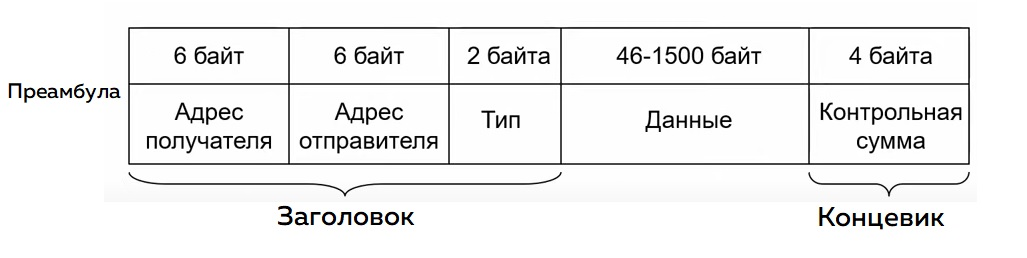
\includegraphics[width=0.9\textwidth]{pics/eth-frame.jpg}
  \caption{Структура Ethernet кадра}
  \label{eth-frame}
\end{figure}

Ключевыми полями Ethernet-кадра являются:

\begin{itemize}
  \item MAC-адреса источника и назначения -- позволяют определить отправителя и получателя на канальном уровне.
  \item Поле <<Тип>> -- указывает номер инкапсулированного сетевого протокола (например, IPv4 или IPv6).
  \item Поле данных -- содержит инкапсулированные данные более высокого уровня, включая сетевые пакеты.
\end{itemize}

\subsubsection{Структура IPv4-заголовка}

Для передачи TCP-сегментов на сетевом уровне используется IP-протокол. В данной работе рассматривается версия IPv4, 
так как её возможностей достаточно для анализа RDP-трафика. Структура IPv4-заголовка представлена на рисунке \ref{ipv4-header}.

\begin{figure}[H]
  \centering
  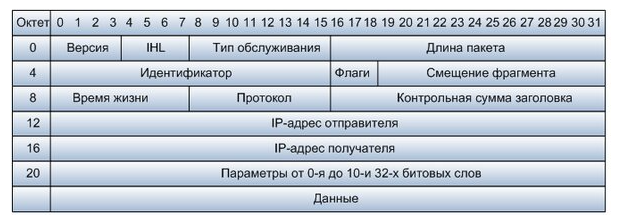
\includegraphics[width=0.9\textwidth]{pics/ipv4-header.png}
  \caption{Структура IPv4-заголовка}
  \label{ipv4-header}
\end{figure}

Особо важны следующие поля IPv4-заголовка:

\begin{itemize}
  \item IP-адреса отправителя и получателя -- позволяют идентифицировать ус-\\*тройства, участвующие в обмене данными.
  \item Поле <<Протокол>> -- определяет протокол транспортного уровня. Например, значение 6 указывает на TCP, а 17 -- на UDP.
\end{itemize}

\subsubsection{Структура заголовков TCP и UDP}

Известно, что протокол RDP взаимодействует с транспортным уровнем через TCP и UDP.
В основном данный протокол использует TCP для установления надёжного соединения и передачи данных, что позволяет обеспечить стабильное взаимодействие 
между клиентом и сервером удалённого рабочего стола. Сама структура TCP-заголовка показана на рисунке \ref{tcp-header}.

  \begin{figure}[H]
    \centering
    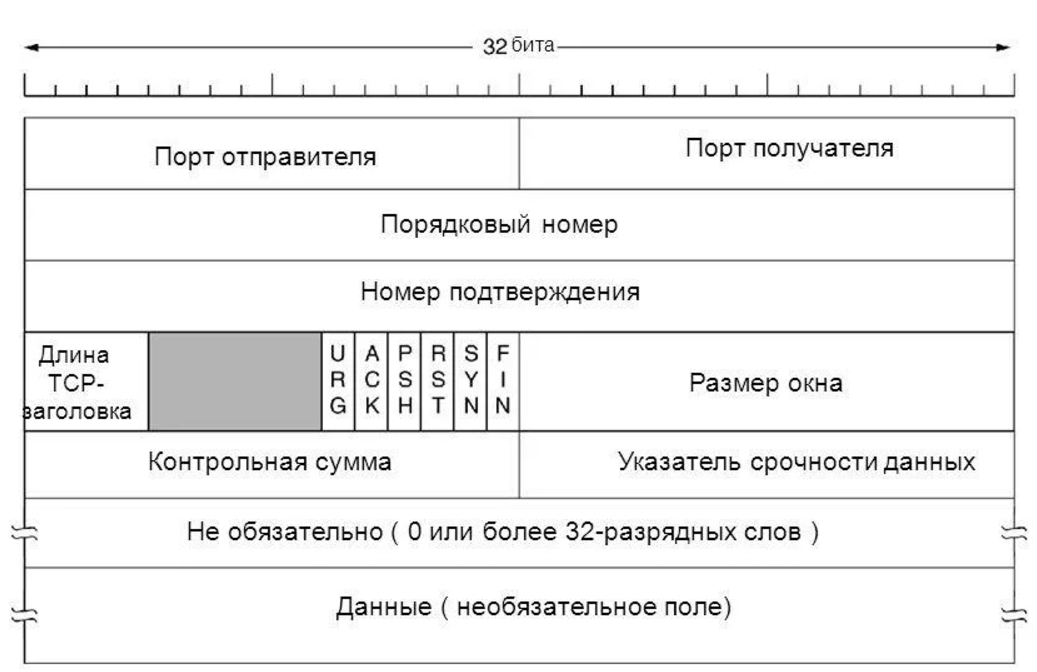
\includegraphics[width=0.9\textwidth]{pics/tcp-segment.png}
    \caption{Структура TCP-заголовка}
    \label{tcp-header}
  \end{figure}

В данном сегменте одними из интересных полей является информация о портах отправителя и получателя. Стоит отметить, что при подключении к 
удаленному рабочему столу по умолчанию используется порт 3389, что помогает идентифицировать RDP-трафик.

Не менее интересным полем является поле <<Размер окна>> -- это объем данных приема (в байтах), которые можно буферизировать во время подключения. 
Узел отправки может отправлять только этот объем данных, прежде чем он должен ожидать подтверждения и обновления окна от принимающего узла \cite{winsize}.
Другими словами, данная величина указывает количество байт, которое может быть отправлено без подтверждения от получателя до того момента, когда 
необходимо будет ожидать нового подтверждения о получении данных.

Также важное значение имеют флаги, содержащиеся в поле флагов. В нем хранятся следующие управляющие биты:

\begin{enumerate}
  \item NS -- одноразовая сумма (Nonce Sum). По-прежнему является экспериментальным флагом, используемым для защиты от случайного
  злонамеренного сокрытия пакетов от отправителя \cite{tcpflags}. Используется для улучшения работы механизма явного уведомления 
  о перегрузке (Explicit Congestion Notification, ECN).
  \item CWR -- окно перегрузки уменьшено (Congestion Window Reduced). 
  Данный флаг устанавливается (принимает значение равной единице) отправителем, чтобы показать, что TCP-фрагмент был
  получен с установленным полем ECE.
  \item ECE -- ECN-Эхо (ECN-Echo). Этот флаг показывает, поддерживает ли TCP-отправитель ECN.
  \item URG -- устанавливается, если необходимо передать ссылку на поле указателя срочности (Urgent pointer).
  \item ACK -- флаг подтверждения используется для подтверждения успешного получения пакета.
  \item PSH -- инструктирует получателя протолкнуть данные, накопившиеся в приемном буфере, в приложение пользователя.
  \item RST -- флаг сброса отправляется от получателя к отправителю, когда пакет отправляется на конкретный хост, который этого не ожидал.
  \item SYN -- начинает соединение и синхронизирует порядковые номера. Первый пакет, отправленный с каждой стороны, должен в обязательном порядке иметь установленным этот флаг.
  \item FIN -- означает, что данных от отправителя больше нет. Поэтому он используется в последнем пакете, отправленном отправителем.
\end{enumerate}

Они используются для управления соединением, передачи данных и завершения сессий.
Благодаря этим флагам можно определить текущее состояние соединения и характер обмена данными.

Поле <<Данные>> содержит информацию, которую передает приложение, использующее транспортный уровень. То есть, данные, которые 
находятся в этом поле, принадлежат уровню выше транспортного -- прикладному уровню. Таким образом, именно в этом поле хранятся данные о протоколе RDP.

Начиная с версии RDP 8.0 (введенной с Windows Server 2012 и Windows 8), протокол стал поддерживать UDP (англ. User Datagram Protocol -- протокол пользовательских датаграмм)
как дополнительный транспортный протокол для оптимизации работы в условиях нестабильных сетей \cite{udpseg}. Поэтому на структуру UDP протокола тоже стоит обратить внимание.
В отличие от TCP протокол UDP имеет минималистичный заголовок. Его можно увидеть на следующем рисунке.


\begin{figure}[H]
  \centering
  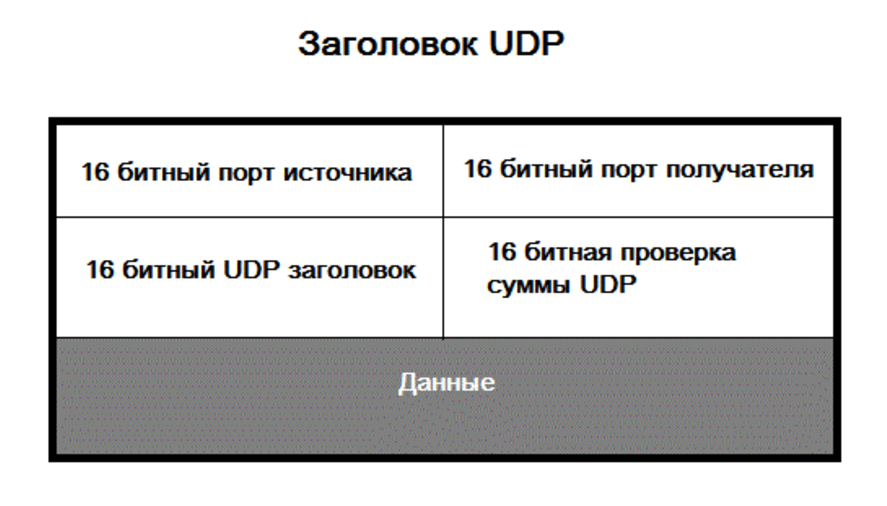
\includegraphics[width=0.9\textwidth]{pics/udp-segment.png}
  \caption{Структура UDP-заголовка}
  \label{udp-header}
\end{figure}

Из полезной информации можно выделить только номера портов и поле <<Данные>>.

Стоит отметить, что RDP использует UDP в случаях, когда нужно минимизировать задержки и повысить производительность, особенно для мультимедийных 
задач или нестабильных сетевых условий \cite{udpseg}. Однако TCP остаётся основным протоколом для критически важных операций, таких как 
управление соединением и передача данных с высокой надежностью.

Рассмотрение структуры пакетов, представленной в данном разделе, позволяет получить общее представление о принципах организации передачи данных в сетях и месте 
протокола RDP в стеке сетевых протоколов. Однако для решения задачи идентификации RDP-трафика среди общего потока данных возникают некоторые сложности.

Во-первых, RDP-трафик обычно передаётся в зашифрованном виде. Даже если программно получить доступе к полю данных в заголовках TCP и UDP, то расшифровка 
содержимого без наличия ключа шифрования становится практически невозможной \cite{lib5}. Это делает анализ RDP-заголовков недостаточно эффективным для точного 
определения наличия RDP-трафика.

Во-вторых, использование портов для идентификации RDP также не является надёжным методом. Злоумышленники могут изменить стандартный порт, 
применяемый для RDP-соединений, с целью избежать обнаружения. Более того, если на одном устройстве функционирует несколько RDP-сессий, для каждой 
из них могут использоваться разные порты, что дополнительно усложняет задачу анализа.

Таким образом, возникает вопрос: каким образом можно надёжно отличить трафик протокола удалённого рабочего стола от других протоколов, наблюдаемых в сетевой среде?

Ответ на данный вопрос будет рассмотрен в следующем разделе, где проанализированы ключевые метрики и особенности, характерные для RDP-трафика.

\section{Особенности и характерные признаки RDP-трафика}

В рамках моей предыдущей курсовой работы, посвящённой теме <<Статистический анализ сетевого трафика для обнаружения активной RDP-сессии>>, 
были изучены и применены различные методы статистического анализа для выявления RDP-трафика. В частности, рассматривались такие подходы, как:  

\begin{itemize}
  \item анализ распределения временных интервалов между пакетами;  
  \item исследование распределения размера пакетов;  
  \item анализ частоты флагов PSH;  
  \item нахождение отношения входящего и исходящего трафика.  
\end{itemize}

Результаты курсовой работы показали, что использование этих методов в совокупности позволяет с высокой степенью вероятности идентифицировать 
RDP-трафик в сетевой среде.  


В рамках настоящего исследования статистические методы рассматриваются более детально. Они дополняются новыми метриками, 
учитывающими динамические особенности RDP-сессий. Эти признаки используются в качестве входных данных для обучения нейронной сети, что позволяет 
значительно повысить точность и надёжность обнаружения RDP.

В данном разделе подробно описываются признаки, характерные для RDP-трафика и способы расчета метрик на основе этих признаков.
Все представленные метрики сопровождаются формулами и пояснениями их реализации в программной системе. Стоит отметить, что вся информация, 
используемая при вычислении метрик, собирается самой программой. Программа извлекает из перехваченных пакетов исключительно те данные, которые 
требуются для расчёта метрик.

\subsection{Признаки на основе анализа временных интервалов между сетевыми пакетами}

Анализ временных интервалов между пакетами может помочь выявить RDP-сессии. Как правило, промежутки между пакетами RDP-трафика короче, 
чем у других видов трафика. Это объясняется тем, что протокол RDP рассчитан на передачу данных в реальном времени и требует быстрой 
доставки информации для поддержания стабильного соединения с удаленным рабочим столом. Соответственно, если в сети наблюдается 
большое количество пакетов с короткими временными интервалами, это может свидетельствовать о наличии активной RDP-сессии. Тем 
не менее, важно помнить, что существуют и другие виды трафика, использующие высокие скорости передачи данных и характеризующиеся 
малыми интервалами между пакетами. Поэтому вычисляется несколько метрик, получаемые из промежутков временных интервалов, чтобы улучшить
процесс определения RDP-трафика.

\subsubsection{Вычисление задержки и стандартного отклонения временных интервалов между пакетами}

Под задержкой будем понимать среднее время, которое проходит между отправкой и получением пакетов. Пусть $ t_1, t_2, \dots, t_n $, 
где $ t_i $ -- это временная метка $ i $-го пакета. Разработанная программа запоминает все эти временные метки и находит разницу ($\Delta t_j$) 
между двумя пакетами следующим образом:
\begin{equation}
  \Delta t_j = t_{i+1} - t_{i}, \text{ для всех } i = \overline{1, n - 1}
\end{equation}

Тогда задержка вычисляется по следующей формуле:

\begin{equation}
  \mu_L = \frac{1}{n - 1} \sum_{i=1}^{n-1} \Delta t_i
\end{equation}

Исходя и формулы (2) можно заметить, что задержка -- это среднее значение временных интервалов между пакетами.

Вычисление стандартного отклонения, получается из значения задержки по следующей формуле:

\begin{equation}
  \sigma = \sqrt{\frac{1}{n-1} \sum_{i=1}^{n-1} (\Delta t_i - \mu_L)^2}
\end{equation}

  Среднее значение (задержка) и стандартное отклонение позволяет оценить стабильность интервалов времени 
  и, следовательно, стабильность передачи данных, что является одной из характерных черт RDP-трафика.

\subsubsection{Вычисление среднего джиттера и медианы временных интервалов}

   Джиттером называется изменение временной задержки между передачей данных и их получением по сетевому соединению.
   Проще говоря, джиттер отражает нестабильность задержки. Данная величина вычисляется по следующей формуле:

   \begin{equation}
      J_i = |\Delta t_{i+1} - \Delta t_i|, \quad \text{для } i = \overline{1, n - 2}.
   \end{equation}

  Тогда средний джиттер вычисляется следующим образом:

   \begin{equation}
    \mu_J = \frac{1}{n-2} \sum_{i=1}^{n-2} J_i
   \end{equation}

   Этот показатель характеризует, насколько стабильны интервалы между пакетов, что важно для оценки качества RDP-сессий, 
   поскольку низкий джиттер необходим для стабильной работы удаленного рабочего стола. 
   
   Исходя из формул вычисления задержки и джиттера может показаться, что эти величины похожи, но это не так. Они измеряют разные 
   аспекты передачи данных, и каждая из этих метрик имеет свое значение в контексте анализа RDP-трафика. Задержка показывает, как долго 
   передаются пакеты, а джиттер измеряет колебания этого времени.

   Медиана временных интервалов является также полезной метрикой, которая может помочь сгладить влияние выбросов и экстремальных значений. 
   Медиана представляет собой среднее значение в отсортированном ряду интервалов времени \cite{dev0}. Вследствие этого временные метки $t_i$ ($i = \overline{1, n}$) 
   перехваченных пакетов сортируются по возрастанию.
   
   Далее если количество интервалов $ n $ нечетное, то медианой будет центральный элемент отсортированного ряда. 
   Если $ n $ четное, медианой будет среднее значение двух центральных элементов.

   Таким образом медиана вычисляется следующим образом:

   \begin{equation}
    m_t = 
      \begin{cases}
        t_{n / 2}, & \text{если n нечетное}\\
        (t_{n / 2} + t_{n / 2 + 1}) / 2, & \text{если n четное}
      \end{cases}
   \end{equation}
  

\subsection{Признаки, связанные с количественными характеристиками трафика}


Помимо анализа временных интервалов, важную информацию о характере трафика можно получить из количественных характеристик передаваемых пакетов.
Анализ объёма и распределения трафика позволяет выявить ключевые закономерности, присущие протоколу RDP. Такие признаки, как соотношение 
входящего и исходящего трафика, распределение объёмов между UDP- и TCP-пакетами, а также средний размер передаваемых пакетов, отражают 
особенности поведения RDP-сессий. Каждый сетевой протокол обладает уникальным шаблоном обмена данными, и изучение этих характеристик 
играет важную роль в их идентификации.

\subsubsection{Вычисление отношения объема входящего на исходящий трафик}

Разработанная программа сохраняет пакеты относительно инициатора подключения (клиента) и целевого устройства (сервера). В процессе работы накапливаются 
две величины: объем исходящего трафика ($V_{src}$) — количество данных, отправляемых клиентом, и объем входящего трафика ($V_{dest}$) — количество данных, 
отправляемых сервером.

Отношение объема входящего на исходящий трафик вычисляется по формуле:

\begin{equation}
  r_{dest/src}^{init} = \frac{V_{dest}}{V_{src}}
\end{equation}

Аналогично отношение объема трафика относительно сервера вычисляется как:

\begin{equation}
  r_{dest/src}^{targ} = \frac{V_{src}}{V_{dest}}
\end{equation}

Эти две величины позволяют оценить симметричность обмена данными между клиентом и сервером. Для протокола RDP характерен асимметричный обмен 
трафиком: большая часть данных передается от сервера к клиенту, что обусловлено характером работы протокола, где сервер передает графическую 
информацию, а клиент отправляет команды управления.

Рассмотрение обеих величин важно, поскольку оно обеспечивает всесторонний анализ взаимодействия между клиентом и сервером. Например, высокое 
значение $r_{dest/src}^{init}$ (преобладание входящего трафика) может указывать на активность RDP-сессии, тогда как отклонения в этих показателях 
могут сигнализировать о другом типе соединения. Метрика особенно полезна в контексте других признаков, так как её устойчивость к шуму и вариативность 
в зависимости от типа трафика делает её важным элементом для классификации с использованием нейронной сети.

\subsubsection{Вычисление отношения объема UDP- и TCP-трафиков}

В предыдущем разделе упоминалось, что начиная с версии 8.0, протокол RDP поддерживает передачу данных по UDP. Это особенно заметно в 
сетевом обмене между компьютерами с установленной операционной системой Windows. По протоколу UDP в основном передаются графические данные, 
а также действия, совершаемые мышью и клавиатурой, что делает его важной частью работы RDP. Учитывая это, исключать анализ UDP-трафика из 
общей картины трафика было бы неправильно.

Разработанная программа отслеживает объем переданных пакетов по протоколам UDP и TCP, а также вычисляет их соотношение по следующей формуле:

\begin{equation}
  r_{udp/tcp} = \frac{V_{udp}}{V_{tcp}}
\end{equation}

Таким образом, данная метрика отражает баланс использования двух транспортных протоколов в рамках одного соединения \cite{lib1}. Для RDP характерно 
заметное преобладание трафика по протоколу TCP, однако наличие UDP-трафика с характерным объемом может служить дополнительным индикатором 
активности RDP-сессии.

Эта метрика становится особенно эффективной в сочетании с другими признаками, улучшая точность классификации сетевого трафика и выявления RDP.

\subsubsection{Вычисление среднего значения объема пакетов}

При работе протоколов прикладного уровня данные передаются пакетами различных объемов. 
Размер пакетов может меняться в зависимости от характера передаваемой информации: от небольших управляющих сообщений до крупных сегментов данных
Исследование размеров передаваемых пакетов может оказаться полезным инструментом при анализе сетевого 
трафика, особенно когда речь идет об определении аномалий или подозрительных активностей.


В разработанной программе анализируется размер блока «Данные», содержащегося в заголовках протоколов TCP и UDP. В процессе перехвата 
трафика программа сохраняет размеры полезной нагрузки каждого пакета: \\ $p_{s_1}, p_{s_2}, \dots, p_{s_n}$. На основании этих данных 
вычисляется среднее значение объема передаваемых пакетов:

\begin{equation}
  \mu_s = \frac{1}{n} \sum_{i=1}^{n} \Delta p_{s_i}
\end{equation}

Эта метрика предоставляет информацию о характере передаваемого трафика. Для протокола RDP характерен обмен пакетами малого и среднего 
размера, отражающий отправку управляющих сигналов, таких как движения мыши, нажатия клавиш, или обновления небольших частей экрана. В 
отличие от этого, потоки мультимедиа или файлы, передаваемые другими протоколами, обычно характеризуются значительно большими средними 
размерами пакетов.

Значимость среднего значения объема пакетов заключается в его способности идентифицировать типичные характеристики RDP-сессий и исключать 
несоответствующий трафик, тем самым улучшая точность анализа и классификации \cite{lib2, lib3}. В сочетании с другими метриками эта характеристика позволяет 
более точно выделять RDP-трафик среди общего потока сетевых данных.

\subsection{Признаки на основе анализа параметров TCP-соединений}

Протокол TCP предоставляет множество полей в своих заголовках, каждое из которых несет важную информацию о состоянии соединения, обмене данными и 
управлении потоком. Эти параметры играют ключевую роль в обеспечении надёжности передачи данных, но также могут служить источником ценной информации 
для анализа сетевого трафика.

В результате детального изучения особенностей сетевого взаимодействия по протоколу RDP были выявлены признаки, которые позволяют отличить данный 
тип трафика от других. Эти признаки связаны с использованием управляющих флагов TCP (PSH, ACK, SYN, FIN, RST), размером окна и другими параметрами, 
которые характеризуют поведение соединения.


\subsubsection{Вычисление частоты флагов PSH и ACK}

В контексте протокола RDP флаг PSH активно применяется для передачи пользовательских действий, таких как нажатия клавиш и движение мыши, 
а также для пересылки буферизованных изображений или звуковых данных. Наличие PSH-флагов может быть индикатором активности RDP-сессий, 
что делает их анализ полезным инструментом для идентификации такого трафика.

Для анализа частоты PSH-флагов разработанная программа подсчитывает количество TCP-пакетов с установленным флагом PSH для каждой стороны соединения. 
Это позволяет выделить:

\begin{itemize}
  \item $V_{P_{init}}$: объем входящего трафика с установленным флагом PSH относительно клиента;
  \item $V_{P_{targ}}$: объем входящего трафика с установленным флагом PSH относительно сервера;
  \item $V_{tcp}^{init}$: общее количество входящих TCP-пакетов, получаемых клиентом;
  \item $V_{tcp}^{targ}$: общее количество входящих TCP-пакетов, получаемых сервером.
\end{itemize}

На основе этих данных вычисляются частоты флагов PSH для каждой стороны.

Для клиента:

\begin{equation}
  r_{psh}^{init} = \frac{V_{P_{init}}}{V_{tcp}^{init}}
\end{equation}

Для сервера:

\begin{equation}
  r_{psh}^{targ} = \frac{V_{P_{targ}}}{V_{tcp}^{targ}}
\end{equation}

Анализ частоты PSH-флагов позволяет выявить характерный для RDP трафик, где их интенсивность выше, чем у большинства других протоколов. 
Рассмотрение этих метрик как относительно клиента, так и относительно сервера важно для учёта специфики взаимодействия между сторонами: 
данные клиента часто включают команды, а данные сервера — графическую или звуковую информацию. Такой двусторонний анализ помогает точнее 
охарактеризовать тип и особенности обмена данными.

Частота флагов ACK вычисляется аналогично частоте PSH-флагов. Программа накапливает данные о числе TCP-пакетов с установленным 
флагом ACK относительно клиента ($V_{A_{init}}$) и сервера ($V_{A_{targ}}$). После этого рассчитываются частоты ACK-флагов.

Для клиента:
  \begin{equation}
    r_{ack}^{init} = \frac{V_{A_{init}}}{V_{tcp}^{init}}
  \end{equation}

Для сервера:
  \begin{equation}
    r_{ack}^{targ} = \frac{V_{A_{targ}}}{V_{tcp}^{targ}}
  \end{equation}

  Анализ частоты ACK-флагов предоставляет информацию о количестве подтверждений, отправляемых и получаемых сторонами 
  соединения. В контексте RDP трафика частота ACK может отражать характер обмена данными, где сервер часто отправляет 
  подтверждения для поступающих от клиента команд и событий.

\subsubsection{Вычисление отношения ACK/PSH}

Для более детального анализа характерных признаков RDP-сессий программа также вычисляет отношения частот ACK- и PSH-флагов 
для клиента и сервера.

Для клиента:

\begin{equation}
  r_{ack/psh}^{init} = \frac{r_{ack}^{init}}{r_{psh}^{init}}
\end{equation}

Для сервера:

\begin{equation}
  r_{ack/psh}^{init} = \frac{r_{ack}^{targ}}{r_{psh}^{targ}}
\end{equation}

Данный подход объединяет две ключевые особенности RDP-трафика: интенсивное использование PSH-флагов для передачи данных сервером и 
частое подтверждение этих данных клиентом с помощью ACK-флагов.

RDP генерирует активный двусторонний трафик, где сервер отправляет значительные объемы данных (в том числе с PSH-флагами), 
а клиент, в свою очередь, регулярно отвечает подтверждениями (ACK-флагами). Вычисление отношения ACK/PSH позволяет выявить 
баланс между передачей данных и подтверждениями, что особенно важно для идентификации интерактивных сессий.

Эта комбинация признаков позволяет более точно отличать RDP-трафик от других видов трафика, где подобное поведение не столь выражено.

\subsubsection{Вычисление разности числа исходящих и входящих ACK-флагов}

Баланс между количеством подтверждений (ACK), отправленных и полученных в рамках TCP-сессии, может отражать динамику 
взаимодействия сторон. В интерактивных протоколах, таких как RDP, где клиент активно подтверждает получение данных от 
сервера, разность числа ACK-флагов может быть индикатором асимметрии трафика. Этот показатель предоставляет дополнительную 
информацию о характере передачи данных, что полезно для анализа таких сессий.

В программе вычисляется модуль разности числа TCP-пакетов с установленным флагом ACK, причем рассматривается только относительно клиента:

\begin{equation}
  d_{ack}^{init} = | V_{A_{src}} - V_{A_{dest}} |
\end{equation}

где $V_{A_{src}}$ -- число исходящих ACK-флагов от клиента, а $V_{A_{dest}}$ -- число входящих ACK-флагов, получаемых клиентом. В данном случае необязательно
еще вычислять разность исходящих и входящих ACK-флагов относительно сервера, так как данные величины будут одинаковы. Ведь вычисления проводятся под модулем.

Данная метрика полезна тем, что она позволяет выявить асимметрию в подтверждениях, характерную для RDP. Например, в типичной RDP-сессии 
клиент отправляет больше ACK-флагов, подтверждая получение данных от сервера. Напротив, другие протоколы могут демонстрировать иной баланс 
или меньшую интенсивность подтверждений. В сочетании с другими метриками разность числа ACK-флагов помогает уточнить модель поведения трафика 
и улучшает точность обнаружения RDP.

\subsubsection{Вычисление отношения числа флагов SYN на сумму флагов FIN + RST}


Для протоколов удалённого доступа, таких как RDP, характерно длительное и стабильное 
соединение, которое устанавливается один раз и остается активным в течение продолжительного времени. В отличие от других приложений, 
где соединения часто открываются и закрываются, RDP демонстрирует низкую частоту использования флагов FIN и RST, завершающих соединение, 
после начального установления связи с помощью SYN. Таким образом, соотношение числа флагов SYN к сумме флагов FIN и RST может быть полезным индикатором.

В программе подсчитываются TCP-пакеты с установленными флагами SYN ($V_{S_{init}}$, $V_{S_{targ}}$), FIN ($V_{F_{init}}$, $V_{F_{targ}}$) и RST 
($V_{R_{init}}$, $V_{R_{targ}}$) для клиента и сервера. После завершения временного интервала вычисляются отношения:

\begin{equation}
  \begin{aligned}
    r_{syn/fin+rst}^{init} = \frac{V_{S_{init}} + 1}{V_{F_{init}} + V_{R_{init}} + 1} \\
    r_{syn/fin+rst}^{targ} = \frac{V_{S_{init}} + 1}{V_{F_{init}} + V_{R_{init}} + 1}
  \end{aligned}
\end{equation}


Единица добавляется к числителю и знаменателю для избежания деления на ноль.

Это отношение полезно для анализа, так как в типичной RDP-сессии большая часть трафика проходит в рамках установленного соединения с 
минимальным использованием флагов FIN и RST.

\subsubsection{Вычисление среднего значения размера окна и частоты его обновления}

В ходе сеанса TCP-соединения размер окна может изменяться в зависимости от состояния сети и загруженности буфера принимающей стороны:

\begin{itemize}
  \item когда принимающая сторона запрашивает больше данных (увеличивая размер окна), это считается обновлением окна.
  \item если окно уменьшается (когда буфер заполнен), это также обновление окна.
\end{itemize}

 Программа при перехвате $n$ пакетов сохраняет значения размера окна $p_{w_1}, p_{w_2}, \dots p_{w_n}$ и вычисляет среднее значение по формуле:

 \begin{equation}
  \mu_w = \frac{1}{n} \sum_{i=1}^{n} \Delta p_{w_i}
\end{equation}

В интерактивных протоколах, таких как RDP, изменения сетевой нагрузки и взаимодействия с пользователем приводят к частым изменениям размера окна, 
поскольку требуется быстрая передача данных с минимальной задержкой. Следовательно, частота обновлений окна может помочь в определении 
протокола удаленного рабочего стола.

Данная величина будет зависеть от некоторого промежуточного интервала $\tau$ и количества изменений размера окна $k$. Таким образом частота вычисляется по формуле:

\begin{equation}
  r_w = \frac{k}{\tau}
\end{equation}

Изменения размера окна характерны для интерактивных протоколов, таких как RDP, где нагрузка на сеть и активность пользователя могут приводить к частым 
обновлениям. Высокая частота обновлений и характер изменения размера окна могут указывать на интенсивность взаимодействий, что делает эти метрики 
полезными для идентификации RDP-трафика.

\section{Модель LSTM для анализа трафика}

Для анализа сетевого трафика и выявления специфических протоколов, таких как RDP, необходимо применять подходы, которые способны обрабатывать 
последовательные данные с учетом их временной структуры. Одной из наиболее подходящих моделей для этой задачи является рекуррентная нейронная 
сеть на основе LSTM (Long Short-Term Memory).

\subsection{Особенности архитектуры LSTM}

Модель LSTM обладает уникальной способностью учитывать как кратковременные, так и долговременные зависимости в данных. Это делает ее особенно 
эффективной для анализа сетевого трафика, который состоит из последовательностей пакетов с временной корреляцией. В данном разделе описывается, 
почему именно LSTM была выбрана для задачи анализа трафика, как она реализована в программе, а также каким образом модель обучалась для выявления 
трафика RDP.

  \subsubsection{Введение в рекуррентные нейронные сети}
  Рекуррентные нейронные сети (Recurrent Neural Networks, RNN) занимают особое место в области машинного обучения 
  благодаря своей способности обрабатывать последовательные данные. В отличие от традиционных нейронных сетей, которые 
  рассматривают входные данные как независимые и статичные, RNN способны учитывать контекст предыдущих шагов, что делает их незаменимыми 
  для анализа временных рядов, текстов, сигналов и других данных с временной структурой \cite{nn, nn3}.  

  Ключевая особенность RNN заключается в наличии петли обратной связи, которая позволяет передавать информацию о предыдущих состояниях на последующие 
  шаги. Это позволяет сети обучаться выявлять зависимости во времени, что особенно важно для анализа сетевого трафика, где порядок и временные связи 
  между событиями играют критическую роль.  

  Однако классические RNN сталкиваются с проблемой обучения на длинных последовательностях из-за эффекта <<затухания градиентов>>. В свою очередь, градиентом 
  называется производная функции ошибки по параметрам модели. В процессе обратного распространения ошибки (backpropagation) градиенты используются 
  для корректировки весов нейронов таким образом, чтобы минимизировать ошибку предсказаний модели.
  Когда ошибка распространяется обратно через множество слоев или временных шагов, её величина может значительно уменьшаться. Это приводит к тому, что 
  веса при обновлении изменяются на слишком малые значения, и обучение проходит неэффективно или останавливается, то есть алгоритм обучения не сходится \cite{grad}. 
  Эта проблема затрудняет захват долгосрочных зависимостей, что ограничивает их применение в сложных задачах. 
  
  Для решения этой проблемы была предложена 
  архитектура Long Short-Term Memory (LSTM) немецкими исследователями Зеппом Хохрайтером (Sepp Hochreiter) и Юргеном Шмидхубером (Jürgen Schmidhuber) в 1997 году.
  Их работа, опубликованная в статье <<Long Short-Term Memory>>, стала основой для дальнейшего развития рекуррентных нейронных сетей и нашла широкое 
  применение в самых разнообразных областях, включая обработку естественного языка, распознавание речи и анализ временных рядов.

  Благодаря введению специальных механизмов управления памятью LSTM способна сохранять информацию на протяжении долгих временных интервалов, что сделало эту 
  модель чрезвычайно эффективной для работы с последовательными данными.

  В данной работе основное внимание будет уделено архитектуре LSTM, так как она является наиболее подходящей для анализа сетевого трафика, где важно учитывать как 
  краткосрочные, так и долгосрочные зависимости между событиями. LSTM позволяет извлечь максимальную информацию из временных метрик, обеспечивая высокую 
  точность в задачах идентификации протоколов, таких как RDP.

  \subsubsection{Структура ячейки LSTM}

  Основной элемент модели -- ячейка LSTM, которая состоит из нескольких ключевых компонентов, взаимодействующих через специальные механизмы управления 
  потоком информации.

  Каждая ячейка LSTM содержит следующие основные элементы:  

  \begin{enumerate}
    
    \item Забывающий вентиль (Forget Gate).
    
    Этот вентиль определяет, какая информация из состояния памяти на предыдущем шаге ($C_{t-1}$) должна быть забыта.  
    Это важно для предотвращения <<загрязнения>> памяти нерелевантной информацией.  
    
    Формула забывающего вентиля:  
    \begin{equation}      
        f_t = \sigma(W_{xf}x_t + W_{hf}h_{t-1} + b_f),
    \end{equation}
     где $x_t$ -- входной вектор (входные данные на текущем шаге), $h_{t-1}$ -- скрытое состояние с предыдущего шага, $W_{xf}$ и $W_{hf}$ -- матрицы весов,
     $b_i$ -- смещение, $\sigma$ -- сигмоида, которая сжимает значения в диапазон $[0, 1]$, задавая <<вес>> забывания.

    \item Входной вентиль (Input Gate).
    
    Данная компонента управляет количеством новой информации, поступающей в ячейку, а также решает, 
    какую часть новой информации из входных данных \(x_t\) и скрытого состояния \(h_{t-1}\) 
    следует записать в память \cite{lstm2}.

    Входной вентиль определяется следующей формулой:  

    \begin{equation}
        i_t = \sigma(W_{xi}x_t + W_{hi}h_{t-1} + b_i).
    \end{equation}
    
    Стоит отметить, что параллельно создаётся <<кандидат>> (Candidate state) новой информации (\(\tilde{C}_t\)):  
    \begin{equation}
      \tilde{C}_t = \tanh(W_{xC}x_t + W_{hC}h_{t-1} + b_C).      
    \end{equation}

    \item Обновление состояния ячейки (Cell state). 
    После работы забывающего и входного вентилей состояние памяти (ячейки) обновляется:  
    \begin{equation}
        C_t = f_t \odot C_{t-1} + i_t \odot \tilde{C}_t,
    \end{equation}
    где \(\odot\) обозначает поэлементное произведение.  
    
    Таким образом, модель сохраняет важную информацию из прошлого (\(f_t \odot C_{t-1}\)) и добавляет новую информацию (\(i_t \odot \tilde{C}_t\)).
 
    \item Выходной вентиль (Output Gate). 
    
    Этот вентиль управляет тем, какая информация из текущего состояния ячейки должна быть передана в следующее 
    состояние или использована для предсказания \cite{lstm1}.  
    
    Формула выходного вентиля:  
    \begin{equation}
        o_t = \sigma(W_{xo}x_t + W_{ho}h_{t-1} + b_o),
    \end{equation}
     где $o_t$ -- выход выходного вентиля.  
    
    \item Скрытое состояние (Hidden State).  
   
    Состояние $h_t$ Представляет информацию, используемую для выходного значения ячейки. Оно вычисляется как:  
    \begin{equation}
        h_t = o_t \odot \tanh(C_t)
    \end{equation}
  
  \end{enumerate}


  Каждый шаг работы LSTM можно описать следующим образом:  

  \begin{enumerate}
    \item Сначала забывающий вентиль (\(f_t\)) удаляет ненужную информацию из состояния памяти.  
    \item Затем вентиль записи (\(i_t\)) решает, какую новую информацию добавить, и создаёт кандидата новой информации (\(\tilde{C}_t\)).  
    \item Обновляется состояние памяти (\(C_t\)) с учётом старой и новой информации.  
    \item Выходной вентиль (\(o_t\)) управляет тем, какая часть информации из памяти используется для обновления скрытого состояния (\(h_t\)).  
    \item Скрытое состояние (\(h_t\)) передаётся дальше в цепочке, одновременно выступая как выход текущей ячейки.  
  \end{enumerate}

  Таким образом, LSTM эффективно решает проблему долговременной зависимости, обеспечивая контроль над сохранением, забыванием и использованием информации \cite{grad}.

\subsubsection{Преимущества LSTM перед другими моделями}

  LSTM (Long Short-Term Memory) -- одна из наиболее подходящих моделей для анализа последовательных данных, таких как 
  сетевой трафик, благодаря ряду её ключевых преимуществ: 

  \begin{enumerate}
    \item Учёт временных зависимостей. LSTM обладает механизмом памяти, позволяющим учитывать как краткосрочные, так и 
    долгосрочные зависимости. В анализе сетевого трафика это крайне важно, так как порядок и время между событиями могут 
    свидетельствовать о типе используемого протокола. Например, RDP имеет специфические временные закономерности и последовательности пакетов, 
    которые LSTM может захватывать.  

    \item Устойчивость к затуханию градиентов. Благодаря использованию специальных элементов управления (входной, выходной и забывающий вентили), 
    LSTM справляется с проблемой затухания градиентов, характерной для классических RNN. Это делает модель устойчивой при работе с длинными 
    временными последовательностями, что критично при анализе протяжённых сессий.  

    \item Способность обрабатывать данные с разной длиной последовательностей. В сетевом трафике разные сессии могут иметь разное количество
    пакетов и временных интервалов. LSTM может обрабатывать такие данные, не требуя строгой унификации длины, что делает её гибкой и адаптивной.  

    \item Эффективная работа с метриками. Модель способна извлекать скрытые шаблоны из временных метрик, таких как частота флагов, 
    размер окна, джиттер и другие. Эти метрики становятся входными признаками, которые LSTM анализирует, чтобы классифицировать протоколы.  

  \end{enumerate}

  Таким образом, среди различных подходов к анализу сетевого трафика, LSTM выделяется благодаря своей способности учитывать временные 
  зависимости, устойчивости к шумам и высокой точности работы с разнообразными временными метриками. Однако при усложнении задачи 
  идентификации RDP и увеличении требований к вычислительным ресурсам можно рассмотреть использование альтернативных моделей. 
  Например, GRU, являющаяся упрощённой версией LSTM, может быть эффективна для менее сложных задач, поскольку работает быстрее 
  за счёт меньшего количества параметров. Также можно обратить внимание на свёрточные нейронные сети (1D-CNN), которые хорошо 
  справляются с извлечением признаков, но уступают в учёте долгосрочных зависимостей. В текущем контексте LSTM представляет собой 
  сбалансированное и оптимальное решение для определения RDP. Стоит отметить, что в дальнейшей перспективе возможно 
  исследование комбинаций LSTM с другими подходами для повышения точности и производительности.

  \subsection{Применение LSTM в задаче анализа трафика}

В данном подразделе рассматривается реализация модели LSTM для задачи анализа сетевого трафика, а именно выявления протокола RDP среди общего объёма 
данных. Модель была реализована с использованием языка программирования Python и библиотек Keras. Ниже представлено описание модели и её структуры.

Модель LSTM была определена следующим образом:

\begin{lstlisting}[language=Python, caption=Определение модели LSTM, xleftmargin=0.75cm, framexleftmargin=0.75cm]

# Определение модели LSTM
def define_model(self):
    self.model = Sequential()
    # Входной слой LSTM
    self.model.add(LSTM(units=64, return_sequences=True))
    # Полносвязный слой для классификации
    self.model.add(Dense(units=32, activation='relu'))
    # Выходной слой: два нейрона для предсказания классов 
    # [1, 0] (RDP) и [0, 1] (не RDP)
    self.model.add(Dense(units=2, activation='softmax'))
    # Компиляция модели
    self.model.compile( optimizer='adam'
                      , loss='categorical_crossentropy'
                      , metrics=['accuracy'] )
    print('\nМодель LSTM определена успешно')
\end{lstlisting}

Модель состоит из трёх основных слоёв:
\begin{itemize}
    \item Входной слой LSTM. Слой определён с помощью функции \textit{LSTM} из библиотеки Keras, в которой количество нейронов 
    установлено равным 64. Параметр \textit{return\_sequences=} \textit{True} позволяет передавать последовательности 
    данных следующему слою, что важно для анализа временных зависимостей.
    
    \item Полносвязный слой для классификации. В данном слое используются 32 нейрона с функцией активации ReLU (\textit{Rectified Linear Unit}). 
    Эта функция активации обеспечивает линейность при положительных значениях входного сигнала, что позволяет нейронам эффективно обрабатывать данные и 
    минимизировать проблему исчезающего градиента \cite{nn2}. Полносвязный слой преобразует выходы LSTM в более компактное представление, что позволяет выделить 
    наиболее значимые признаки и передать их в следующий слой. Это упрощает задачу классификации, снижая размерность данных.
    
    \item Выходной слой. Содержит 2 нейрона, что соответствует двум классам: \([1, 0]\) для протокола RDP и \([0, 1]\) для всего остального 
    трафика. В качестве функции активации используется \textit{Softmax}, которая интерпретирует выходные значения как вероятности принадлежности входных 
    данных к каждому из классов.
\end{itemize}

Модель была оптимизирована с помощью алгоритма \textit{Adam}, который является эффективным методом стохастической оптимизации, адаптирующим скорость 
обучения для каждого параметра. В качестве функции потерь используется \textit{Categorical Crossentropy}, применяемая для многоклассовой классификации, 
поскольку она сравнивает распределение вероятностей, возвращаемое моделью, с истинными метками.

В LSTM-слое выбрано 64 нейрона, так как это часто используемое количество для умеренных по сложности задач. Они могут эффективно улавливать 
временные зависимости в данных без чрезмерного усложнения модели. Полносвязный слой с 32 нейронами обеспечивает дополнительную обработку извлеченных 
признаков, прежде чем передать их на выход. Совокупность использования слоя LSTM и Dense 
позволяет модели выделять наиболее важные признаки, характерные для классов данных. 

Стоит отметить, что выбор архитектуры также был обусловлен необходимостью быстрого предсказания в условиях работы с потоковыми данными. Эксперименты с 
добавлением дополнительных слоёв LSTM или полносвязных слоёв увеличивали время обработки и предсказания, что делало модель менее эффективной для 
использования в реальном времени. Таким образом, текущая структура представляет собой компромисс между сложностью модели и её производительностью.

В следующем разделе будет детально описан функционал программы, в которую была интегрирована модель нейронной сети LSTM. 
  

% \section{Программная реализация}

% В рамках последней курсовой работы, посвящённой теме <<Статистический анализ сетевого трафика для обнаружения активной RDP-сессии>>, была разработана 
% программа, предоставляющая следующие функциональные возможности:

% \begin{enumerate}
%   \item Перехват трафика. Программа позволяла пользователю выполнять перехват сетевого трафика в одном из двух режимов:
%     \begin{itemize}
%       \item В первом режиме осуществлялся перехват всего сетевого трафика с выводом информации о каждом перехваченном пакете в консоль.
%       \item Во втором режиме вывод ограничивался только пакетами, содержащими признаки активной RDP-сессии. Определение таких признаков осуществлялось на 
%       основе статистических методов анализа.
%     \end{itemize}
  
%   \item Запись данных в файл. После завершения сбора трафика предоставлялась возможность сохранить данные в файл. В файле хранилась информация о 
%   каждом пакете, включая все ключевые поля, необходимые для дальнейшего анализа.

%   \item Считывание данных из файла. Программа позволяла анализировать ранее собранный сетевой трафик без необходимости повторного перехвата. Однако 
%   корректное считывание данных обеспечивалось только для файлов, созданных с помощью этой же программы.

%   \item Анализ сетевого трафика. Программа реализовывала механизм просмотра активных сессий, где сессия считалась активной, если обмен пакетами между 
%   двумя компьютерами продолжался более 10 секунд. Это решение исключало из анализа кратковременные сессии, в которых происходил обмен лишь несколькими пакетами. 
%   Сессия определялась как пара IP-адресов и общий порт, по которому осуществлялся обмен трафиком.  
%   Пользователь мог получить подробную информацию о сетевом трафике, связанном с конкретным IP-адресом, а также построить графики, основанные на различных 
%   методах анализа.

% \end{enumerate}

% На основе вышеописанной программы <<traffic-detection.py>>, использовавшейся для анализа сетевого трафика и выявления признаков RDP, была разработана новая 
% версия программы. Эта версия существенно расширяет функционал и обеспечивает интеграцию с моделью LSTM для автоматического обнаружения активных RDP-сессий. 
% Структура новой программы будет подробно рассмотрена в следующих разделах.

\section{Программная реализация}

В рамках последней курсовой работы, посвящённой теме <<Статистический анализ сетевого трафика для обнаружения активной RDP-сессии>>, была разработана 
программа, предоставляющая следующие возможности:

\begin{enumerate}
  \item Перехват трафика:
  
  \begin{itemize}
    \item Перехват всего сетевого трафика с выводом информации о пакетах в консоль.
    \item Фильтрация пакетов с признаками активной RDP-сессии на основе статистических методов.
  \end{itemize}
  \item Сохранение и загрузка данных:
  \begin{itemize}
    \item Сохранение перехваченного трафика в файл с ключевой информацией о пакетах.
    \item Загрузка и анализ ранее собранных данных, сохранённых этой программой.
  \end{itemize}
  \item Анализ трафика:
  \begin{itemize}
    \item Просмотр активных сессий (обмен трафиком длительностью более 10 секунд).
    \item Детальный анализ трафика по IP-адресам и построение графиков.
  \end{itemize}

\end{enumerate}

  На основе программы <<traffic-detection.py>> создана новая версия с расширенным функционалом, включающим интеграцию модели 
  LSTM для автоматического обнаружения активных RDP-сессий. Подробности новой структуры описаны в следующих разделах.

\subsection{Общая структура программы}

Для интеграции модели нейронной сети в программу <<traffic-detection.py>> было принято решение провести полный рефакторинг исходной логики программы. 
Исходно вся функциональность находилась в одном файле <<traffic-detection.py>>, что ограничивало гибкость и масштабируемость. После тщательного 
пересмотра и рефакторинга, была добавлена логика для работы с нейронными сетями, что позволило значительно улучшить эффективность программы.

Помимо пересмотра логики, в новой версии программы были внесены следующие изменения:

\begin{itemize}
  \item Изменение алгоритмов классификации пакетов. Одной из ключевых задач при анализе сетевого трафика является правильная 
  классификация пакетов. В старой версии программы для классификации пакетов использовался алгоритм, который создавал структуры, называемые <<сессиями>>. 
  Эти сессии связывались с конкретными пакетами, основанными на информации о взаимодействии между двумя устройствами через TCP-протокол. Процесс был 
  основан на принципе <<трехстороннего рукопожатия>> (Three-way Handshake), который включает следующие этапы:
  \begin{enumerate}
    \item Инициализация соединения: клиент отправляет серверу пакет с флагом SYN, предлагая начать соединение.
    \item Ответ сервера: сервер подтверждает получение запроса, отправляя клиенту пакет с флагами SYN и ACK.
    \item Завершение соединения: клиент подтверждает установление связи, отправив пакет с флагом ACK.
  \end{enumerate}

  Программа отслеживала эти этапы и фиксировала активные сессии, создавая соответствующие структуры. В новой версии программы логика изменилась. 
  Вместо создания сессий на основе трехстороннего рукопожатия программа сохраняет в структуру пару IP-адресов (клиента и сервера), пару портов и время 
  перехвата. При перехвате новых пакетов программа проверяет IP-адреса и порты, сопоставляя их с уже существующими структурами или создавая новые. Это 
  позволило значительно упростить алгоритм и повысить его эффективность, что было также достигнуто благодаря добавлению многопоточности для параллельной 
  обработки пакетов.

  \item Добавление динамического определения общего порта. Общий порт -- это порт получателя, указанный в первом пакете при установке соединения. 
  В ходе тестирования программы было выявлено, что в процессе активной сессии клиент или сервер могут изменять свои порты передачи данных, в то время как 
  порт получателя остаётся неизменным. Это явление наблюдается в протоколах RDP и HTTP/HTTPS, где данные могут передаваться через несколько портов 
  одновременно. Для эффективного отслеживания таких случаев был разработан алгоритм динамического определения общего порта. Это решение позволяет 
  программе правильно отслеживать пакеты, даже если клиент или сервер меняют порты, но сохраняют общий порт получателя.

  \item Изменение логики обнаружения признаков RDP-сессии. Ранее программа для выявления признаков RDP-сессий использовала статистический анализ 
  на основе расчета различных параметров сетевого трафика, таких как время между пакетами, размер пакетов и другие метрики. Каждые 5 секунд программа 
  вычисляла параметры для каждой активной сессии и на основе пороговых значений принимала решение о наличии признаков RDP. В новой версии программы 
  функцию выявления RDP-сессий теперь выполняет нейронная сеть, обученная на метриках, основанных на статистических признаках трафика. Как именно 
  нейронная сеть осуществляет классификацию и как она была интегрирована в программу, будет подробно рассмотрено далее.

  \item Изменение построения графиков и добавление новых. В старой версии программы анализ сетевого трафика осуществлялся с помощью построения 
  графиков, которые визуализировали различные параметры, такие как задержка, частота флагов и другие метрики. На основе этих графиков выявлялись потенциальные 
  признаки RDP-сессий. В новой версии программы были добавлены дополнительные графики для улучшения анализа, а также для более детального отслеживания динамики 
  сетевого трафика и его связи с активностью RDP.
\end{itemize}

Эти изменения обеспечили более эффективную работу программы и улучшили её способность к анализу сетевого трафика, позволяя выявлять признаки 
активных RDP-сессий с высокой точностью. Программа теперь использует современные методы обработки данных, включая нейронные сети, что делает 
её более гибкой и мощной для решения поставленной задачи.

\subsection{Обучение модели LSTM и её применение в программе}

Основная идея использования нейронной сети заключается в том, чтобы с фиксированным временным интервалом $\tau$ определять, 
является ли каждая активная сессия RDP. Для этого было выбрано значение $\tau = 15$ секунд. Таким образом, каждые 15 секунд 
программа анализирует накопленные данные, вычисляет метрики и выполняет предсказание для всех активных сессий. Это позволяет 
своевременно идентифицировать RDP-сессии в потоке сетевого трафика.  

Однако для того, чтобы использовать модель нейронной сети в выявлении RDP-трафика, первым этапом необходимо было её обучить. Для этого была проведена 
серия экспериментов по сбору сетевого трафика с различных устройств и протоколов.  

Собранные данные сохранялись в файлы с помощью переработанной программы. Самой сложной частью оказался процесс разметки данных. Благодаря сохранённой 
информации о временных метках каждого перехваченного пакета удалось восстановить последовательность событий в сетевом трафике. Данные были разбиты на 
пятнадцатисекундные интервалы, в рамках которых рассчитывались ключевые метрики, необходимые для обучения модели.  

Исследование поведения протокола RDP позволило выявить двадцать одну метрику, которые позволяют определять RDP-сессии в сетевом трафике.
Каждые 15 секунд для каждой активной сессии рассчитываются следующие показатели:

\begin{enumerate}
  \item Средняя задержка.
  \item Стандартное отклонение временных интервалов между пакетами.
  \item Средний джиттер.
  \item Медиана временных интервалов.
  \item Отношение объёма входящего к исходящему трафику относительно клиента.
  \item Отношение объёма входящего к исходящему трафику относительно сервера.
  \item Отношение объёма UDP-трафика к объёму TCP-трафика.
  \item Среднее значение объёма пакетов, полученных клиентом.
  \item Среднее значение объёма пакетов, полученных сервером.
  \item Частота флагов PSH относительно клиента.
  \item Частота флагов PSH относительно сервера.
  \item Частота флагов ACK относительно клиента.
  \item Частота флагов ACK относительно сервера.
  \item Отношение флагов ACK к флагам PSH относительно клиента.
  \item Отношение флагов ACK к флагам PSH относительно сервера.
  \item Разница между числом исходящих и входящих флагов ACK относительно клиента.
  \item Отношение количества флагов SYN к сумме флагов FIN и RST относительно клиента.
  \item Отношение количества флагов SYN к сумме флагов FIN и RST относительно сервера.
  \item Среднее значение размера окна.
  \item Частота изменения размера окна.
  \item Количество пакетов.
\end{enumerate}

После расчёта всех этих метрик для каждой активной сессии создаётся вектор $x_t$, который затем подается на вход нейронной сети. 
Каждый такой вектор сохраняется в файл вместе с соответствующей меткой «RDP» или «не RDP». Такая разметка позволяет сформировать 
высококачественный обучающий набор данных.

Обучение модели проводится на размеченных данных, после чего обученная модель сохраняется в файл формата \textit{.keras}. Основная программа 
загружает эту модель с помощью метода \textit{load_model} из библиотеки \textit{keras.models}. После загрузки модель переключается в 
режим предсказания, что позволяет ей обрабатывать данные в реальном времени. Используя метод \textit{predict()}, каждые 15 секунд модель 
анализирует метрики активных сессий и делает предсказания об их принадлежности к RDP.  

\subsection{Демонстрация работы программы}

Тестирование программы проводилось на виртуальных машинах (ВМ), работающих с различными операционными системами и подключённых к реальной локальной сети. 
Для эксперимента использовались следующие системы: Windows 10 Professional версии 22H2 (обозначим как Win), Kali Linux 2024.3 Release (Kali) и 
Ubuntu 22.04.5 LTS (Ubuntu). Эксперимент заключался в установке соединений между двумя ВМ, использующими различные протоколы, и запуске программы 
с обученной моделью нейронной сети на третьей ВМ для анализа сетевого трафика.

Особенностью эксперимента стало то, что поведение протокола RDP при соединении между ВМ с разными операционными системами оказалось различным. Это 
повлияло на показатели признаков и метрик, используемых моделью для классификации трафика. Поэтому для повышения точности обучения и предсказаний в 
модели учитывались особенности взаимодействия различных операционных систем.

В этом разделе будет продемонстрирована работа программы с разными видами прикладных протоколов и проведен сравнительный анализ поведения RDP-сессий 
при взаимодействии разных ОС и альтернативных программ удаленного доступа.

\subsubsection{Сравнение поведения прикладных протоколов}

Для начала был запущен перехват трафика с фильтром RDP, как показано на рисунке \ref{main1}. То есть сейчас включен режим, когда в консоль 
будет выводиться информация о пакетах, принадлежащие активным RDP-сессиям. Стоит отметить, что при перехвате теперь можно заметить индикаторы выполнения прямоугольной
формы. На данном рисунке их количество сейчас равно семи. Они символизируют о том, что уже семь раз было совершено предсказание активных 
сессий с помощью модели LSTM. То есть с момента запуска программы прошло уже 105 секунд.

\begin{figure}[H]
  \centering
  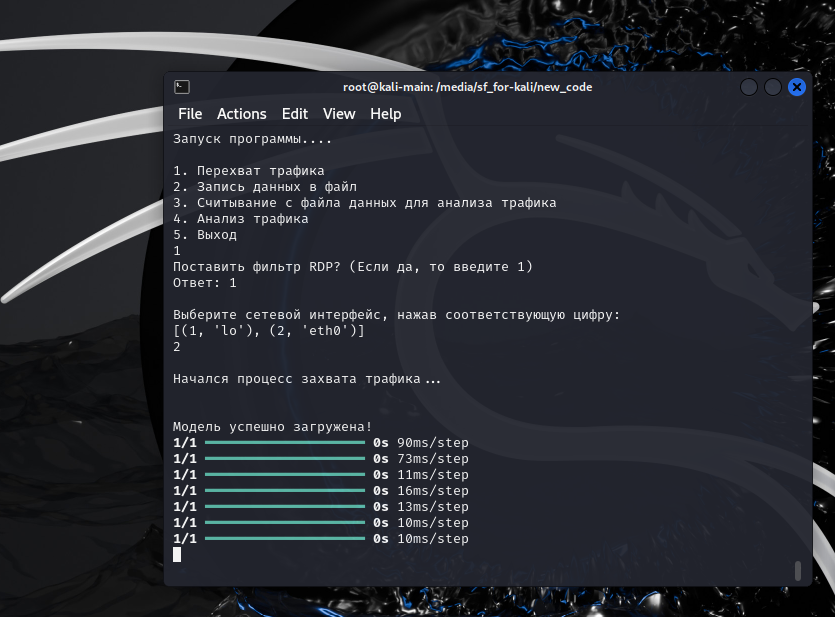
\includegraphics[width=0.9\textwidth]{pics/main-view.png}
  \caption{Запуск перехвата трафика с фильтром RDP}
  \label{main1}
\end{figure}


% На ВМ Kali был предварительно запущен HTTP-сервер, на котором хранилось несколько файлов разного размера, а также видео которое также можно посмотреть.
% Просмотр страницы HTTP-сервера совершался с другой ВМ типа Win. На Win совершались активные попытки скачивания большого файла с сервера. Из рисунка \ref{http1}
% видно, что ложных срабатываний за весь период активного взаимодействия с HTTP сервером не наблюдалось.

% \begin{figure}[H]
%   \centering
%   \includegraphics[width=0.9\textwidth]{pics/2http.png}
%   \caption{Состояние программы при HTTP-трафике}
%   \label{http1}
% \end{figure}


% Далее был рассмотрен еще один протокол прикладного уровня, а именно протокол FTP. Этот протокол полезен для загрузки и выгрузки файлов. Подключение осуществлялось 
% по протоколу FTP между Win и Kali. После успешной установки соединения пользователм были сделаны различные команды, после того как пользователь нашел большой файл, то
% он начал его скачивать, как показано на рисунке \ref{ftp1}.

% \begin{figure}[H]
%   \centering
%   \includegraphics[width=0.9\textwidth]{pics/3ftp.png}
%   \caption{Соединение по протоколу FTP}
%   \label{ftp1}
% \end{figure}

% После нескольких успешных попыток скачивания большого файла ложных срабатываний также не наблюдалось.


% \begin{figure}[H]
%   \centering
%   \includegraphics[width=0.9\textwidth]{pics/4ftp.png}
%   \caption{Состояние программы при FTP-трафике}
%   \label{ftp2}
% \end{figure}

% На следующих двух рисунках показаны графики одной из метрик. 



% \begin{figure}[H]
%   \centering
%   \includegraphics[width=0.9\textwidth]{pics/http-in-out.png}
%   \caption{График отношения объема входящего и исходящего трафиков (HTTP)}
%   \label{httpg1}
% \end{figure}

% Из второго графика следует, что при FTP-сессии клиент и сервер при отправке и при получении получают почти одинаковое 
% количество пакетов.


% \begin{figure}[H]
%   \centering
%   \includegraphics[width=0.9\textwidth]{pics/ftp-in-out.png}
%   \caption{График отношения объема входящего и исходящего трафиков (FTP)}
%   \label{ftpg1}
% \end{figure}


% На следующем рисунке показано уже подключение по RDP. Соединение устанавливается между Win (клиент) и Kali (сервер). 
% Стоит отметить, что для осуществления такого подключения на Kali запускался сервис XRDP, бесплатный протокол 
% удаленного доступа, основанный на протоколе RDP (Microsoft Remote Desktop). Из рисунка \ref{rdp1} видно, что программа
% нашла активную RDP-сессию. При подключении по RDP совершались движения мышкой и нажатия клавиш клавиатуры. Буквально после 30 секунд
% модель смогла определить RDP-трафик.

% \begin{figure}[H]
%   \centering
%   \includegraphics[width=0.9\textwidth]{pics/7rdp.png}
%   \caption{Состояние программы при RDP-трафике}
%   \label{rdp1}
% \end{figure}

% Также стоит рассмотреть следующий график, показанный на рисунке \ref{rdpg1}. Если сравнить RDP с протоколами HTTP и FTP по данной 
% метрике, то видно насколько их поведение различается.

% \begin{figure}[H]
%   \centering
%   \includegraphics[width=0.9\textwidth]{pics/rdp-in-out.png}
%   \caption{График отношения объема входящего и исходящего трафиков (RDP)}
%   \label{rdpg1}
% \end{figure}

% Далее был рассмотрен еще один протокол прикладного уровня -- SSH. На следующем рисунке показано состояние программы при активной работе
% с протоколом SSH.

% \begin{figure}[H]
%   \centering
%   \includegraphics[width=0.9\textwidth]{pics/5ssh.png}
%   \caption{Состояние программы при SSH-трафике}
%   \label{ssh1}
% \end{figure}


% Стоит отметить, что если исследовать графики, то поведение SSH и RDP достаточно похоже. Особенно если при подключении по SSH
% выполнять какие-либо непрерывные действия, например открыть большой файл и листать его строки. Если сравнить графики SSH и RDP по метрике
% отношения объема входящего и исходящего трафиков, то можно заметить некоторую схожесть

% \begin{figure}[H]
%   \centering
%   \includegraphics[width=0.9\textwidth]{pics/ssh-in-out.png}
%   \caption{График отношения объема входящего и исходящего трафиков (SSH)}
%   \label{sshg1}
% \end{figure}

% Однако, если смотреть по остальным признакам, как показано на следующих двух рисунках, то можно заметить небольшое различие в этих двух видах протоколов.

% \begin{figure}[H]
%   \centering
%   \includegraphics[width=0.9\textwidth]{pics/ssh-cnt-pack.png}
%   \caption{График отображения количества входящих пакетов (SSH)}
%   \label{sshg2}
% \end{figure}


% \begin{figure}[H]
%   \centering
%   \includegraphics[width=0.9\textwidth]{pics/rdp-cnt-pack.png}
%   \caption{График отображения количества входящих пакетов (RDP)}
%   \label{rdpg2}
% \end{figure}

На следующем рисунке показано подключение по RDP. В данном случае соединение устанавливается между Win (клиент) и Kali (сервер). 
Стоит отметить, что для осуществления такого подключения на Kali запускался сервис XRDP, бесплатный протокол 
удаленного доступа, основанный на протоколе RDP. Из рисунка \ref{rdp1} видно, что программа
нашла активную RDP-сессию.

\begin{figure}[H]
  \centering
  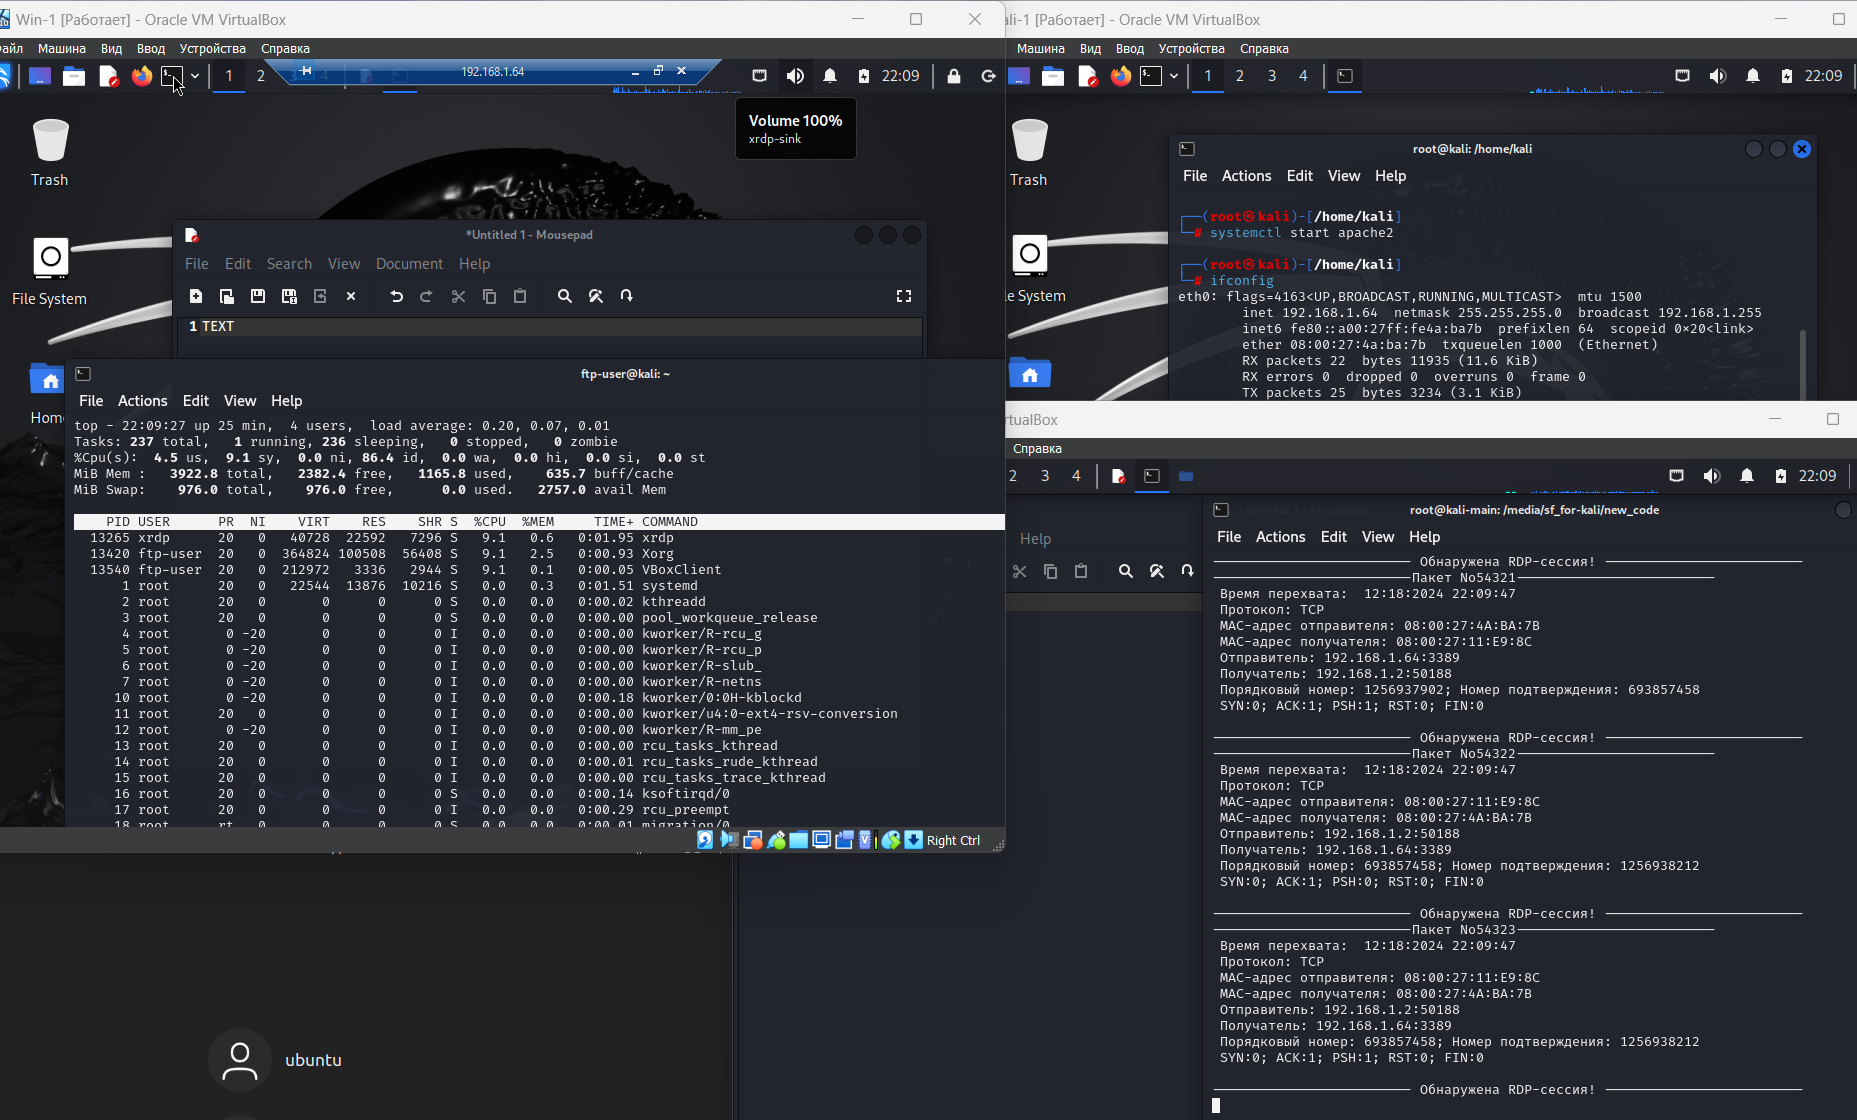
\includegraphics[width=1.0\textwidth]{pics/new1.png}
  \caption{Состояние программы при RDP-трафике}
  \label{rdp1}
\end{figure}

При подключении по RDP совершались движения мышкой и нажатия клавиш клавиатуры. Буквально после 30 секунд
модель смогла определить RDP-трафик. После завершения RDP-сессии проводилась работа с другими протоколами.

На ВМ Kali был предварительно запущен HTTP-сервер, на котором хранилось несколько файлов разного размера, а также 
видео которое также можно было посмотреть. Открытие страницы HTTP-сервера совершалось с другой ВМ Win. На Win 
совершались активные попытки скачивания большого файла с сервера и вместе с этим просматривалось видео. Из рисунка \ref{http1}
видно, что ложных срабатываний за весь период активного взаимодействия с HTTP сервером не наблюдалось.

\begin{figure}[H]
  \centering
  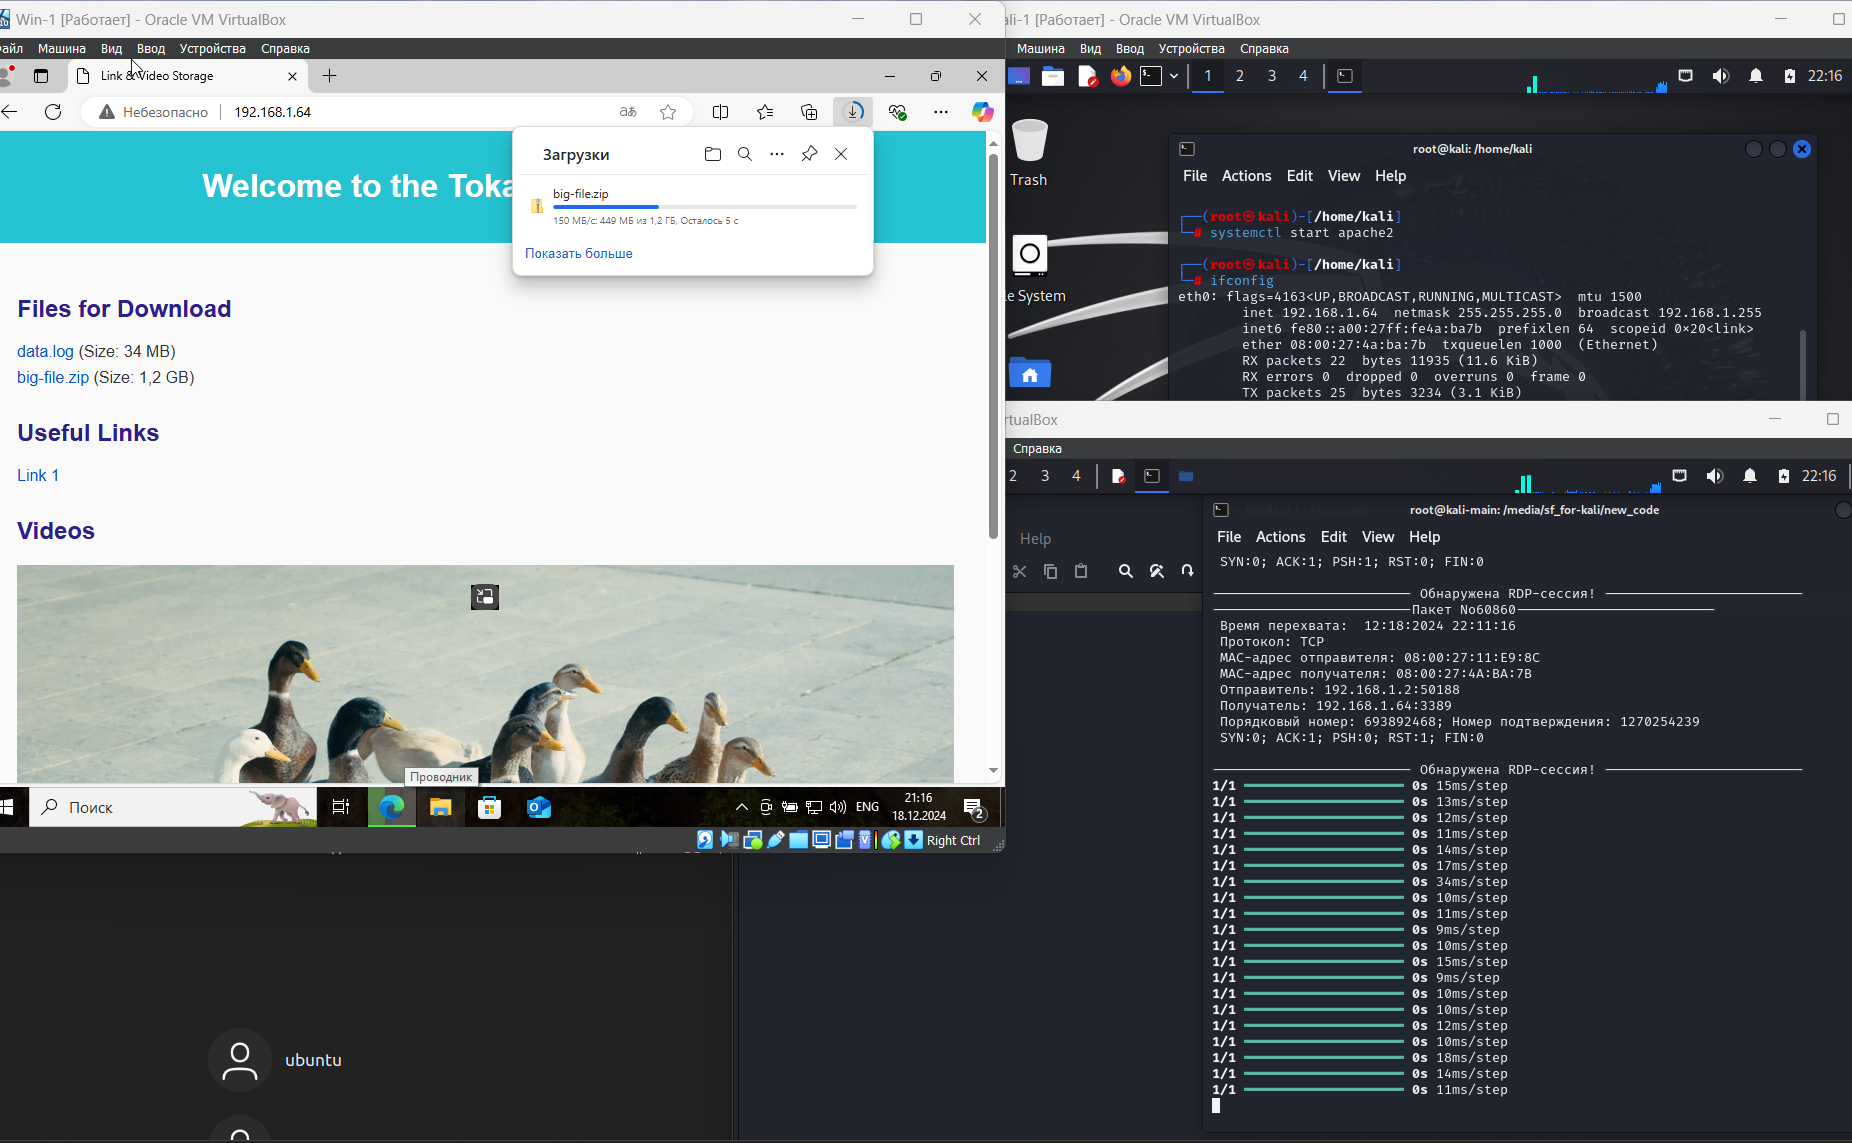
\includegraphics[width=1.0\textwidth]{pics/new2.png}
  \caption{Состояние программы при HTTP-трафике}
  \label{http1}
\end{figure}


Далее был рассмотрен еще один протокол прикладного уровня, а именно протокол FTP. Этот протокол полезен для загрузки и выгрузки файлов. Подключение осуществлялось 
по протоколу FTP между Win и Kali. После успешной установки соединения пользователем были сделаны различные команды, 
после того как пользователь нашел большой файл, то
он начал его скачивать, как показано на рисунке \ref{ftp1}.

\begin{figure}[H]
  \centering
  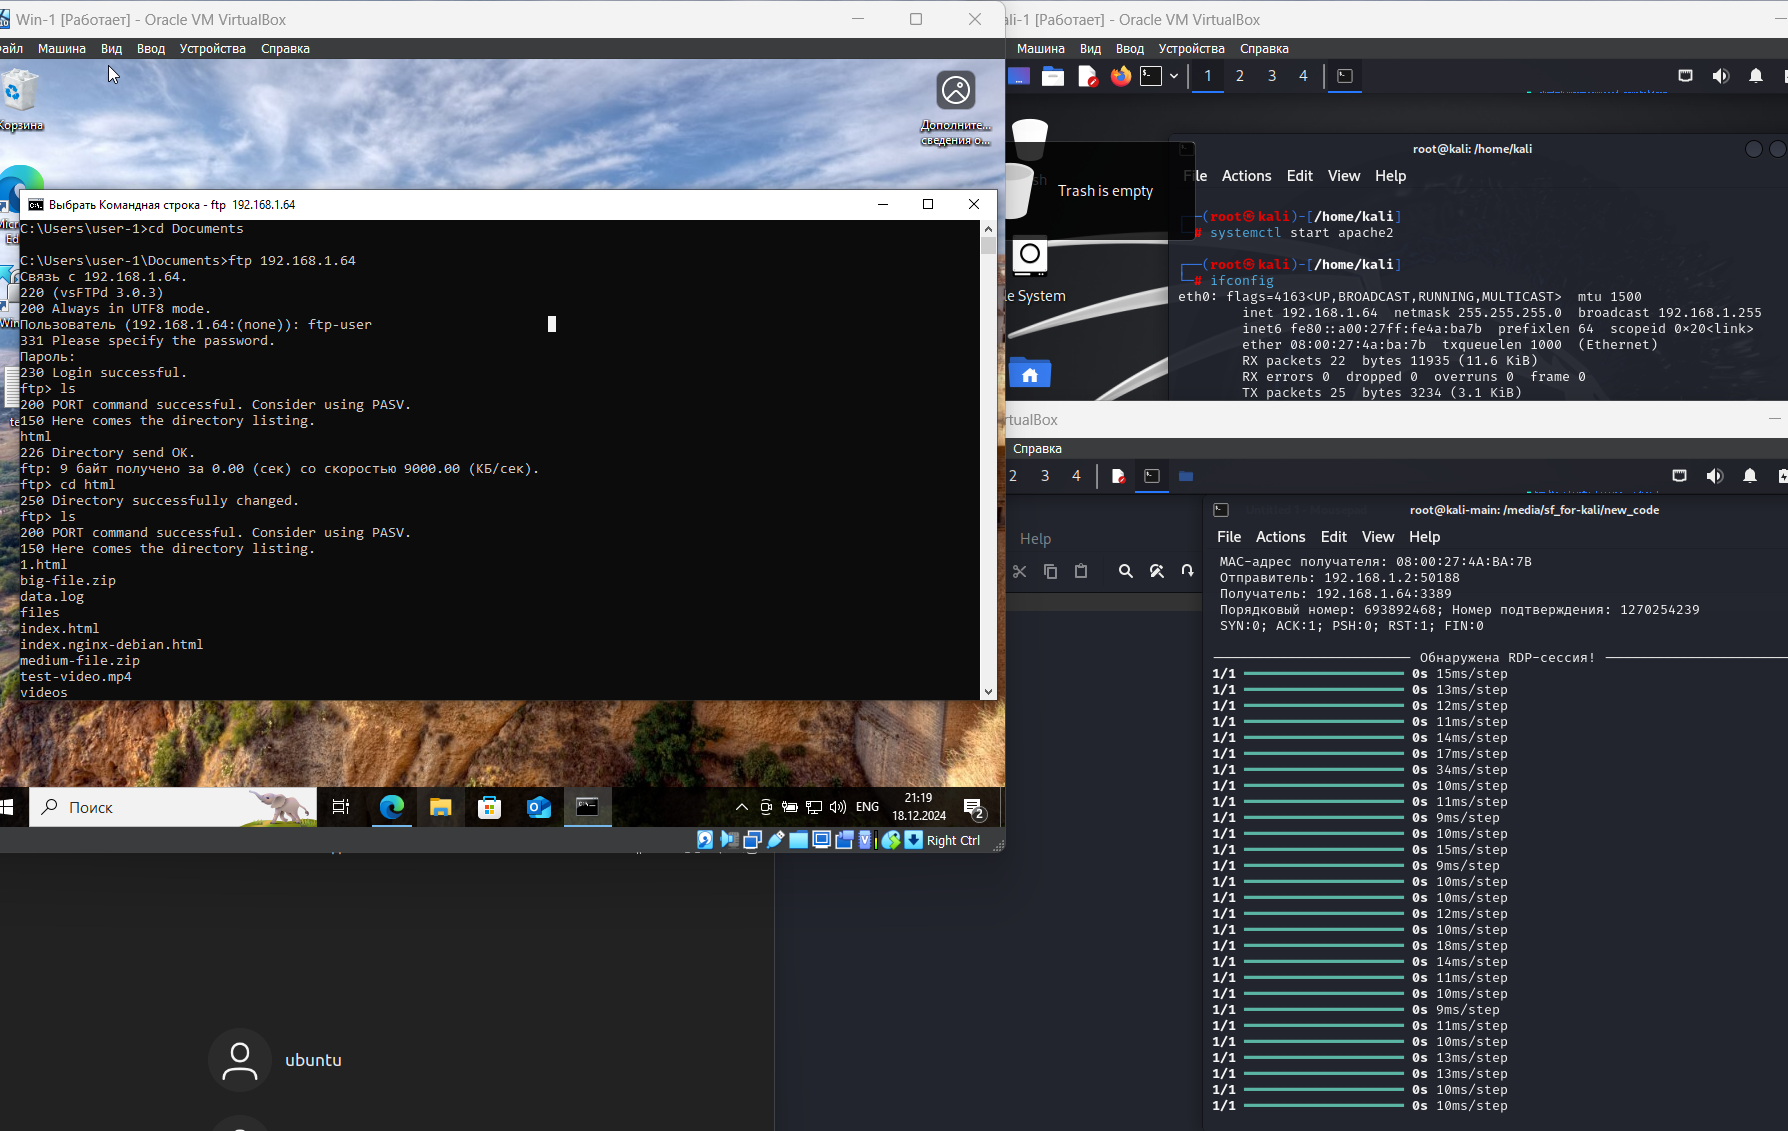
\includegraphics[width=1.0\textwidth]{pics/new3.png}
  \caption{Соединение по протоколу FTP}
  \label{ftp1}
\end{figure}

После нескольких успешных попыток скачивания большого файла ложных срабатываний также не наблюдалось.


\begin{figure}[H]
  \centering
  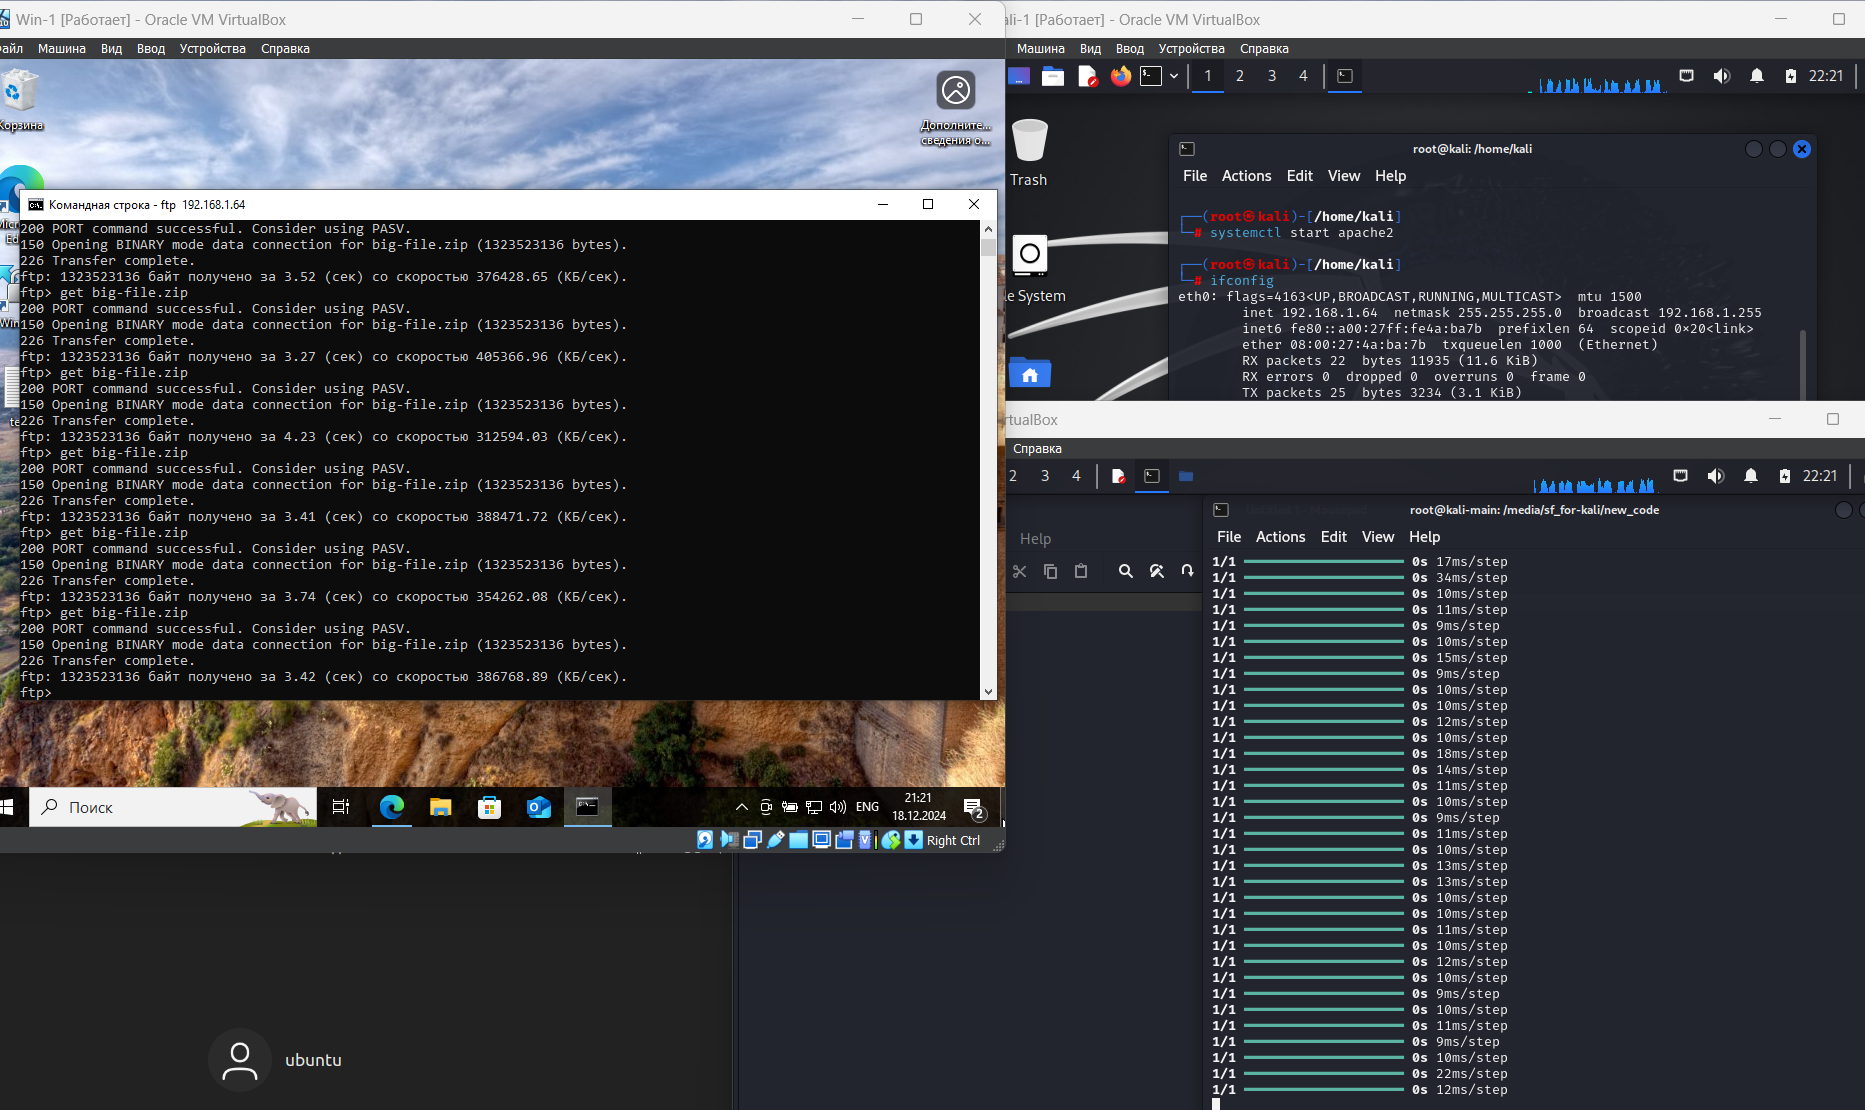
\includegraphics[width=1.0\textwidth]{pics/new4.png}
  \caption{Состояние программы при FTP-трафике}
  \label{ftp2}
\end{figure}

На следующих двух рисунках показаны графики одной из метрик. 



\begin{figure}[H]
  \centering
  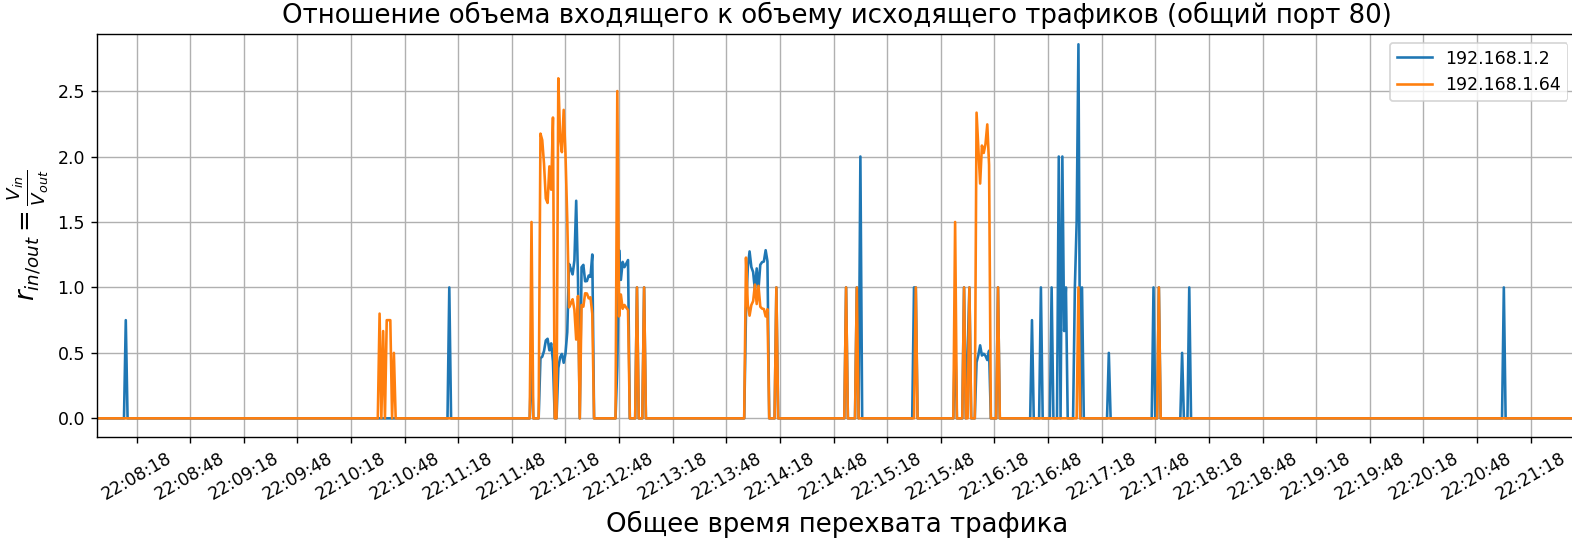
\includegraphics[width=1.0\textwidth]{pics/newhttp1.png}
  \caption{График отношения объема входящего и исходящего трафиков (HTTP)}
  \label{httpg1}
\end{figure}

Из второго графика следует, что при FTP-сессии клиент и сервер при отправке и при получении получают почти одинаковое 
количество пакетов.


\begin{figure}[H]
  \centering
  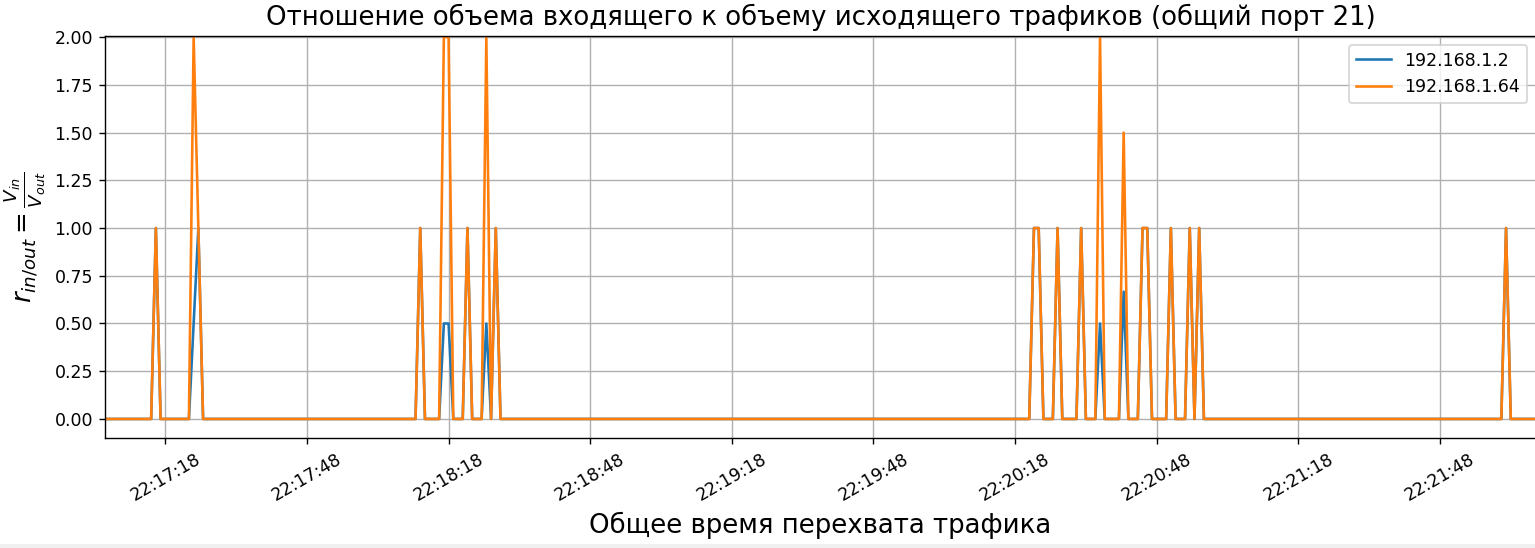
\includegraphics[width=1.0\textwidth]{pics/newftp1.png}
  \caption{График отношения объема входящего и исходящего трафиков (FTP)}
  \label{ftpg1}
\end{figure}

Для сравнения на рисунке \ref{rdpg1} показан следующий график.

\begin{figure}[H]
  \centering
  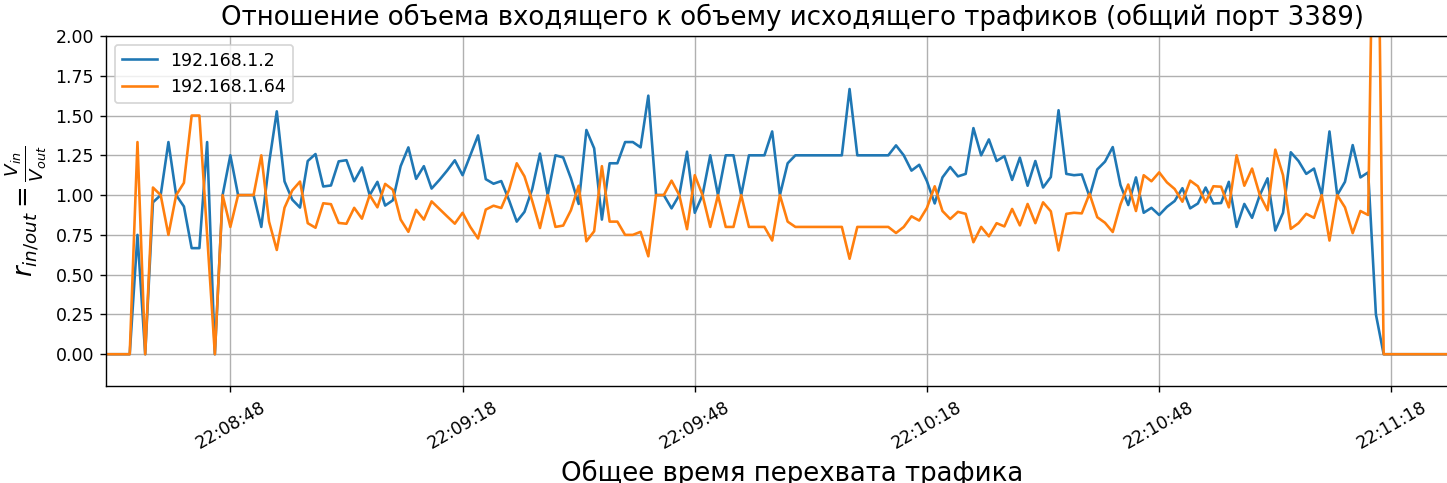
\includegraphics[width=1.0\textwidth]{pics/newrdp1.png}
  \caption{График отношения объема входящего и исходящего трафиков (RDP)}
  \label{rdpg1}
\end{figure}

Из рисунков \ref{httpg1} - \ref{rdpg1} видно, что по метрике отношения объемов входящего и исходящего трафиков поведение RDP различается
от поведений HTTP и FTP.

Далее был рассмотрен еще один протокол прикладного уровня -- SSH. На следующем рисунке показано состояние программы при активной работе
с протоколом SSH.

\begin{figure}[H]
  \centering
  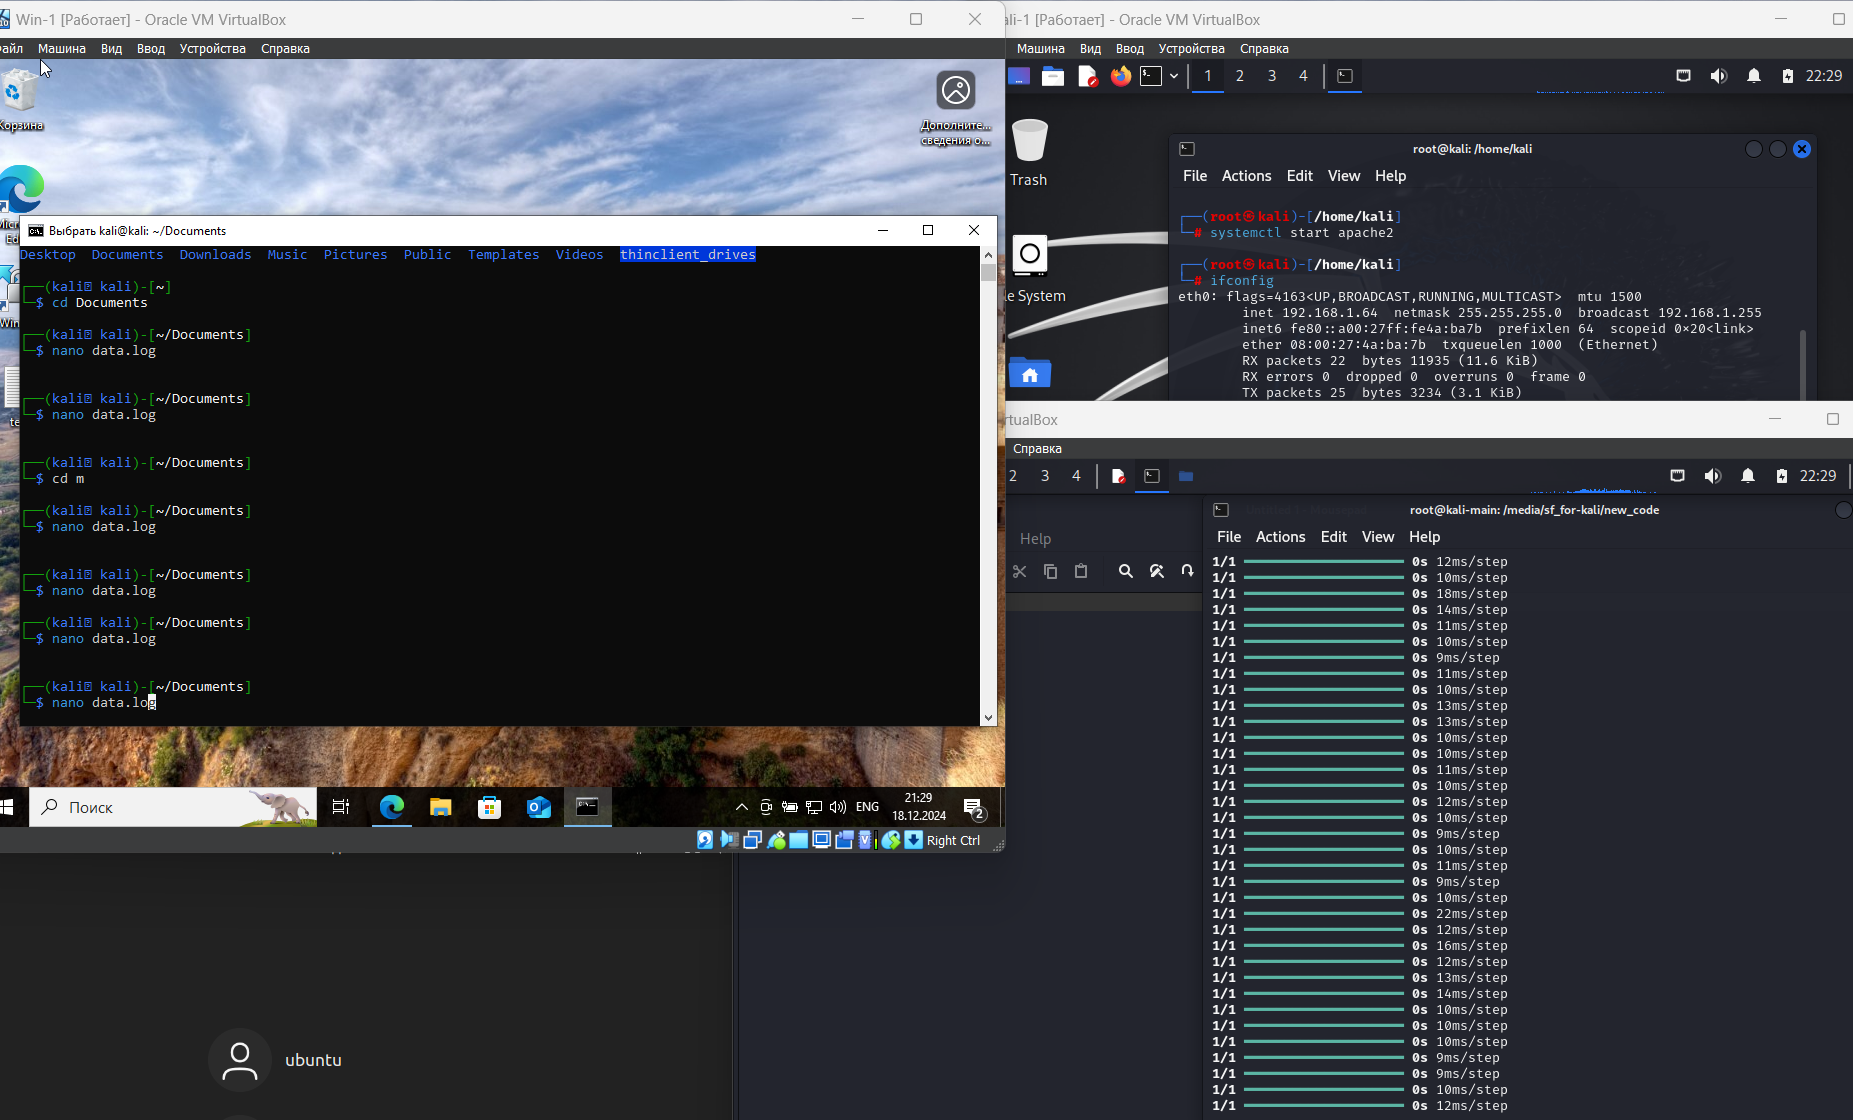
\includegraphics[width=1.0\textwidth]{pics/new5.png}
  \caption{Состояние программы при SSH-трафике}
  \label{ssh1}
\end{figure}


Стоит отметить, что если исследовать графики, показанные на рисунках \ref{rdpg1} и \ref{sshg1}, то поведение SSH и RDP достаточно похоже. 
Особенно если при подключении по SSH выполнять какие-либо непрерывные действия, например открыть большой файл и листать его строки. 
Если сравнить графики SSH и RDP по метрике отношения объемов входящего и исходящего трафиков, то можно заметить некоторую схожесть.

\begin{figure}[H]
  \centering
  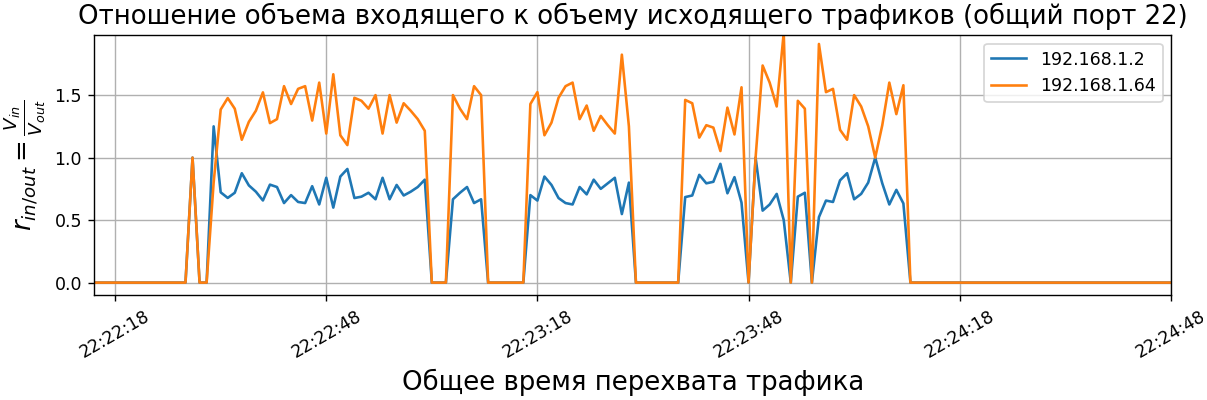
\includegraphics[width=0.9\textwidth]{pics/newssh1.png}
  \caption{График отношения объема входящего и исходящего трафиков (SSH)}
  \label{sshg1}
\end{figure}

Однако, если смотреть по другим признакам, как показано на следующих двух рисунках, то можно заметить небольшое различие в этих двух видах протоколов.

\begin{figure}[H]
  \centering
  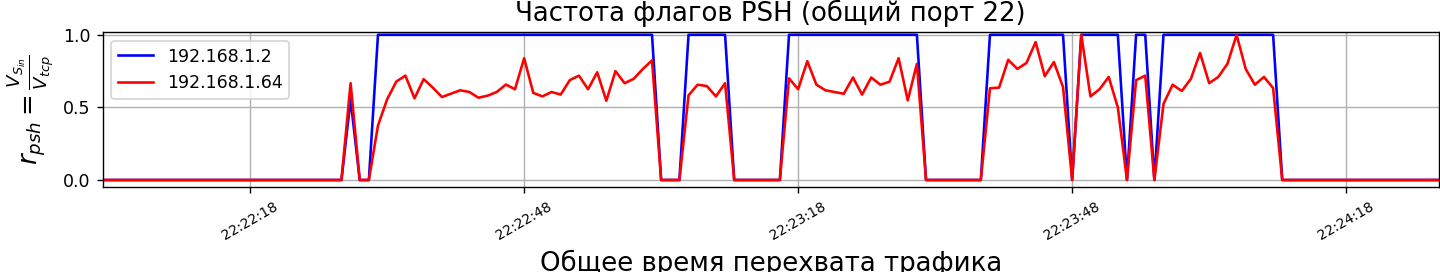
\includegraphics[width=0.9\textwidth]{pics/newssh2.png}
  \caption{График отображения количества входящих пакетов (SSH)}
  \label{sshg2}
\end{figure}

Частота флагов PSH является одним из ключевых признаков, по которым можно сформировать небольшое представление о поведении протоколов. Особенно, если это касается
протокола RDP, так как этот протокол активно использует флаги PSH для передачи данных. Флаги PSH сигнализируют о том, что данные должны быть немедленно 
переданы приложению, что важно для обеспечения быстрой реакции интерфейса пользователя. В данном случае из рисунка \ref{rdpg2} видно, как клиент с IP-адресом 192.168.1.2
активно получает входящие TCP-пакеты с установленным флагом PSH от сервера.

\begin{figure}[H]
  \centering
  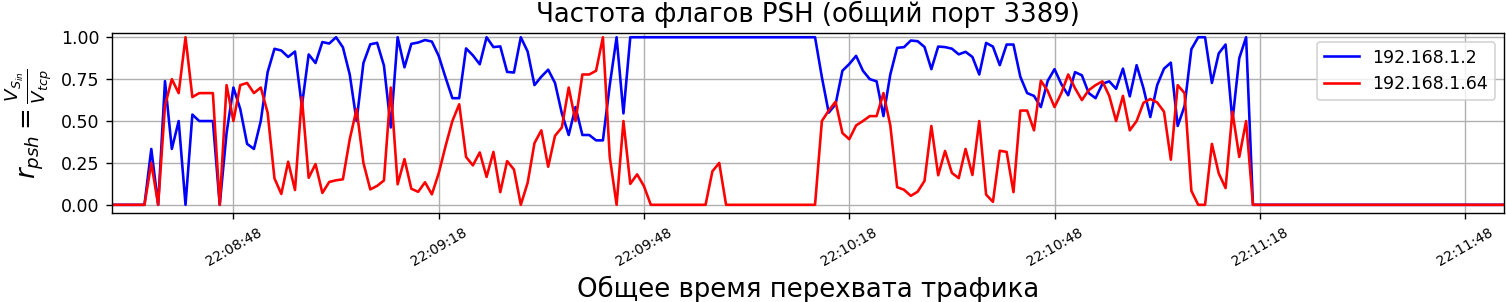
\includegraphics[width=0.9\textwidth]{pics/newrdp2.png}
  \caption{График отображения количества входящих пакетов (RDP)}
  \label{rdpg2}
\end{figure}



Исходя из рассмотренных рисунков программа способна по определенным признакам различать один тип трафика от другого и демонстрировать 
надежность анализа даже в сложных случаях, когда различия между протоколами минимальны. Таким образом, программа может быть использована 
как для исследовательских целей, так и для практического применения в области сетевой безопасности.

\subsubsection{Сравнительный анализ альтернативных программ удаленного доступа}

Каждый сетевой протокол разработан для решения специфических задач, используя уникальные технологии. Тем не 
менее существуют протоколы, которые имеют схожую структуру и поведение. В рамках данной работы важно также 
изучить альтернативные программы удаленного доступа, такие как Ammyy Admin, Remmina и RAdmin. Основной задачей 
этого раздела является демонстрация работы программы при использовании этих приложений.

Прежде чем перейти к анализу альтернативных программ, необходимо рассмотреть случай изменения стандартного порта для RDP. На виртуальной машине с 
операционной системой Windows порт по умолчанию для RDP-соединения был изменен с 3389 на 53389 \cite{rdpport}. На рисунке \ref{rdp2} показан процесс 
установления RDP-соединения, а также вывод программы с информацией о пакетах этой сессии. Программа успешно идентифицировала RDP-сессию, 
что подтверждает её способность работать независимо от номера порта. Это особенно важно, так как использование анализа, основанного только 
на портах, является ненадежным методом, как упоминалось ранее.

\begin{figure}[H]
  \centering
  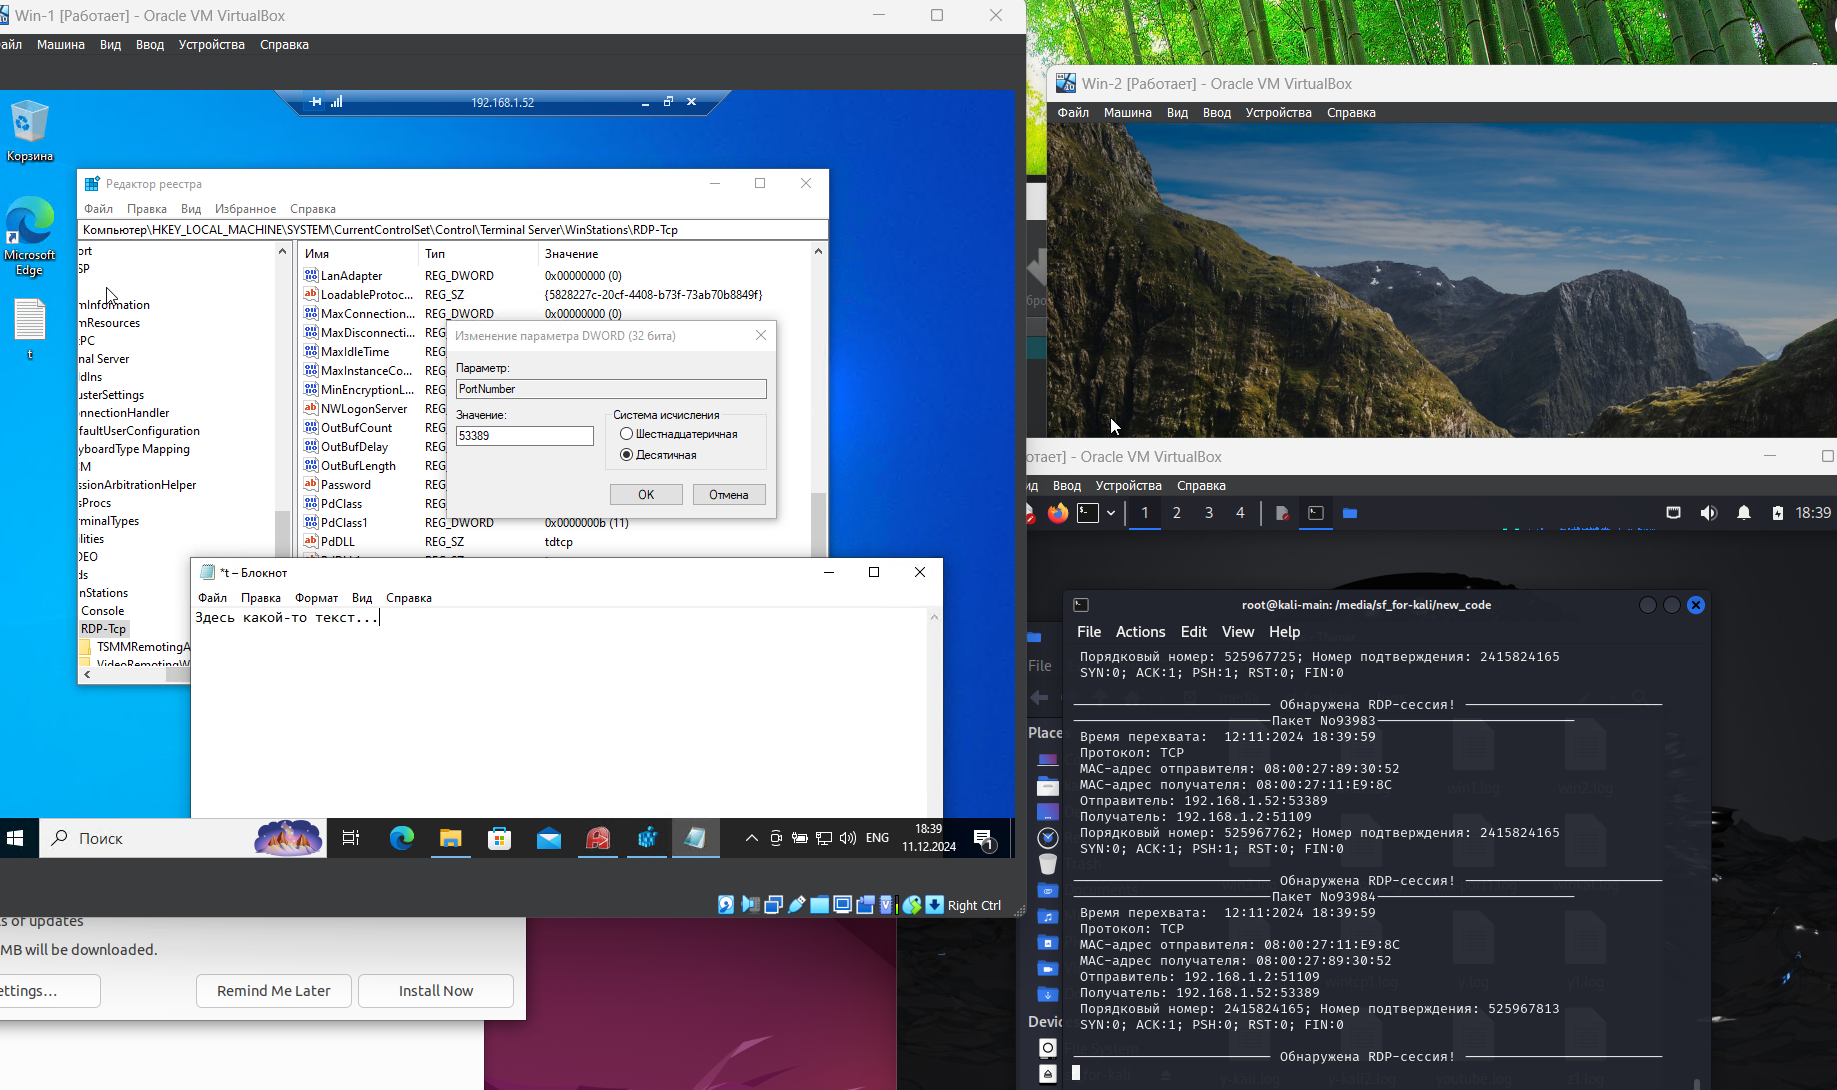
\includegraphics[width=1.0\textwidth]{pics/8rdp.png}
  \caption{Состояние программы при RDP-трафике (смена порта)}
  \label{rdp2}
\end{figure}

Ammyy Admin -- это программа удаленного доступа и администрирования, разработанная компанией Ammyy Group. Она 
позволяет пользователям получать удаленный доступ к компьютерам и серверам через интернет и управлять ими 
в реальном времени. На следующем рисунке показано подключение с помощью Ammyy Admin между двумя ВМ операционной системы Windows. 
Так как данное приложение поддерживает протокол RDP, то программа смогла распознать признаки RDP-сессии.


\begin{figure}[H]
  \centering
  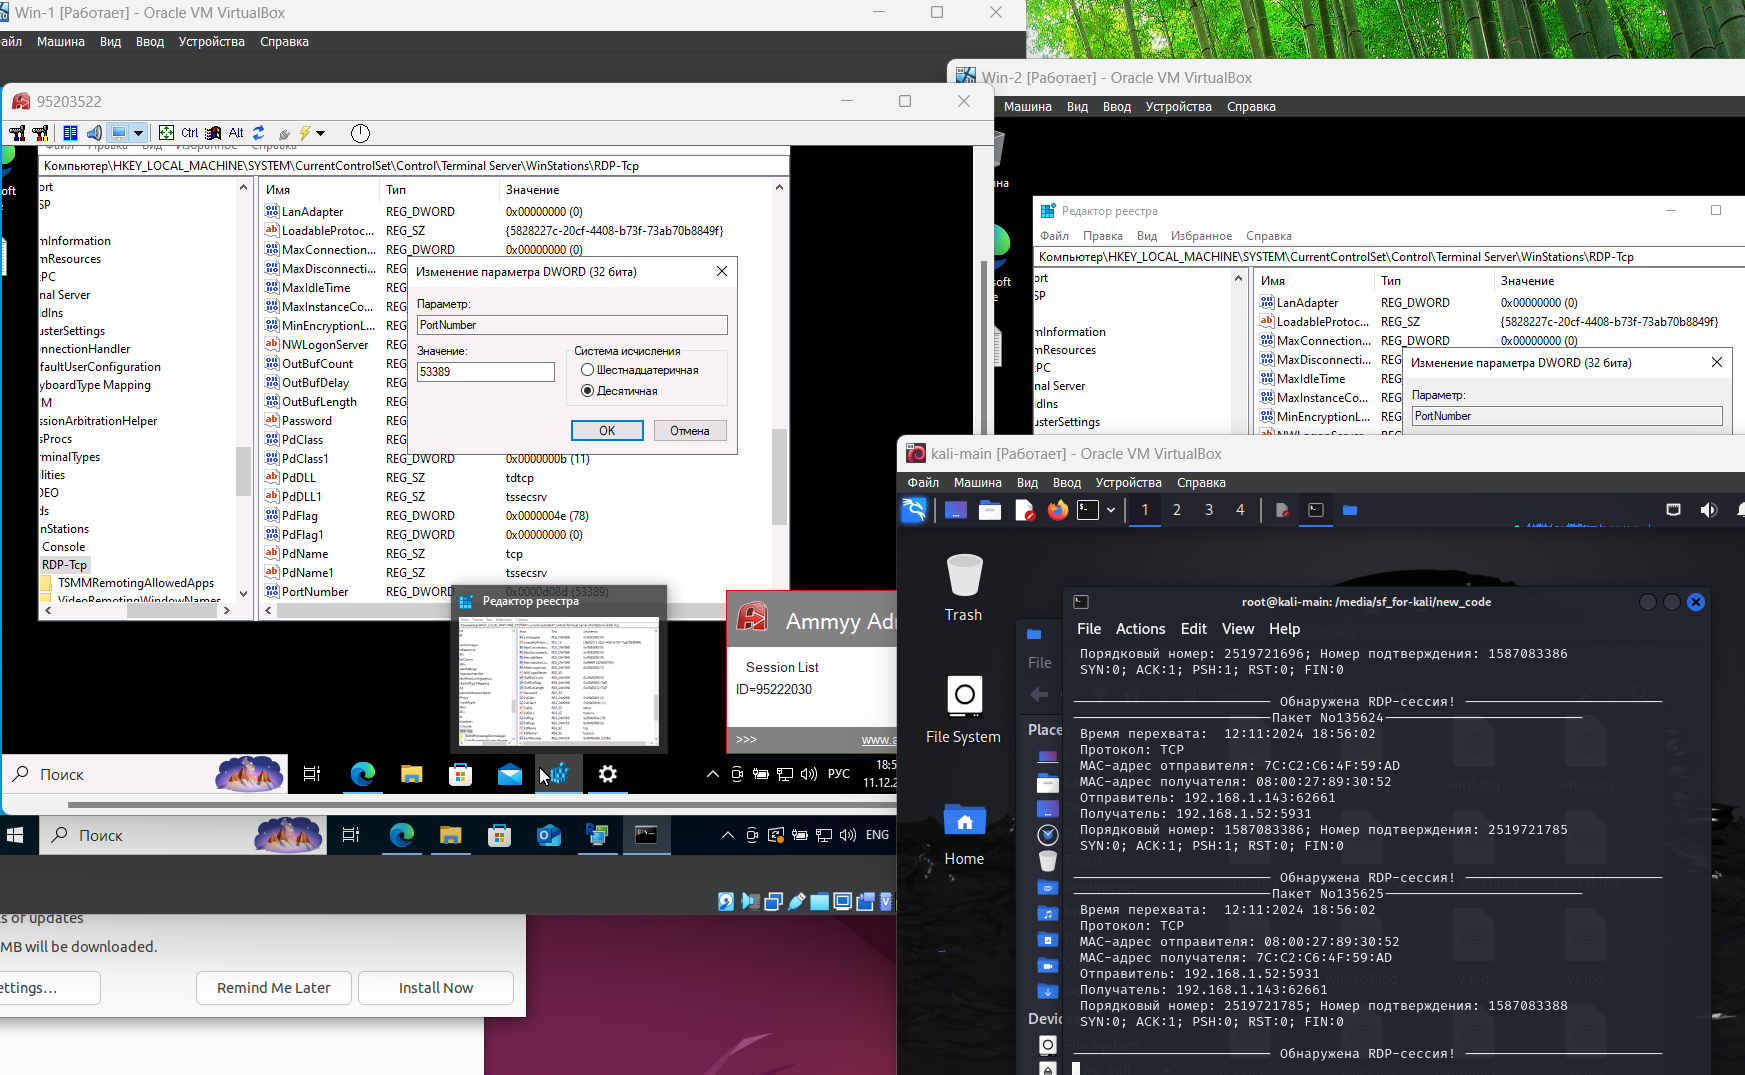
\includegraphics[width=1.0\textwidth]{pics/9ammyy.png}
  \caption{Состояние программы при RDP-трафике (использование Ammyy Admin)}
  \label{ammyy1}
\end{figure}

Аналогичное поведение наблюдается при использовании Remmina, бесплатной программы для удаленного доступа, ориентированной 
на пользователей операционной системы Linux. На рисунке \ref{remmina1} видно, как было установлено подключение между Ubuntu (клиента) и Win (сервера).  

\begin{figure}[H]
  \centering
  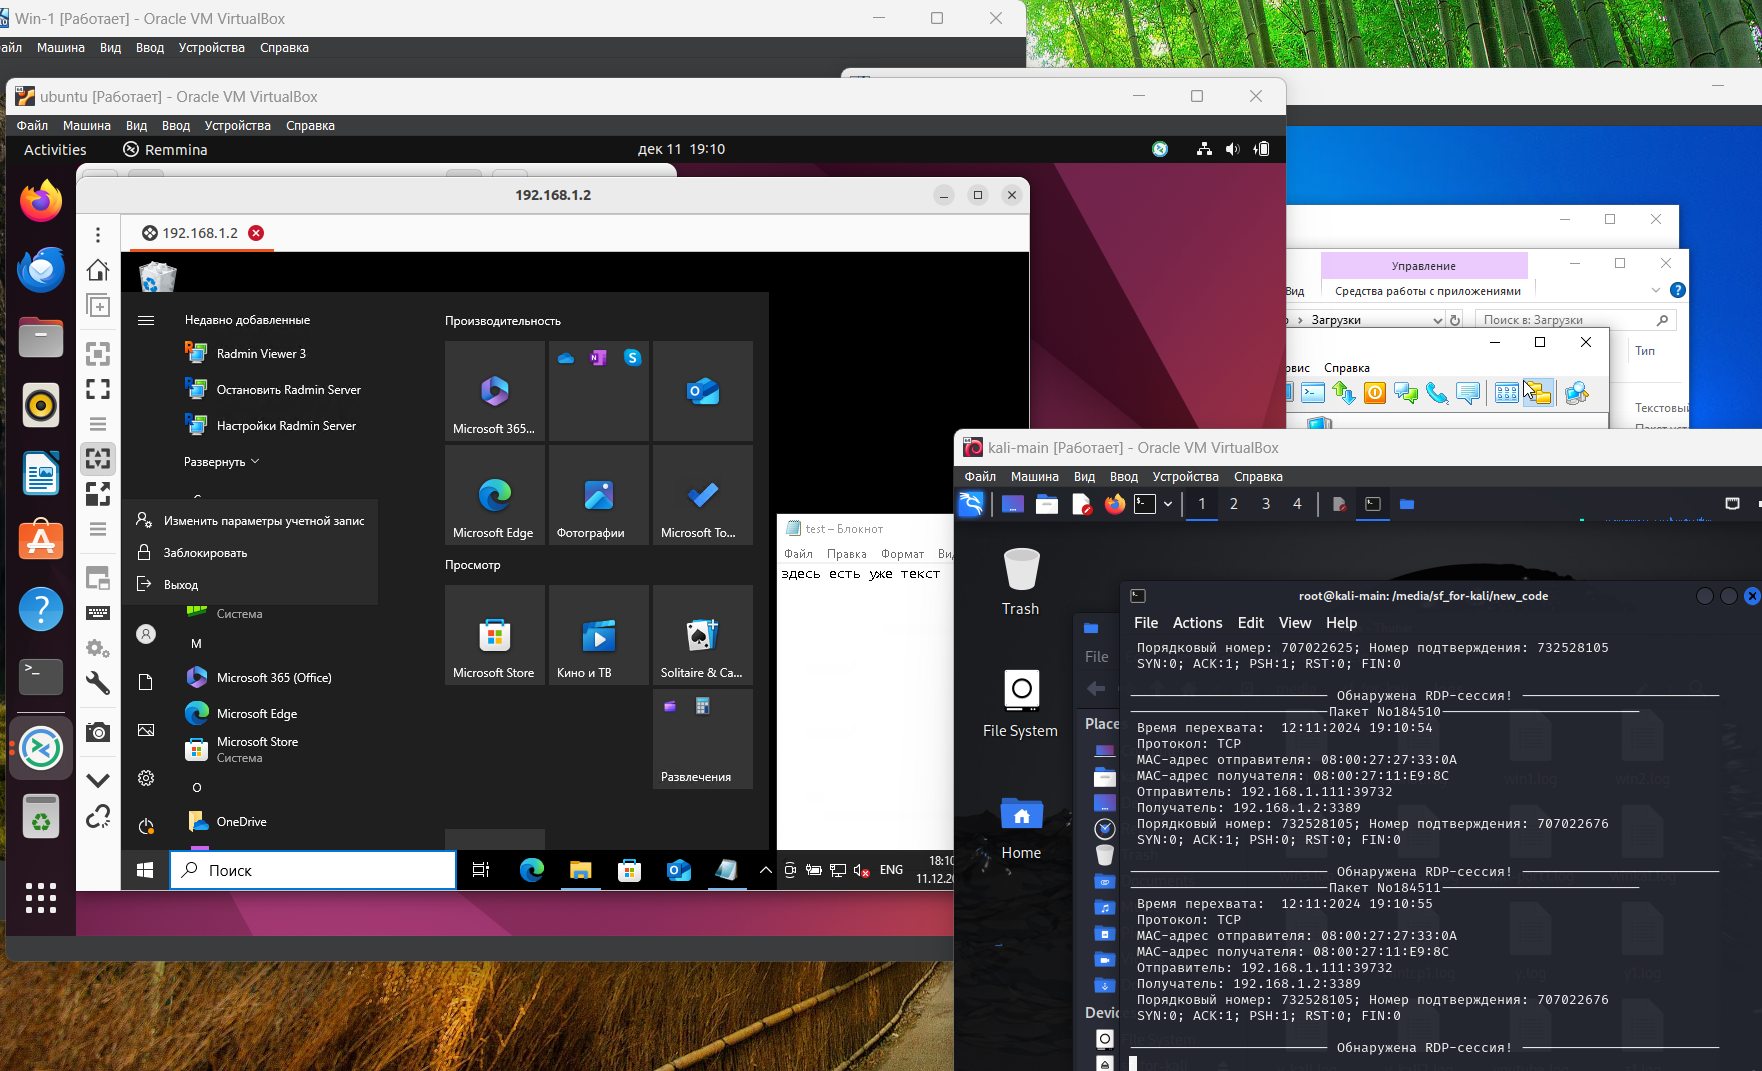
\includegraphics[width=1.0\textwidth]{pics/10remmina.png}
  \caption{Состояние программы при RDP-трафике (использование Remmina)}
  \label{remmina1}
\end{figure}


RAdmin -- это программа удалённого администрирования для платформ Windows, разработанная компанией Famatech. Она 
является одной из альтернатив подключения к удаленному рабочему столу. Исходя из следующего рисунка, подключение с помощью RAdmin
также распознается программой.


\begin{figure}[H]
  \centering
  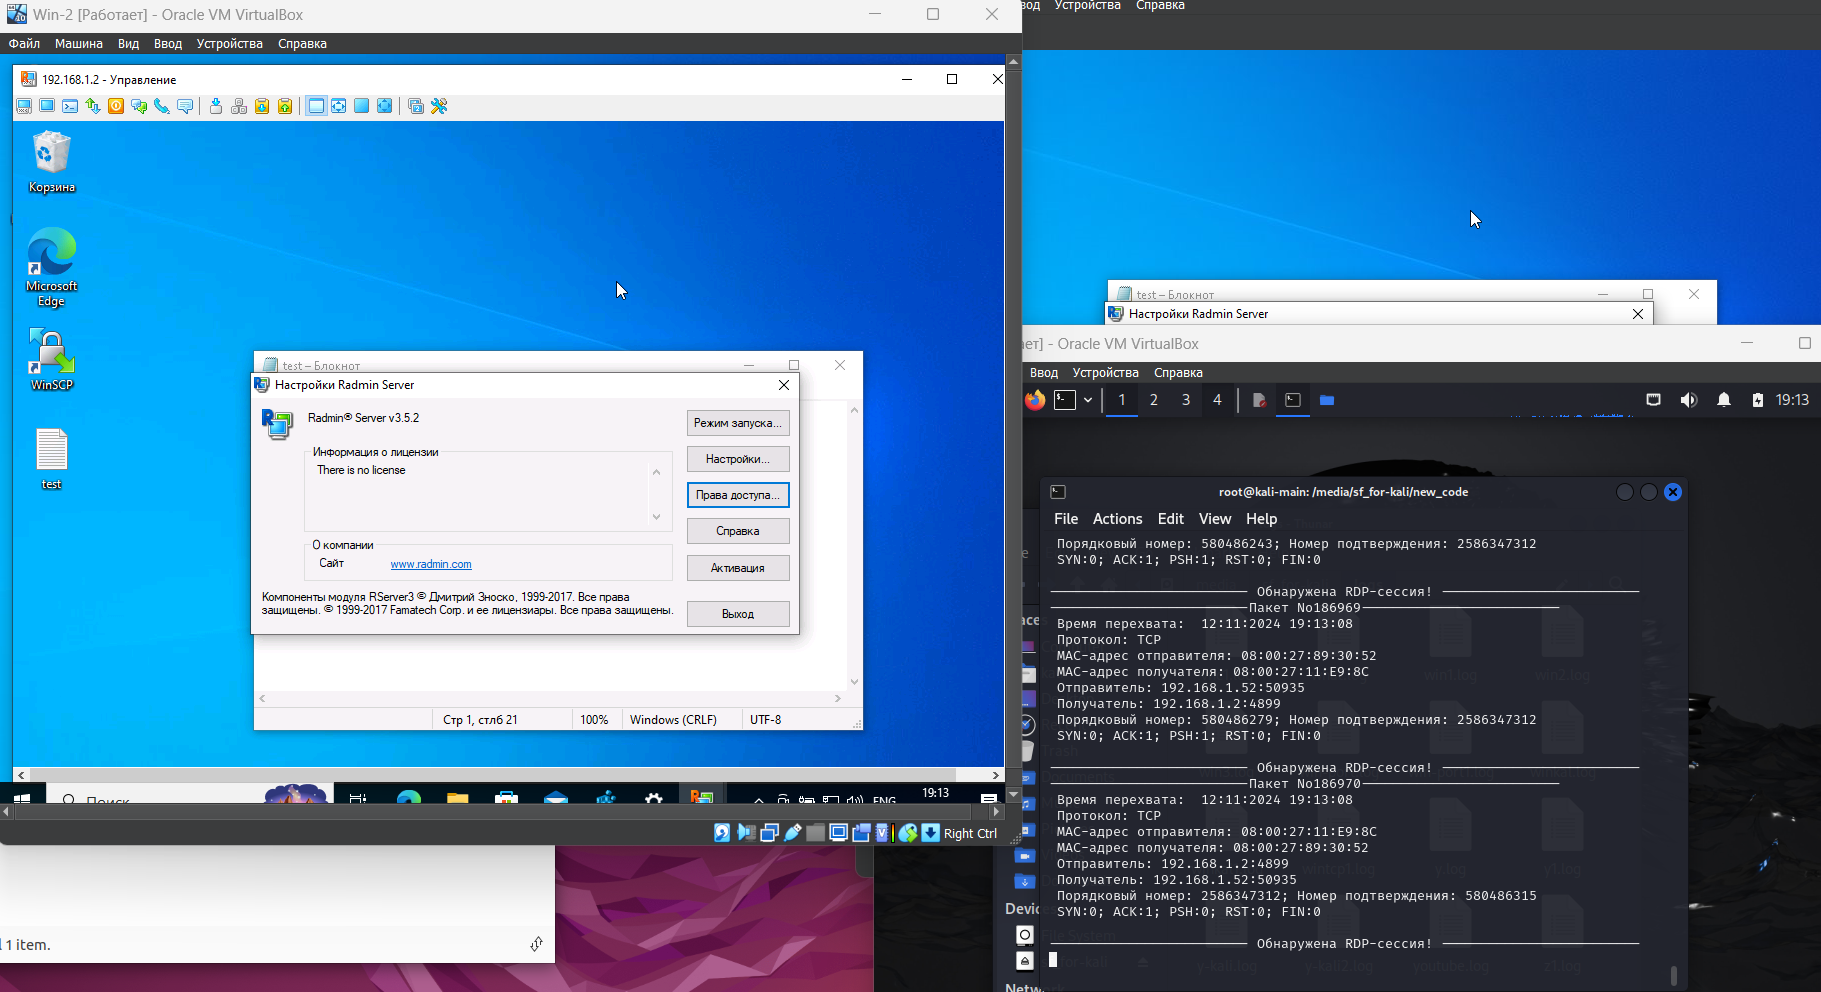
\includegraphics[width=1.0\textwidth]{pics/11radmin.png}
  \caption{Состояние программы использовании RAdmin}
  \label{radmin1}
\end{figure}

Стоит отметить, что первые попытки работы с такими сервисами, как Ammyy Admin, Remmina и RAdmin, приводили к 
идентификации их трафика как RDP. Таким образом, разработанная программа способна распознавать трафик альтернативных 
приложений как RDP благодаря их схожести в поведении. Это указывает на универсальность подхода, позволяющего 
идентифицировать не только известные, но и неизвестные сервисы с аналогичной структурой передачи данных. 
Такой результат особенно ценен для задач мониторинга и анализа сетевого трафика, где важна способность 
адаптироваться к изменениям и новым угрозам.


% \subsection{Точность и производительность модели}

\conclusion

В данной работе была разработана программа для анализа сетевого трафика с использованием модели нейронной сети LSTM, 
предназначенная для выявления RDP-сессий. Решение позволяет идентифицировать трафик удаленного рабочего стола даже при его шифровании, основываясь 
на анализе временных характеристик пакетов и побочной информации, что подчеркивает актуальность и практическую значимость предложенного подхода.  

С помощью данной модели программа получила способность идентифицировать трафик, схожий с RDP, что 
позволяет применять её для обнаружения альтернативных приложений удалённого доступа. Программа работает в режиме 
реального времени, что обеспечивает её практическую применимость для задач мониторинга корпоративных и частных сетей.

Полученные результаты подчеркивают перспективы использования нейронных сетей для задач сетевой безопасности. 
В дальнейших исследованиях можно рассмотреть другие архитектуры нейронных сетей для выявления RDP-трафика с целью повышения точности 
классификации и снижения вычислительных затрат. Также важно обратить внимание на поиск и внедрение дополнительных статистических методов анализа 
сетевого трафика. Текущая реализация не является пределом совершенства, и ее можно улучшить за счет добавления новых метрик, что позволит более полно 
охватить различные аспекты сетевых взаимодействий и сделать анализ более точным и надежным.

\begin{thebibliography}{25}
    \bibitem{lib2}
    Карачанская, Е. В. Метод выявления аномалий сетевого трафика, основанный на его самоподобной структуре / Е.В. Карачанская, Н.И. Соседова // 
    Безопасность информационных технологий. - 2019. - Т. 26. - № 1. - С. 98-110.
    \bibitem{lib1}
    Фаткиева, Р. Р. Разработка метрик для обнаружения атак на основе анализа сетевого трафика / Р. Р. Фаткиева // Вестник Бурятского государственного университета. 
    Математика, информатика. - 2013. - № 9. - С. 81-86.
    \bibitem{lib3}
    Шелухин, О. И. Обнаружение аномальных вторжений в компьютерные сети статистическими методами / О. И. Шелухин, А. С. Филинова, А. В. Васина // T-Comm: 
    Телекоммуникации и транспорт. - 2015. - Т. 9. - № 10. - С. 42-49.
    % \bibitem{2}
    % Alexey Удалённый рабочий стол RDP: как включить и как подключиться по RDP [Электронный ресурс] : настройка удаленного рабочего стола RDP. -- URL: https://hackware.ru/?p=11835\#11 (дата обращения: 31.03.2023). -- Загл. с экрана. -- Яз. рус.
    \bibitem{rdp22}
    Liang, H. Understanding the Remote Desktop Protocol (RDP) / H. Liang, L. Chen // [Электронный ресурс] : описание протокола удаленного рабочего стола RDP. - 
    URL: \url{https://learn.microsoft.com/en-us/troubleshoot/windows-server/remote/understanding-remote-desktop-protocol} (дата обращения: 30.11.2024). - Загл. с экрана. - Яз. англ.
    \bibitem{stack}
    Кручинин, С. В. Стеки сетевых технологий TCP/IP и OSI/ISO / С. В. Кручинин // Вопросы науки. - 2015. - Т. 3. - С. 145-147.
    \bibitem{osi-model}
    Maintenance script Модель OSI [Электронный ресурс] : описание модели OSI. - Университет ИТМО. - URL: \url{http://neerc.ifmo.ru/wiki/index.php?title=OSI_Model}
    (дата обращения: 30.11.2024). - Загл. с экрана. - Яз. рус.
    \bibitem{tcpip}
    Rodriguez, A. TCP/IP Tutorial and Technical overview / A. Rodriguez, J. Gatrell, J. Karas // [Электронный ресурс] : описание стандарта компютерных коммуникаций TCP/IP. -
    URL: \url{https://citeseerx.ist.psu.edu/document?repid=rep1&type=pdf&doi=738cba440ca5537f98da948144bd5e7fa4243337} (дата обращения: 01.12.2024). - Загл. с экрана. - Яз. англ.
    \bibitem{winsize}
    Liang, H. Описание функций Windows TCP /  H. Liang, L. Chen, A. Li // [Электронный ресурс] : описание параметров TCP-заголовка . - URL: 
    \url{https://learn.microsoft.com/ru-ru/troubleshoot/windows-server/networking/description-tcp-features} (дата обращения: 01.12.2024). - Загл. с экрана. -  Яз. рус.
    \bibitem{tcpflags}
    KeyCDN TCP flags [Электронный ресурс] : описание TCP-флагов. - proinity LLC 2023. - URL: \url{https://www.keycdn.com/support/tcp-flags\#:$\sim$:text=ACK}
    (дата обращения: 01.12.2024). - Загл. с экрана. -  Яз. англ.
    \bibitem{udpseg}
    Remote Desktop Protocol: UDP Transport Extension [Электронный ресурс] : описание подключения к удаленному рабочему столу по протоколу UDP. - Microsoft 2024. - 
    \url{https://learn.microsoft.com/en-us/openspecs/windows_protocols/ms-rdpeudp/2744a3ee-04fb-407b-a9e3-b3b2ded422b1} (дата обращения: 07.12.2024). - Загл. с экрана. -  Яз. англ.
    \bibitem{lib4}
    Татарникова, Т. М. Статистические методы исследования сетевого трафика // Информационно-управляющие системы. - 2018. - №. 5 (96). - С. 35-43.
    \bibitem{dev0}
    Киреева, Н. В Исследование трафика локальной сети посредством сетевого анализатора <<Wireshark>> [Электронный ресурс] : методическая разработка к лабораторной работе / Н. В. Киреева, В.П. Зайкин, Н. Н. Васин // Поволжский государственный университет телекоммуникаций и информатики, Самара, 2010. - URL: http://ib.psuti.ru/content/metod/методическиеWireshark.pdf (дата обращения 08.12.2024). - Загл. с экрана. - Яз. рус.
    \bibitem{grad}
    Проблемы нейронных сетей [Электронный ресурс] : описание взрывающегося и затухающего градиента. - Университет ИТМО. - URL: https://neerc.ifmo.ru/wiki/index.php?title=Проблемы_нейронных_сетей (дата обращения: 08.12.2024). - Загл. с экрана. -  Яз. рус.
    \bibitem{nn}
    Созыкин, А. В. Обзор методов обучения глубоких нейронных сетей / А. В. Созыкин // Вестник ЮУрГУ. Серия: Вычислительная математика и информатика. 2017. - Т. 6. - № 3. - С. 28-59.
    \bibitem{keras}
    Ketkar, N. Introduction to keras / N. Ketkar // Deep learning with python: a hands-on introduction. - 2017. - С. 97-111.
    \bibitem{keras2}
    Dogo, E. M. A comparative analysis of gradient descent-based optimization algorithms on convolutional neural networks / E. M. Dogo, O. J. Afolabi // 
    2018 international conference on computational techniques, electronics and mechanical systems (CTEMS). - 2018. - С. 92-99.
    \bibitem{nn2}
    Бабушкина, Н. Е. Выбор функции активации нейронной сети в зависимости от условий задачи / Н. Е. Бабушкина, А. А. Рачев // Инновационные технологии в 
    машиностроении, образовании и экономике. - 2020. - Т. 27. - №. 2. - С. 12-15.
    \bibitem{lstm1}
    Schmidhuber, J. Long short-term memory / S. Hochreiter, J. Schmidhuber // Neural Comput. - 1997. - Т. 9. - №. 8. - С. 1735-1780.
    \bibitem{lstm2}
    Olah, C. Understanding LSTM Networks / C. Olah // Colah's Blog. - 2015. - Сведения доступны также по Интернет: https://colah.github.io/posts/2015-08-Understanding-LSTMs/ (дата обращения: 09.12.2024). - Загл. с экрана. - Яз. англ.
    % \bibitem{socket1}
    % The Python Standard Library Socket - Low-level networking interface [Электронный ресурс] : описание методов библиотеки socket. - Python Software Foundation 2001 - 2024. - URL: https://docs.python.org/3/library/socket.html (дата обращения: 15.12.2024). - Загл. с экрана. - Яз. англ.
    % \bibitem{session}
    % How Terminal Services Works [Электронный ресурс] : описание службы терминалов удаленного рабочего стола. -- Microsoft 2023. -- URL:  https://learn.microsoft.com/en-us/previous-versions/windows/it-pro/windows-server-2003/cc755399(v=ws.10)?redirectedfrom=MSDN (дата обращения: 14.04.2023). -- Загл. с экрана. -- Яз. англ.
    % \bibitem{remmina11}
    % Antenore Gatta The fast, stable, and always free Linux RDP client [Электронный ресурс] : подключение по RDP с помощью приложения Remmina. -- URL: https://www.remmina.org/remmina-rdp/ (дата обращения: 15.12.2024). -- Загл. с экрана. -- Яз.  англ.
    \bibitem{rdpport}
    Jenks, A. Change the listening port for Remote Desktop on your computer / A. Jenks, S. Manheim, H. Lohr // [Электронный ресурс] : изменение порта прослушивания для RDP. - Microsoft, 2024. - URL: \url{https://learn.microsoft.com/ru-ru/windows-server/remote/remote-desktop-services/clients/change-listening-port} (дата обращения: 15.12.2024). - Загл. с экрана. - Яз. англ.
    \bibitem{nn3}
    Гафаров, Ф. М. Искусственные нейронные сети и приложения: учеб пособие / Ф. М. Гафаров, А. Ф. Галимянов. - Казань: Изд-во Казан. ун-та. - 2018. - 121 с.
    \bibitem{lib5}
    Скатков, А. В. Сравнительный анализ методов обнаружения изменений состояний сетевого трафика / А. В. Скатков, А. А. Брюховецкий, Ю. Е. Шишкин //
    Автоматизация и приборостроение: проблемы, решения. - 2016. - С. 14-15.

    % \bibitem{dev1}
    % Standard deviation [Электронный ресурс] : описание нахождения стандартного отклонения. -- Википедия. -- URL: https://en.wikipedia.org/wiki/Standard_deviation (дата обращения 04.05.2023). -- Загл. с экрана. -- Яз. англ.
  \end{thebibliography}

  \appendix

    \section{Листинг sniffer.py}

    \begin{lstlisting}[language=Python]
import socket, struct, keyboard, os
import threading
import queue
from time import time
from common_methods import write_to_file, Packet_list
from package_parameters import PacketInf
from session_creation import SessionInitialization

class Sniffer:

    def __init__(self) -> None:
        self.connection = None
        self.findRDP = False
        self.packet_queue = queue.Queue()
        self.error_load_model = False

    # Получение ethernet-кадра
    def get_ethernet_frame(self, data):
        dest_mac, src_mac, proto = struct.unpack('!6s6sH', data[:14])
        return self.get_mac_addr(dest_mac), self.get_mac_addr(src_mac), socket.htons(proto)

    # Получение MAC-адреса
    def get_mac_addr(self, mac_bytes):
        mac_str = ''
        for el in mac_bytes:
            mac_str += format(el, '02x').upper() + ':'
        return mac_str[:len(mac_str) - 1]

    # Получение IPv4-заголовка
    def get_ipv4_data(self, data):
        version_header_length = data[0]
        header_length = (version_header_length & 15) * 4
        ttl, proto, src, dest = struct.unpack('!8xBB2x4s4s', data[:20])
        return ttl, proto, self.ipv4_dec(src), self.ipv4_dec(dest), data[header_length:]

    # Получение IP-адреса формата X.X.X.X
    def ipv4_dec(self, ip_bytes):
        ip_str = ''
        for el in ip_bytes:
            ip_str += str(el) + '.'
        return ip_str[:-1]

    # Получение UDP-сегмента данных
    def get_udp_segment(self, data):
        src_port, dest_port, size = struct.unpack('!HH2xH', data[:8])
        return str(src_port), str(dest_port), size, data[8:]

    # Получение TCP-cегмента данных
    def get_tcp_segment(self, data):
        src_port, dest_port, sequence, ack, \
        offset_flags, win_size = struct.unpack('!HHLLHH', data[:16])
        offset = (offset_flags >> 12) * 4
        return str(src_port), str(dest_port), str(sequence), \
               str(ack), offset_flags, win_size, data[offset:]

    # Форматирование данных для корректного представления
    def format_data(self, data):
        if isinstance(data, bytes):
            data = ''.join(r'\x{:02x}'.format(el) for el in data)
        return data

    # Перехват трафика и вывод информации в консоль
    def start_to_listen(self):
        
        def packet_processing():
            while True:
                pkt = self.packet_queue.get()
                if pkt is None:
                    break  # Завершаем обработку
                fl = si.find_session_location(pkt)
                si.print_packet_information(pkt, fl)
                self.packet_queue.task_done()

            global Packet_list
            NumPacket = 1
            curcnt = 1000
            pinf = [''] * 19
            si = SessionInitialization(self.findRDP, False)
            if self.findRDP:
                if not si.load_LSTM_model():
                    self.error_load_model = True
                    return

        # Запускаем поток для обработки пакетов
        processing_thread = threading.Thread(target=packet_processing)
        processing_thread.start()

        while True:
            raw_data, _ = self.connection.recvfrom(65565)
            pinf[0], pinf[1] = NumPacket, time()
            pinf[2] = len(raw_data)
            if si.curTime is None:
                si.add_start_time(pinf[1])

            pinf[4], pinf[3], protocol = self.get_ethernet_frame(raw_data)
            if protocol == 8:
                _, proto, pinf[6], pinf[7], data_ipv4 = self.get_ipv4_data(raw_data[14:])

                if proto == 17:  # UDP
                    NumPacket += 1
                    pinf[5] = 'UDP'
                    pinf[8], pinf[9], _, data_udp = self.get_udp_segment(data_ipv4)
                    pinf[10] = len(data_udp)
                    Packet_list.append(PacketInf(pinf))
                    self.packet_queue.put(Packet_list[-1])

                if proto == 6:  # TCP
                    NumPacket += 1
                    pinf[5] = 'TCP'
                    pinf[8], pinf[9], pinf[11], \
                    pinf[12], flags, pinf[18], data_tcp = self.get_tcp_segment(data_ipv4)
                    pinf[10] = len(data_tcp)
                    pinf[13] = str((flags & 16) >> 4)
                    pinf[14] = str((flags & 8) >> 3)
                    pinf[15] = str((flags & 4) >> 2)
                    pinf[16] = str((flags & 2) >> 1)
                    pinf[17] = str(flags & 1)
                    Packet_list.append(PacketInf(pinf))
                    self.packet_queue.put(Packet_list[-1])

            if keyboard.is_pressed('space'):
                self.connection.close()
                self.packet_queue.put(None)
                processing_thread.join()
                si.packet_preparation()
                print('\nЗавершение программы...\n')
                break

    # Определение параметров перехвата трафика
    def traffic_interception(self):
        try:
            print('Поставить фильтр RDP? (Если да, то введите 1)')
            fl = input('Ответ: ')
            if fl == '1':
                self.findRDP = True
            print('\nВыберите сетевой интерфейс, нажав соответствующую цифру:')
            print(socket.if_nameindex())
            interface = int(input())
            if 0 > interface or interface > len(socket.if_nameindex()):
                print('\nОшибка ввода!!!\n')
                return
            os.system(f'ip link set {socket.if_indextoname(interface)} promisc on')
            self.connection = socket.socket(socket.AF_PACKET, socket.SOCK_RAW, socket.ntohs(3))
        except PermissionError:
            print('\nНедостаточно прав!')
            print('Запустите программу от имени администратора!')
            return
        else:
            print('\nНачался процесс захвата трафика...\n')
            self.start_to_listen()
        if not self.error_load_model:
            print(f'\nДанные собраны. Перехвачено: {len(Packet_list)} пакетов(-а)\n')
            write_to_file()
    \end{lstlisting}

    % \inputminted{py}{src/code/main.py}
    \section{Листинг common\_methods.py}
    
    \begin{lstlisting}[language=Python]
from session_creation import SessionInitialization
from package_parameters import PacketInf

# Список перехваченных пакетов
Packet_list = []

# Запись информации о пакетах в файл
def write_to_file():
    if not Packet_list:
        print('Нет данных для записи в файл!')
        return
    
    try:
        FileName = input('Введите название файла (например: data.log): ')
        with open(FileName, 'w') as f:
            for obj in Packet_list:
                base_info = (
                    f"No:{obj.numPacket};Time:{obj.timePacket};Pac-size:{obj.packetSize};"
                    f"MAC-src:{obj.mac_src};MAC-dest:{obj.mac_dest};Type:{obj.protoType};"
                    f"IP-src:{obj.ip_src};IP-dest:{obj.ip_dest};Port-src:{obj.port_src};"
                    f"Port-dest:{obj.port_dest};Len-data:{obj.len_data};"
                )
                if obj.protoType == 'TCP':
                    tcp_info = (
                        f"Seq:{obj.seq};Ack:{obj.ack};Fl-ack:{obj.fl_ack};"
                        f"Fl-psh:{obj.fl_psh};Fl-rst:{obj.fl_rst};Fl-syn:{obj.fl_syn};"
                        f"Fl-fin:{obj.fl_fin};Win-size:{obj.win_size};"
                    )
                    f.write(base_info + tcp_info + "!\n")
                else:
                    f.write(base_info + "!\n")
            print(f'\nИнформация успешно записана в файл {FileName}.\n')
    except Exception as e:
        print(f'\nОшибка записи в файл {FileName}: {e}\n')

# Обработка строки с данными
def row_processing(inf):
    global Packet_list
    data = [field.split(':', 1)[1] for field in inf.split(';') if ':' in field]
    if data:
        Packet_list.append(PacketInf(data))

# Проверка, является ли сессия новой
def is_new_session(pkt, iplist):
    return (pkt.ip_src, pkt.ip_dest) not in iplist and (pkt.ip_dest, pkt.ip_src) not in iplist

# Считывание с файла и заполнение массива Packet_list
def read_from_file():
    try:
        FileName = input('Введите название файла (например: data.log): ')
        if Packet_list:
            print('Список Packet_list уже содержит данные.')
            return
        si = SessionInitialization(True, False)
        si.load_LSTM_model()
        iplist = set()
        
        with open(FileName, 'r') as f:
            for inf in f:
                if not inf.strip():
                    continue
                row_processing(inf)
                packet = Packet_list[-1]
                
                if is_new_session(packet, iplist):
                    iplist.add((packet.ip_src, packet.ip_dest))
                
                if si.curTime is None:
                    si.add_start_time(packet.timePacket)
                
                si.find_session_location(packet)
        
        si.packet_preparation()
        print(f'\nДанные успешно считаны из файла {FileName}.\n')
    except Exception as e:
        print(f'\nОшибка обработки файла {FileName} или загрузки модели: {e}\n')        
    \end{lstlisting}

    \section{Листинг package\_parameters.py}

    \begin{lstlisting}[language=Python]
from math import sqrt

# Класс, содержащий информацию о каком-либо пакете
class PacketInf:

    def __init__(self, lst):
        self.numPacket = int(lst[0])
        self.timePacket = float(lst[1])
        self.packetSize = int(lst[2])
        self.mac_src, self.mac_dest, self.protoType = lst[3], lst[4], lst[5]
        self.ip_src, self.ip_dest = lst[6], lst[7]
        self.port_src, self.port_dest, self.len_data = int(lst[8]), int(lst[9]), int(lst[10])

        if self.protoType == 'TCP':
            self.seq, self.ack = lst[11], lst[12]
            self.fl_ack, self.fl_psh = lst[13], lst[14]
            self.fl_rst, self.fl_syn = lst[15], lst[16]
            self.fl_fin, self.win_size = lst[17], 0
            if len(lst) > 18:
                self.win_size = int(lst[18])

# Класс, содержащий информацию относительно какого-либо IP-адреса
class ExploreObject:

    def __init__(self, ip):
    self.ip = ip
    self.strt_time, self.fin_time = None, None
    self.amnt_packet, self.avg_packet_num = None, None
    self.avg_packet_size = None

    self.commonPorts = None
    self.in_out_rel_data, self.ack_flags_diff_data = None, None
    self.avg_time_intervals, self.dev_time_intervals = None, None
    self.psh_flags_freq_data, self.ack_flags_freq_data = None, None
    self.pkt_amnt_src_data, self.pkt_amnt_dst_data = None, None
    self.adjcIPList, self.adjcPacketList, self.avg_winsize_dest = None, None, None
    \end{lstlisting}

    \section{Листинг traffic\_analysis.py}

    \begin{lstlisting}[language=Python]
import time
from common_methods import Packet_list
from session_creation import SessionInitialization, Session_list
from package_parameters import ExploreObject
from chart_creation import ChartCreation, Object_list


class TrafficAnalysis:

    def __init__(self) -> None:
        self.IPList = None
        self.numPacketsPerSec = None
        self.labels_list = []
        self.obj_list = []

    # Получение общей информации о текущей
    # попытке перехвата трафика
    def get_common_data(self):
        self.IPList = set()
        self.numPacketsPerSec = []
        curTime = Packet_list[0].timePacket + 1
        fin = Packet_list[-1].timePacket + 1
        self.labels_list.append(time.strftime('%H:%M:%S', 
                                time.localtime(Packet_list[0].timePacket)))
        cntPacket = 0
        i = 0
        while curTime < fin:
            for k in range(i, len(Packet_list)):
                if Packet_list[k].timePacket > curTime:
                    self.numPacketsPerSec.append(cntPacket)
                    self.labels_list.append(time.strftime('%H:%M:%S', time.localtime(curTime)))
                    cntPacket = 0
                    i = k
                    break
                cntPacket += 1
            curTime += 1
        self.numPacketsPerSec.append(cntPacket)
        for p in Packet_list:
            self.IPList.add(p.ip_src)
            self.IPList.add(p.ip_dest)
        self.IPList = sorted( list(self.IPList), 
                                key=lambda ip: list(map(int, ip.split('.'))) )
    
    # Получение общих портов относительно текущего IP-адреса
    def get_common_ports(self, curIP):
        ports = set()
        for pkt in Packet_list:
            if pkt.ip_src == curIP or pkt.ip_dest == curIP:
                ports.add(pkt.port_src)
                ports.add(pkt.port_dest)
        return sorted(list(ports))

    # Вывод пар (число, IP-адрес/порт) для
    # предоставления выбора IP-адреса/порта
    # пользователю
    def print_list_of_pairs(self, IPList, fl=False):
        num = 0
        cnt = 1
        if fl:
            print('[' + str(num), '---', 'None', end='] ')
            cnt += 1
            num += 1
        for el in IPList:
            if cnt > 3:
                cnt = 0
                print('[' + str(num), '---', el, end=']\n')
            else:
                print('[' + str(num), '---', el, end='] ')
            cnt += 1
            num += 1
        print('')

    # Обработка общих данных
    def start_to_analyse(self):
        if Packet_list == []:
            print('\nНет данных! Сначала необходимо получить данные!\n')
            return
        self.get_common_data()
        si = SessionInitialization(False, False)
        print(f'Sessions len = {len(Session_list)}:')
        si.clear_unwanted_sessions()
        print(f'After Sessions len = {len(Session_list)}:')
        si.print_inf_about_sessions()
        strt = Packet_list[0].timePacket
        fin = Packet_list[-1].timePacket
        strt_time = time.localtime(strt)
        fin_time = time.localtime(fin)
        avgNumPacket = 0
        for el in self.numPacketsPerSec:
            avgNumPacket += el
        avgNumPacket /= len(self.numPacketsPerSec)
        avgSizePacket = 0
        for p in Packet_list:
            avgSizePacket += p.packetSize
        avgSizePacket /= len(Packet_list)
        print('Общая информация:')
        print( 'Время первого перехваченного пакета: '
                , time.strftime('%d.%m.%Y г. %H:%M:%S', strt_time) )
        print( 'Время последнего перехваченного пакета: '
                , time.strftime('%d.%m.%Y г. %H:%M:%S', fin_time) )
        print('Количество пакетов: ', len(Packet_list))
        print('Общее время перехвата: ', round(fin - strt, 3), 'сек')
        print('Среднее количество пакетов в секунду: ', round(avgNumPacket, 3))
        print('Средний размер пакетов: ', round(avgSizePacket, 3))
        print('Завершить просмотр (нажмите \"q\" для выхода)')
        for k in range(len(self.IPList)):
            Object_list.append(ExploreObject(self.IPList[k]))
            Object_list[-1].commonPorts = self.get_common_ports(self.IPList[k])
        self.print_list_of_pairs(self.IPList)
        print(f'\nВыберите цифру (0 - {len(self.IPList) - 1}) для просмотра IP-адреса:')
        k = input()
        if k == 'q':
            return
        try:
            k = int(k)
        except:
            print('\nНекорректный ввод!\n')
            return
        else:
            if 0 <= k and k < len(self.IPList):
                port = None
                print('Список портов которые учавствовали в соединении с данным IP-адресом')
                self.print_list_of_pairs(Object_list[k].commonPorts, True)
                t = len(Object_list[k].commonPorts)
                print(f'\nВыберите цифру (0 - {t}) для выбора порта:')
                k1 = input()
                if k1 == 'q':
                    return
                try:
                    k1 = int(k1)
                except:
                    print('Некорректный ввод!\n')
                    return
                else:
                    if 0 <= k1 and k1 <= t:
                        if k1 != 0:
                            port = Object_list[k].commonPorts[k1 - 1]
                        ChartCreation(k, strt, fin, port, self.labels_list).start_to_plot()
                    else:
                        print(f'Введите число в пределах 0 - {t - 1}')
            else:
                print(f'Введите число в пределах 0 - {len(self.IPList) - 1}')
    \end{lstlisting}

    \section{Листинг chart\_creation.py}

    \begin{lstlisting}[language=Python]
import time
import matplotlib.pyplot as plt
import matplotlib.gridspec as gridspec
from colorama import Back, Fore
from common_methods import Packet_list
from math import sqrt

# Список исследуемых объектов (IP-порт)
Object_list = []

class ChartCreation():

    def __init__(self, k, strt, fin, port, lbls_lst) -> None:
        self.k = k
        self.strt_time = strt
        self.fin_time = fin
        self.curPort = port
        self.step = None
        self.curIP = None
        self.labels_list = lbls_lst
        self.x_axisLabels = []

    # Получение меток и "шага" для оси абсцисс
    def get_x_labels(self):
        total_time = int(self.fin_time - self.strt_time)
        self.step = 1
        if total_time > 600:
            self.step = 30
        elif total_time > 300:
            self.step = 10
        elif total_time > 50:
            self.step = 5
        self.x_axisLabels.clear()
        for i in range(0, len(self.labels_list), self.step):
            self.x_axisLabels.append(self.labels_list[i])

    # Получение общей информации о трафике,
    # связанном с выбранным IP-адресом
    def get_inf_about_IP(self):
        adjcPacketList = []
        adjcIPList = set()
        if self.curPort != None:
            for p in Packet_list:
                if p.port_src == self.curPort or p.port_dest == self.curPort:
                    if p.ip_src == self.curIP:
                        adjcPacketList.append(p)
                        adjcIPList.add(p.ip_dest)
                    if p.ip_dest == self.curIP:
                        adjcPacketList.append(p)
                        adjcIPList.add(p.ip_src)
        else:
            for p in Packet_list:
                if p.ip_src == self.curIP:
                    adjcPacketList.append(p)
                    adjcIPList.add(p.ip_dest)
                if p.ip_dest == self.curIP:
                    adjcPacketList.append(p)
                    adjcIPList.add(p.ip_src)
        return adjcPacketList, list(adjcIPList)

    # Вывод пакетов, связанных с выбранным IP-адресом 
    def print_adjacent_packets(self):
        adjcPacketList = Object_list[self.k].adjcPacketList

        def format_packet(packet):
            t = time.strftime('%H:%M:%S', time.localtime(packet.timePacket))
            base_info = (
                f'Номер пакета: {packet.numPacket}; Время: {t}; '
                f'Размер: {packet.packetSize}; MAC-адрес отправителя: {packet.mac_src}; '
                f'MAC-адрес получателя: {packet.mac_dest}; '
                f'Отправитель: {packet.ip_src}:{packet.port_src}; '
                f'Получатель: {packet.ip_dest}:{packet.port_dest}; '
                f'Протокол: {packet.protoType}; Размер поля данных: {packet.len_data};'
            )
            return base_info

        def format_tcp_details(packet):
            return (
                f' Порядковый номер: {packet.seq}; Номер подтверждения: {packet.ack}; '
                f'SYN: {packet.fl_syn}; ACK: {packet.fl_ack}; PSH: {packet.fl_psh}; '
                f'RST: {packet.fl_rst}; FIN: {packet.fl_fin};'
            )

    for idx, packet in enumerate(adjcPacketList):
        base_info = format_packet(packet)
        style = Back.CYAN + Fore.BLACK if idx % 2 == 0 else ""
        print(style + base_info, end='')

        if packet.protoType == 'TCP':
            tcp_details = format_tcp_details(packet)
            print(style + tcp_details)
        else:
            print('')

    # Вывод пар (число, IP-адрес/порт) для
    # предоставления выбора IP-адреса/порта
    # пользователю
    def print_list_of_pairs(self, IPList, fl=False):
        num = 0
        cnt = 1
        if fl:
            print ('[' + str(num), '---', 'None', end='] ')
            cnt += 1
            num += 1
        for el in IPList:
            if cnt > 3:
                cnt = 0
                print ('[' + str(num), '---', el, end=']\n')
            else:
                print ('[' + str(num), '---', el, end='] ')
            cnt += 1
            num += 1
        print('')

    # Получение второго IP-адреса
    def get_2nd_IP_for_plot(self):
        print('\nИзобразить на графике еще один объект. Выберите ' + \
                    'IP-адрес для добавления (введите цифру)')
        self.print_list_of_pairs(Object_list[self.k].adjcIPList, True)
        scndIP = 'None'
        try:
            pos = int(input())
        except:
            print('Некорректный ввод!')
            return -1
        else:
            if pos < 0 or pos > len(Object_list[self.k].adjcIPList):
                print('Некорректный ввод!')
                return -1
            if pos != 0:
                scndIP = Object_list[self.k].adjcIPList[pos - 1]
        return scndIP

    # Получение номера по IP-адресу
    def get_pos_by_IP(self, exploreIP):
        for i in range(len(Object_list)):
            if Object_list[i].ip == exploreIP:
                return i
        return -1

    # Получение данных об отношении входящего
    # трафика к исходящему в единицу времени
    def get_in_out_rel(self, exploreIP):
        cntInput = 0
        cntOutput = 0
        rel_list = []
        curTime = self.strt_time + 1
        finTime = self.fin_time + 1
        pos = 0
        while curTime < finTime:
            for k in range(pos, len(Packet_list)):
                if Packet_list[k].timePacket > curTime:
                    if cntOutput != 0:
                        rel_list.append(cntInput / cntOutput)
                    else:
                        rel_list.append(0.0)
                    cntInput = 0
                    cntOutput = 0
                    pos = k
                    break
                if self.curPort == None:
                    if Packet_list[k].ip_src == exploreIP:
                        cntOutput += 1
                    if Packet_list[k].ip_dest == exploreIP:
                        cntInput += 1
                else:
                    if Packet_list[k].port_src == self.curPort or Packet_list[k].port_dest == self.curPort:
                        if Packet_list[k].ip_src == exploreIP:
                            cntOutput += 1
                        if Packet_list[k].ip_dest == exploreIP:
                            cntInput += 1
            curTime += 1
        if cntOutput != 0:
            rel_list.append(cntInput / cntOutput)
        else:
            rel_list.append(0.0)
        return rel_list

    # Универсальный метод для получения частоты флагов
    def get_flags_freq(self, exploreIP, flag_type):
        cntFlagTCP = 0
        cntTCP = 0
        rel_list = []
        curTime = self.strt_time + 1
        finTime = self.fin_time + 1
        pos = 0
        while curTime < finTime:
            for k in range(pos, len(Packet_list)):
                if Packet_list[k].timePacket > curTime:
                    if cntTCP != 0:
                        rel_list.append(cntFlagTCP / cntTCP)
                    else:
                        rel_list.append(0.0)
                    cntFlagTCP = 0
                    cntTCP = 0
                    pos = k
                    break
                if self.curPort is None:
                    if Packet_list[k].ip_dest == exploreIP and Packet_list[k].protoType == 'TCP':
                        cntTCP += 1
                        if getattr(Packet_list[k], flag_type) == '1':
                            cntFlagTCP += 1
                else:
                    if Packet_list[k].port_src == self.curPort or Packet_list[k].port_dest == self.curPort:
                        if Packet_list[k].ip_dest == exploreIP and Packet_list[k].protoType == 'TCP':
                            cntTCP += 1
                            if getattr(Packet_list[k], flag_type) == '1':
                                cntFlagTCP += 1
            curTime += 1
        if cntTCP != 0:
            rel_list.append(cntFlagTCP / cntTCP)
        else:
            rel_list.append(0.0)
        return rel_list

    # Получение данных о количестве пакетов и
    # о максимумах пакетов в единицу времени
    def get_pktamnt_and_size_persec(self, exploreIP):
        pktAmntSrcList = []
        pktAmntDstList = []
        pktSizeSrcList = []
        pktSizeDstList = []
        curTime = self.strt_time + 1
        finTime = self.fin_time + 1
        pos = 0
        while curTime < finTime:
            cntpktsrc = 0
            cntpktdest = 0
            maxpktsizesrc = 0
            maxpktsizedst = 0
            for k in range(pos, len(Packet_list)):
                if Packet_list[k].timePacket > curTime:
                    pktAmntSrcList.append(cntpktsrc)
                    pktAmntDstList.append(cntpktdest)
                    pktSizeSrcList.append(maxpktsizesrc)
                    pktSizeDstList.append(maxpktsizedst)
                    pos = k
                    break
                if self.curPort == None:
                    if Packet_list[k].ip_src == exploreIP:
                        cntpktsrc += 1
                        if maxpktsizesrc < Packet_list[k].packetSize:
                            maxpktsizesrc = Packet_list[k].packetSize
                    if Packet_list[k].ip_dest == exploreIP:
                        cntpktdest += 1
                        if maxpktsizedst < Packet_list[k].packetSize:
                            maxpktsizedst = Packet_list[k].packetSize
                else:
                    if Packet_list[k].port_src == self.curPort or Packet_list[k].port_dest == self.curPort:
                        if Packet_list[k].ip_src == exploreIP:
                            cntpktsrc += 1
                            if maxpktsizesrc < Packet_list[k].packetSize:
                                maxpktsizesrc = Packet_list[k].packetSize
                        if Packet_list[k].ip_dest == exploreIP:
                            cntpktdest += 1
                            if maxpktsizedst < Packet_list[k].packetSize:
                                maxpktsizedst = Packet_list[k].packetSize
            curTime += 1
        pktAmntSrcList.append(cntpktsrc)
        pktAmntDstList.append(cntpktdest)
        pktSizeSrcList.append(maxpktsizesrc)
        pktSizeDstList.append(maxpktsizedst)
        return pktAmntSrcList, pktAmntDstList, pktSizeSrcList, pktSizeDstList

    # Вычисление среднего размера окна
    def get_avg_window_size(self, exploreIP):
        avgWindowSizeDest = []
        sumDest = 0
        cntDest = 0
        curTime = self.strt_time + 1
        finTime = self.fin_time + 1
        pos = 0
        while curTime < finTime:
            for k in range(pos, len(Packet_list)):
                if Packet_list[k].protoType == "UDP":
                    continue
                if Packet_list[k].timePacket > curTime:
                    if cntDest != 0:
                        avgWindowSizeDest.append(sumDest / cntDest)
                    else:
                        avgWindowSizeDest.append(0)
                    sumDest = 0
                    cntDest = 0 
                    pos = k
                    break
                if self.curPort == None:
                    if Packet_list[k].ip_dest == exploreIP:
                        sumDest += Packet_list[k].win_size
                        cntDest += 1
                else:
                    if Packet_list[k].port_src == self.curPort or Packet_list[k].port_dest == self.curPort:
                        if Packet_list[k].ip_src == exploreIP or Packet_list[k].ip_dest == exploreIP:
                            sumDest += Packet_list[k].win_size
                            cntDest += 1
            curTime += 1
        if cntDest != 0:
            avgWindowSizeDest.append(sumDest / cntDest)
        else:
            avgWindowSizeDest.append(0)
        return avgWindowSizeDest

    # Выбор опций для выбранного IP-адреса
    def start_to_plot(self):
        self.get_x_labels()
        self.curIP = Object_list[self.k].ip
        Object_list[self.k].adjcPacketList, Object_list[self.k].adjcIPList = self.get_inf_about_IP()
        Object_list[self.k].strt_time = time.localtime(Object_list[self.k].adjcPacketList[0].timePacket)
        Object_list[self.k].fin_time = time.localtime(Object_list[self.k].adjcPacketList[-1].timePacket)
        Object_list[self.k].amnt_packet = len(Object_list[self.k].adjcPacketList)
        totalTime = round( Object_list[self.k].adjcPacketList[-1].timePacket - \
                            Object_list[self.k].adjcPacketList[0].timePacket )
        if totalTime == 0:
            totalTime = 1
        Object_list[self.k].avg_packet_num = round(Object_list[self.k].amnt_packet / totalTime, 3)
        avgSize = 0
        for p in Object_list[self.k].adjcPacketList:
            avgSize += p.len_data
        Object_list[self.k].avg_packet_size = round(avgSize / Object_list[self.k].amnt_packet, 3)
        while True:
            print(f'Общая информация о трафике, связанном с {self.curIP}')
            print( 'Время первого перехваченного пакета: '
                , time.strftime('%d.%m.%Y г. %H:%M:%S', Object_list[self.k].strt_time) )
            print( 'Время последнего перехваченного пакета: '
                , time.strftime('%d.%m.%Y г. %H:%M:%S', Object_list[self.k].fin_time) )
            print('Общее время:', totalTime, 'сек.')
            print('Количество пакетов: ', Object_list[self.k].amnt_packet)
            print('Среднее количество пакетов в секунду: ', Object_list[self.k].avg_packet_num)
            print('Средний размер пакетов: ', Object_list[self.k].avg_packet_size)  
            print(f"""Выберите опцию:
            1. Вывести весь трафик, связанный с {self.curIP}
            2. Построить график отношения входящего и исходящего трафиков
            3. Построить график частоты ACK и PSH флагов во входящих пакетах
            4. Построить график отображения количества пакетов в единицу времени
            5. Построить график отображения среднего количества значения размеров окна
            6. Вернуться к выбору IP-адреса """)
            bl = input()
            if bl == '1':
                self.print_adjacent_packets()
            elif bl == '2':
                Object_list[self.k].in_out_rel_data = self.get_in_out_rel(self.curIP)
                x = [i for i in range(0, len(Object_list[self.k].in_out_rel_data))]
                x_labels = [i for i in range(0, len(x), self.step)]
                scndIP = self.get_2nd_IP_for_plot()
                if scndIP == -1:
                    continue
                if scndIP != 'None':
                    pos = self.get_pos_by_IP(scndIP)
                    Object_list[pos].in_out_rel_data = self.get_in_out_rel(scndIP)
                fig = plt.figure(figsize=(16, 6), constrained_layout=True)
                f = fig.add_subplot()
                f.grid()
                f.set_title( 'Отношение объема входящего к объему исходящего трафиков (общий порт {self.curPort})', fontsize=15 )
                f.set_xlabel('Общее время перехвата трафика', fontsize=15)
                f.set_ylabel(r'$r_{in/out} = \frac{V_{in}}{V_{out}}$', fontsize=15)
                plt.plot(x, Object_list[self.k].in_out_rel_data, label=self.curIP)
                if scndIP != 'None':
                    plt.plot(x, Object_list[pos].in_out_rel_data, label=scndIP)
                plt.xticks(x_labels, self.x_axisLabels, rotation=30, fontsize=10)
                f.legend()
                plt.show()
            elif bl == '3':
                data = self.get_flags_freq(self.curIP, 'fl_ack')
                Object_list[self.k].ack_flags_freq_data = data
                data = self.get_flags_freq(self.curIP, 'fl_psh')
                Object_list[self.k].psh_flags_freq_data = data
                x = [i for i in range(0, len(Object_list[self.k].ack_flags_freq_data))]
                x_labels = [i for i in range(0, len(x), self.step)]
                scndIP = self.get_2nd_IP_for_plot()
                if scndIP == -1:
                    continue
                if scndIP != 'None':
                    pos = self.get_pos_by_IP(scndIP)
                    data = self.get_flags_freq(scndIP, 'fl_ack')
                    Object_list[pos].ack_flags_freq_data = data
                    data = self.get_flags_freq(scndIP, 'fl_psh')
                    Object_list[pos].psh_flags_freq_data = data
                fig = plt.figure(figsize=(16, 6), constrained_layout=True)
                gs = gridspec.GridSpec(ncols=1, nrows=2, figure=fig)
                fig_1 = fig.add_subplot(gs[0, 0])
                fig_1.grid()
                fig_1.set_title('Частота флагов ACK (общий порт {self.curPort})', fontsize=15 )
                fig_1.set_xlabel('Общее время перехвата трафика', fontsize=15)
                fig_1.set_ylabel(r'$r_{ack} = \frac{V_{S_{in}}}{V_{tcp}}$', fontsize=15)
                plt.plot(x, Object_list[self.k].ack_flags_freq_data, 'b', label=self.curIP)
                if scndIP != 'None':
                    plt.plot(x, Object_list[pos].ack_flags_freq_data, 'r', label=scndIP)
                plt.xticks(x_labels, self.x_axisLabels, rotation=30, fontsize=8)
                fig_1.legend()
                fig_2 = fig.add_subplot(gs[1, 0])
                fig_2.grid()
                plt.plot(x, Object_list[self.k].psh_flags_freq_data, 'orange', label=self.curIP)
                fig_2.set_title('Частота флагов PSH (общий порт {self.curPort})', fontsize=15 )
                fig_2.set_xlabel('Общее время перехвата трафика', fontsize=15)
                fig_2.set_ylabel(r'$r_{psh} = \frac{V_{P_{in}}}{V_{tcp}}$', fontsize=15)
                if scndIP != 'None':
                    plt.plot(x, Object_list[pos].psh_flags_freq_data, 'g', label=scndIP)
                plt.xticks(x_labels, self.x_axisLabels, rotation=30, fontsize=8)
                fig_2.legend()
                plt.show()
            elif bl == '4':
                d1, d2, d3, d4 = self.get_pktamnt_and_size_persec(self.curIP)
                Object_list[self.k].pkt_amnt_src_data = d1
                Object_list[self.k].pkt_amnt_dst_data = d2
                Object_list[self.k].pkt_size_data_src = d3
                Object_list[self.k].pkt_size_data_dst = d4
                x = [i for i in range(0, len(Object_list[self.k].pkt_amnt_src_data))]
                x_labels = [i for i in range(0, len(x), self.step)]
                scndIP = self.get_2nd_IP_for_plot()
                if scndIP == -1:
                    continue
                if scndIP != 'None':
                    pos = self.get_pos_by_IP(scndIP)
                    d1, d2, d3, d4 = self.get_pktamnt_and_size_persec(scndIP)
                    Object_list[pos].pkt_amnt_src_data = d1
                    Object_list[pos].pkt_amnt_dst_data = d2
                    Object_list[pos].pkt_size_data_src = d3
                    Object_list[pos].pkt_size_data_dst = d4
                fig = plt.figure(figsize=(16, 6), constrained_layout=True)
                gs = gridspec.GridSpec(ncols=1, nrows=2, figure=fig)
                fig_1 = fig.add_subplot(gs[0, 0])
                fig_1.grid()
                fig_1.set_title('Количество входящих пакетов, полученных за единицу времени (общий порт {self.curPort})', fontsize=15 )
                fig_1.set_xlabel('Общее время перехвата трафика', fontsize=15)
                plt.plot(x, Object_list[self.k].pkt_amnt_dst_data, 'b', label=self.curIP)
                if scndIP != 'None':
                    plt.plot(x, Object_list[pos].pkt_amnt_dst_data, 'r', label=scndIP)
                plt.xticks(x_labels, self.x_axisLabels, rotation=30, fontsize=8)
                fig_1.legend()
                fig_2 = fig.add_subplot(gs[1, 0])
                fig_2.grid()
                plt.plot(x, Object_list[self.k].pkt_amnt_src_data, 'orange', label=self.curIP)
                fig_2.set_title('Количество исходящих пакетов, полученных за единицу времени (общий порт {self.curPort})', fontsize=15 )
                fig_2.set_xlabel('Общее время перехвата трафика', fontsize=15)
                if scndIP != 'None':
                    plt.plot(x, Object_list[pos].pkt_amnt_src_data, 'g', label=scndIP)
                plt.xticks(x_labels, self.x_axisLabels, rotation=30, fontsize=8)
                fig_2.legend()
                plt.show()
            elif bl == '5':
                d = self.get_avg_window_size(self.curIP)
                Object_list[self.k].avg_winsize_dest = d
                x = [i for i in range(0, len(Object_list[self.k].avg_winsize_dest))]
                x_labels = [i for i in range(0, len(x), self.step)]
                scndIP = self.get_2nd_IP_for_plot()
                if scndIP == -1:
                    continue
                if scndIP != 'None':
                    pos = self.get_pos_by_IP(scndIP)
                    d = self.get_avg_window_size(scndIP)
                    Object_list[pos].avg_winsize_dest = d
                fig = plt.figure(figsize=(16, 6), constrained_layout=True)
                f = fig.add_subplot()
                f.grid()
                f.set_title( 'Среднее количество размера окна, полученных за единицу времени (общий порт {self.curPort})', fontsize=15 )

                f.set_xlabel('Общее время перехвата трафика', fontsize=15)
                plt.plot(x, Object_list[self.k].avg_winsize_dest, label=self.curIP + '(получатель)')
                if scndIP != 'None':
                    plt.plot(x, Object_list[pos].avg_winsize_dest, label=scndIP + '(получатель)')
                plt.xticks(x_labels, self.x_axisLabels, rotation=30, fontsize=10)
                f.legend()
                plt.show()
            elif bl == '6':
                break
    \end{lstlisting}

    \section{Листинг session\_creation.py}

    \begin{lstlisting}[language=Python]
import time
import numpy as np
from colorama import init, Back, Fore
from math import sqrt
from keras.models import load_model

# Глобальный список сессий
Session_list = []

init(autoreset=True)

# Класс, содержащий информацию о каждой активной сессии
class Session:

    def __init__(self, strt_time, ips, ports) -> None:
            self.strt_time = strt_time
            self.ips = ips
            self.ports = ports
            self.stateActive = True
            self.forceFin = False
            self.isRDP = False

            self.prevTimePkt = None
            self.lastTimePkt = None
            self.totalTime = None
            self.intervalsList = []

            # Для подсчета количества/размера пакетов
            self.cntPktSrcIP1 = self.cntPktDestIP1 = 0
            self.pktSizeDestIP1 = []
            self.pktSizeDestIP2 = []

            # Для подсчета флагов PSH
            self.cntPSHDestIP1 = self.cntPSHDestIP2 = 0

            # Для подсчета флагов ACK
            self.cntACKDestIP1 = self.cntACKDestIP2 = self.cntACKSrcIP1 = 0

            # Для подсчета всего TCP-трафика
            self.cntPktTCPDestIP1 = self.cntPktTCPDestIP2 = 0

            # Для подсчета флагов SYN, FIN, RST
            self.cntSYNSrc = self.cntSYNDest = self.cntFINSrc = 0
            self.cntFINDest = self.cntRSTSrc = self.cntRSTDest = 0

            self.cntTr = self.CNT = self.cntPkt = self.cntPktUDP =  0
            self.winSizeList = []
            self.rdpProb = []

    # Сбор данных о сессии, извлекаемых из пакетов
    def update_data(self, pkt):
        # Вычисление временных интервалов
        if self.prevTimePkt is None:
            self.prevTimePkt = pkt.timePacket
        else:
            self.intervalsList.append(pkt.timePacket - self.prevTimePkt)
            self.prevTimePkt = pkt.timePacket
        # Подсчет параметров входящего и исходящего трафиков для IP1
        # и размера входящих пакетов для IP1 и IP2
        if pkt.ip_src == self.ips[0]:
            self.cntPktSrcIP1 += 1
            self.pktSizeDestIP2.append(pkt.packetSize)
        else:
            self.cntPktDestIP1 += 1
            self.pktSizeDestIP1.append(pkt.packetSize)
        # Подсчет флагов PSH и ACK
        if pkt.protoType == 'TCP':
            if pkt.ip_dest == self.ips[0]:
                if pkt.fl_psh == '1':
                    self.cntPSHDestIP1 += 1
                if pkt.fl_ack == '1':
                    self.cntACKDestIP1 += 1
                if pkt.fl_syn == '1':
                    self.cntSYNDest += 1
                if pkt.fl_fin == '1':
                    self.cntFINDest += 1
                if pkt.fl_rst == '1':
                    self.cntRSTDest += 1
                self.cntPktTCPDestIP1 += 1
            if pkt.ip_dest == self.ips[1]:
                if pkt.fl_psh == '1':
                    self.cntPSHDestIP2 += 1
                if pkt.fl_ack == '1':
                    self.cntACKDestIP2 += 1
                    self.cntACKSrcIP1 += 1
                if pkt.fl_syn == '1':
                    self.cntSYNSrc += 1
                if pkt.fl_fin == '1':
                    self.cntFINSrc += 1
                if pkt.fl_rst == '1':
                    self.cntRSTSrc += 1
                self.cntPktTCPDestIP2 += 1
            # TODO надо подумать что делать с этими флагами соединения
            if pkt.fl_fin == '1' or pkt.fl_rst == '1':
                self.forceFin = True
            # Подсчет размеров окна
            self.winSizeList.append(pkt.win_size)
        else:
            self.cntPktUDP += 1
        self.lastTimePkt = pkt.timePacket
        self.cntPkt += 1
        self.CNT += 1

    # Обнуление накопленных данных после предсказания
    def clean_all_parameters(self):
        # Очистка временных данных
        self.prevTimePkt = None
        self.intervalsList.clear()
        
        # Сброс счетчиков и списков
        self.cntPktSrcIP1 = self.cntPktDestIP1 = 0
        self.pktSizeDestIP1.clear()
        self.pktSizeDestIP2.clear()
        self.cntPSHDestIP1 = self.cntPSHDestIP2 = 0
        self.cntACKDestIP1 = self.cntACKDestIP2 = self.cntACKSrcIP1 = 0
        self.cntPktTCPDestIP1 = self.cntPktTCPDestIP2 = 0
        self.cntSYNSrc = self.cntSYNDest = self.cntFINSrc = 0
        self.cntFINDest = self.cntRSTSrc = self.cntRSTDest = 0
        
        self.winSizeList.clear()
        self.cntPktUDP = self.cntPkt = 0

    # Получение входного вектора x_t
    def get_result(self):
        
        def ratio_calc(num, denom):
            if denom == 0:
                return 0
            return num / denom

        result = []
        if not self.stateActive:
            return None
        l = len(self.intervalsList)
        self.totalTime = round(self.lastTimePkt - self.strt_time, 2)
        if self.stateActive and self.cntPkt < 2:
            self.stateActive = False
            return None
        # Вычисление средней задержки
        sum = 0
        for el in self.intervalsList:
            sum += el
        result.append(sum / l)
        # Вычисление стандартного отклонения
        sum = 0
        for el in self.intervalsList:
            sum += (el - result[0]) * (el - result[0])
        result.append(sqrt(sum / l))
        # Вычисление среднего отклонения (джиттера)
        sum = 0
        if l < 2:
            result.append(0)
        else:
            for i in range(1, l):
                sum += abs(self.intervalsList[i] - self.intervalsList[i - 1])
            result.append(sum / (l - 1))
        # Вычисление медианы временных интервалов
        tmp = sorted(self.intervalsList)
        if l % 2 == 0:
            result.append((tmp[(l // 2) - 1] + tmp[l // 2]) / 2)
        else:
            result.append(tmp[l // 2])
        # Вычисление отношения объема входящего на исходящий трафик для IP1 и IP2
        result.append(ratio_calc(self.cntPktDestIP1, self.cntPktSrcIP1))
        result.append(ratio_calc(self.cntPktSrcIP1, self.cntPktDestIP1))
        # Вычисление отношения объема UDP-трафика и TCP-трафика
        result.append(ratio_calc(self.cntPktUDP, self.cntPkt - self.cntPktUDP))
        # Вычисление среднего значения объема пакетов получаемого IP1
        l = len(self.pktSizeDestIP1)
        sum = 0
        for el in self.pktSizeDestIP1:
            sum += el
        if l != 0:
            result.append(sum / l)
        else:
            result.append(0)
        # Вычисление среднего значения объема пакетов получаемого IP2
        l = len(self.pktSizeDestIP2)
        sum = 0
        for el in self.pktSizeDestIP2:
            sum += el
        if l != 0:
            result.append(sum / l)
        else:
            result.append(0)
        # Вычисление частоты флагов PSH для IP1 и IP2
        result.append(ratio_calc(self.cntPSHDestIP1, self.cntPktTCPDestIP1))
        result.append(ratio_calc(self.cntPSHDestIP2, self.cntPktTCPDestIP2))
        # Вычисление частоты флагов ACK для IP1 и IP2
        result.append(ratio_calc(self.cntACKDestIP1, self.cntPktTCPDestIP1))
        result.append(ratio_calc(self.cntACKDestIP2, self.cntPktTCPDestIP2))
        # Вычисление отношения ACK/PSH для IP1 и IP2
        result.append(ratio_calc(self.cntPSHDestIP1, self.cntACKDestIP1))
        result.append(ratio_calc(self.cntPSHDestIP2, self.cntACKDestIP2))
        # Вычисление разности числа исходящих и входящих ACK-флагов IP1
        result.append(abs(self.cntACKDestIP1 - self.cntACKSrcIP1))
        # Вычисление отношения количества флагов SYN, FIN, RST
        result.append(ratio_calc( self.cntSYNSrc + 1
                                , self.cntFINSrc + self.cntRSTSrc + 1 ))
        result.append(ratio_calc( self.cntSYNDest + 1
                                , self.cntFINDest + self.cntRSTDest + 1 ))
        # Вычисление среднего размера экрана
        l = len(self.winSizeList)
        if l != 0:
            sum = 0
            for el in self.winSizeList:
                sum += el
            result.append(sum / l)
            # Вычисление частоты обновления окна
            cntRatio = 1
            prev = self.winSizeList[0]
            for winSize in self.winSizeList[1:]:
                if prev != winSize:
                    prev = winSize
                    cntRatio += 1
            result.append(cntRatio / 15)
        else:
            result.extend([0, 0])
        result.append(self.cntPkt)
        self.clean_all_parameters()
        return result

    # Оценка результата предсказания
    def rdp_prob_check(self, val0, val1):
        if val0 > 0.5 and val1 < 0.5:
            self.rdpProb.append((True, [val0, val1]))
            self.cntTr += 1
        else:
            self.rdpProb.append((False, [val0, val1]))
        l = len(self.rdpProb)
        if not self.isRDP and l >= 2:
            self.isRDP = self.cntTr > l - self.cntTr


# Обработка получаемых пакетов
class SessionInitialization:

    def __init__(self, fl_find_rdp=False, fl_train=True) -> None:
        self.cur_ports = set()
        self.curTime = None
        self.model = None
        self.train_mode = fl_train
        self.findRDP = fl_find_rdp
        self.x_input = []
        self.cntPeriods = 0
        self.line = '-------------------------'

    # Инициализация времени
    def add_start_time(self, strt):
        self.curTime = strt + 15

    # Запись входных векторов в файл
    def write_data_to_file(self, filename='x_input.log'):
        with open(filename, 'a+') as f:
            f.write(f"{self.cntPeriods}-th interval\n")
            for ports, row in self.x_input:
                f.write(f'{ports}:')
                for el in row:
                    f.write(f'{el},')
                f.write('!\n')

    # Загрузка модели для выявления RDP сессий
    def load_LSTM_model(self, filename='model.keras'):
        try:
            self.model = load_model(f'../model_directory/{filename}')
        except Exception as ex:
            print(ex)
            print('Модель должна лежать в каталоге model.keras')
            return False
        else:
            print('\nМодель успешно загружена!')
            return True
    
    # Выполнение предсказания по каждой активной сессии
    def get_prediction(self, indexes):
        pred = self.model.predict(self.x_input)
        j = 0
        for i in indexes:
            Session_list[i].rdp_prob_check(pred[0, j, 0], pred[0, j, 1])
            j += 1

    # Обработка режимов работы с моделью
    def packet_preparation(self):
        self.x_input = []
        self.cntPeriods += 1
        # Если поставлен флаг для выявления RDP-трафика
        # то происходит работа с нейронной сетью
        if self.findRDP:
            ids = []
            for i in range(len(Session_list)):
                vec = Session_list[i].get_result()
                if vec is not None:
                    ids.append(i)
                    self.x_input.append(vec)
            self.x_input = np.array(self.x_input)
            self.x_input = np.expand_dims(self.x_input, axis=0)
            self.get_prediction(ids)
        # Режим обучения
        elif self.train_mode:
            for s in Session_list:
                vec = s.get_result()
                if vec is not None:
                    self.x_input.append(((s.ips, s.ports), vec))
            self.write_data_to_file()
        else:
            for s in Session_list:
                vec = s.get_result()

    # Классификация пакетов по сессиям
    def find_session_location(self, pkt) -> bool:
        global Session_list
        isNewSession = True
        if pkt.timePacket > self.curTime:
            self.packet_preparation()
            self.curTime += 15
        for s in Session_list:
            if s.stateActive and pkt.ip_src in s.ips and pkt.ip_dest in s.ips:
                if (s.ports[1] is None and ( pkt.port_src == s.ports[0] or \
                                                pkt.port_dest == s.ports[0]) ) or \
                    (pkt.port_src in s.ports and pkt.port_dest in s.ports):
                    isNewSession = False
                    s.update_data(pkt)
                    return s.isRDP
                elif s.ports[1] is not None:
                    if (pkt.port_dest in s.ports and pkt.port_src not in s.ports):
                        isNewSession = False
                        s.ports = (s.ports[1], None)
                        self.cur_ports.add(pkt.port_dest)
                        s.update_data(pkt)
                        return s.isRDP
                    elif (pkt.port_src in s.ports and pkt.port_dest not in s.ports):
                        isNewSession = False
                        s.ports = (s.ports[0], None)
                        self.cur_ports.add(pkt.port_src)
                        s.update_data(pkt)
                        return s.isRDP
        if isNewSession:
            if pkt.protoType == 'TCP' and pkt.fl_syn == '1' and pkt.fl_ack == '0':
                self.cur_ports.add(pkt.port_dest)
                Session_list.append(Session( pkt.timePacket
                                            , (pkt.ip_src, pkt.ip_dest)
                                            , (pkt.port_dest, None)))
            else:
                Session_list.append(Session( pkt.timePacket
                                            , (pkt.ip_src, pkt.ip_dest)
                                            , (pkt.port_src, pkt.port_dest)))
            Session_list[-1].update_data(pkt)
        return False

    # Вывод информации о перехваченных пакетах
    def print_packet_information(self, pkt, pred_res):
        if self.findRDP and not pred_res:
            return
        packet_info = [
            f'{self.line}Пакет No{pkt.numPacket}{self.line}',
            f'Время перехвата: {time.strftime("%m:%d:%Y %H:%M:%S", time.localtime(pkt.timePacket))}',
            f'Протокол: {pkt.protoType}',
            f'MAC-адрес отправителя: {pkt.mac_src}',
            f'MAC-адрес получателя: {pkt.mac_dest}',
            f'Отправитель: {pkt.ip_src}:{pkt.port_src}',
            f'Получатель: {pkt.ip_dest}:{pkt.port_dest}'
        ]
        if pkt.protoType == 'TCP':
            tcp_flags = f'SYN:{pkt.fl_syn}; ACK:{pkt.fl_ack}; PSH:{pkt.fl_psh}; RST:{pkt.fl_rst}; FIN:{pkt.fl_fin}'
            packet_info.append(f'Порядковый номер: {pkt.seq}; Номер подтверждения: {pkt.ack}')
            packet_info.append(tcp_flags)
        print("\n".join(packet_info))
        if self.findRDP and pred_res:
            print(f'{self.line} Обнаружена RDP-сессия! {self.line}')
    
    # Обработка значений списка Session_list
    def clear_unwanted_sessions(self):
        global Session_list
        Session_list = [
            session for session in Session_list
            if session.CNT >= 20 and session.totalTime >= 10
        ]
    
    # Вывод информации о сессиях
    def print_inf_about_sessions(self):
        print(f'\nБыло перехвачено {len(Session_list)} сессии(-й)')
        for cnt, s in enumerate(Session_list, start=1):
            session_info = [
                f'\nИнформация о сессии #{cnt}:',
                f'IP-адреса: {s.ips}',
                f'Порт подключения: {s.ports[0]}' if s.ports[1] is None else f'Порты подключения: {s.ports}',
                f'Время перехвата первого пакета: {time.strftime("%d.%m.%Y г. %H:%M:%S", time.localtime(s.strt_time))}',
                f'Количество перехваченных пакетов: {s.CNT}',
                f'Общее время перехвата: {s.totalTime}'
            ]
            if s.isRDP:
                session_info.append(Back.GREEN + Fore.BLACK + 'Найдена RDP-сессия!!!')
            print("\n".join(session_info))
        print(f'{self.line}{self.line}\n')
    \end{lstlisting}


    \section{Листинг main.py}

    \begin{lstlisting}[language=Python]
import os
os.environ['TF_CPP_MIN_LOG_LEVEL'] = '3'
import tensorflow as tf
from session_creation import Session_list
from chart_creation import Object_list
from common_methods import read_from_file, write_to_file, Packet_list
from sniffer import Sniffer
from traffic_analysis import TrafficAnalysis


# Выбор опции (меню)
def choose_mode():
global Packet_list, Object_list, Session_list
while True:
    print('1. Перехват трафика')
    print('2. Запись данных в файл')
    print('3. Считывание с файла данных для анализа трафика')
    print('4. Анализ трафика')
    print('5. Выход')
    bl = input()
    if bl == '1':
        Packet_list.clear()
        Object_list.clear()
        Session_list.clear()
        Sniffer().traffic_interception()
        elif bl == '2':
        write_to_file()
    elif bl == '3':
        Packet_list.clear()
        Object_list.clear()
        Session_list.clear()
        read_from_file()
        print(f'\nДанные собраны. Перехвачено: {len(Packet_list)} пакетов(-а)\n')
    elif bl == '4':
        TrafficAnalysis().start_to_analyse()
    elif bl == '5':
        return  


if __name__ == '__main__':
    print('\nЗапуск программы....\n')
    choose_mode()
    \end{lstlisting}

\end{document}